% document vide aux normes de l'école pour le mémoire

% PREAMBULE

%package obligatoire : type de document
\documentclass[a4paper,12pt,twoside]{book}

% encodage (pour XeLaTeX)


%si index, package pour index + makeindex avant hyperref


% le package hyperref avec des options, si en local
\usepackage[pdfusetitle, pdfsubject ={Mémoire TNAH}, pdfkeywords={les mots-clés}]{hyperref}

%avec overleaf, utiliser :
%\usepackage[xetex]{hyperref}
%\usepackage{fontspec}
\usepackage{graphicx}
\hypersetup{
pdfauthor = {Thomas Chaineux},
pdftitle = {L'entrée dans le Web de données: enjeux, principes et contraintes},
pdfsubject = {Les cas de l'Association des Amis de la Fondation Seguin et du logiciel Omeka-S},
pdfkeywords = {Web de données} {Web sémantique} {RDF} {Omeka-S} {SPARQL} {référentiel} {Linked Data} {Open Data} {ontologie} {triplet} {alignement} {graphe}
}
\usepackage[utf8]{inputenc}

%il faut mettre au moins une langue
\usepackage[french]{babel}

% configurer le document selon les normes de l'école
\usepackage[margin=2.5cm]{geometry} %marges
\usepackage{setspace} % espacement qui permet ensuite de définir un interligne
\onehalfspacing % interligne de 1.5
\setlength\parindent{1cm} % indentation des paragraphes à 1 cm

\usepackage{lettrine} % lettrines (pas obligatoire)


\newcommand{\siecle}[1]{\textsc{#1}\textsuperscript{e}}

\newenvironment{liste}
{\renewcommand{\labelenumi}{\ding{47}}%ding47 = smiley crayon
\begin{enumerate}
}
{\end{enumerate}}

% bibliographie
\usepackage[backend=biber, sorting=nyt, style=enc,maxbibnames=10]{biblatex}
\addbibresource{biblio.bib}
%\nocite{*}

%\usepackage{glossaries}
%\makeglossaries


% + toutes la liste des packages nécessaires à votre document (si images, tableaux, schémas, etc.)

% on pourra aussi utiliser la commande mise dans l'exemple de correction du TP1 pour enlever les titres courant qui traînent sur les pages

\author{Thomas Chaineux - M2 TNAH}
\title{Titre du mémoire}

% DOCUMENT
\begin{document}
	\begin{titlepage}
		\begin{center}
			
			\bigskip
			
			\begin{large}				
				ÉCOLE NATIONALE DES CHARTES\\
				UNIVERSITÉ PARIS, SCIENCES \& LETTRES
			\end{large}
			\begin{center}\rule{2cm}{0.02cm}\end{center}
			
			\bigskip
			\bigskip
			\bigskip
			\begin{Large}
				\textbf{Thomas Chaineux}\\
			\end{Large}
		%selon le cas
			\begin{normalsize}
				\textit{diplômé de master en Histoire}
			\end{normalsize}
			
			\bigskip
			\bigskip
			\bigskip
			
			\begin{Huge}
				\textbf{L'entrée dans le Web de données: enjeux, principes et contraintes}\\
			\end{Huge}
			\bigskip
			\bigskip
			\begin{LARGE}
				\textbf{Les cas de l'Association des Amis de la Fondation Seguin et du logiciel Omeka-S}\\
			\end{LARGE}
			
			\bigskip
			\bigskip
			\bigskip
			\begin{large}
			\end{large}
			\vfill
			
			\begin{large}
				Mémoire 
				pour le diplôme de master \\
				\og {} Technologies numériques appliquées à l'histoire  \fg{}{} \\
				\bigskip
				2023
			\end{large}
			
		\end{center}
	\end{titlepage}
	
	\thispagestyle{empty}	
	\cleardoublepage
	
	\frontmatter
	\chapter{Résumé}
	\medskip
Ce mémoire, réalisé pour l'obtention du diplôme de Master 2 \og Technologies numériques appliquées à l'Histoire \fg{} de l'École Nationale des Chartes, présente les technologies du Web de données à travers plusieurs prismes. Tout d'abord, il traite de sa place dans l'histoire d'Internet, ainsi que de ses principes généraux et théorie. Il mettra ensuite en évidence le rôle des référentiels dans son architecture, ainsi que la transformation même de la notion de \og référentiel \fg{} qui en découle. Enfin, la dernière partie replace la technologie face à quelques unes de ses limites, ainsi que dans une réflexion plus large sur ce que son adoption implique en termes de gestion de projet et d'opérations sur les données. \\

	\textbf{Mots-clés~:} Web de données~; Web sémantique~; RDF~; Omeka-S~; SPARQL~; référentiel~; Linked Data~; Open Data~; ontologie~; triplet~; alignement~; graphe. \\
	
	\textbf{Informations bibliographiques~:} Thomas Chaineux, \textit{L'entrée dans le Web de données: enjeux, principes et contraintes. Les cas de l'Association des Amis de la Fondation Seguin et du logiciel Omeka-S}, mémoire de master \og {}Technologies numériques appliquées à l'histoire \fg{}{}, dir. Maxime Challon, École nationale des chartes, 2023.
	
		\newpage{\pagestyle{empty}\cleardoublepage}
	
	\chapter{Remerciements}
	
	\lettrine{M}es remerciements vont tout d'abord à Jean-Marc Lefèvre et Louis Lefèvre, sous la responsabilité de qui j'ai eu l'opportunité d'effectuer mon stage à l'Association des Amis de la Fondation Seguin. Je tiens également à remercier Valérie Lefèvre-Seguin pour son accueil au Domaine de Marc Seguin à Varagnes. Je n'oublie pas non plus Lisa Lafontaine, diplômée de l'École des Chartes, qui a dressé une partie des inventaires de Varagnes et qui a toujours su faire preuve de disponibilité pour répondre à mes questions.\\

 J'adresse également mes remerciements à Maxime Challon, mon tuteur pour ce stage, ainsi qu'à Emmanuelle Bermès, responsable pédagogique du master à l'École des Chartes, pour leur soutien et leurs conseils.\\

 Enfin, je remercie également mes camarades de promotion, et en particulier Marion Charpier, Aude Eychenne et Giorgia Vocino, pour cette année riche en découvertes. 

	
	% bibliographie ici
	\printbibliography
	\chapter{Liste des abbréviations}
 \noindent
\textbf{AAFS}     \space\space\space\textit{Association des Amis de la Fondation Seguin}\\
\textbf{ABES}     \space\space\space\textit{Agence Bibliographique de l'Enseignement Supérieur}\\
\textbf{API}     \space\space\space\textit{Application Programming Interface}\\
\textbf{ARK}     \space\space\space\textit{Archival Resource Key}\\
\textbf{ARPA}     \space\space\space\textit{Advanced Research Projects Agency}\\
\textbf{ARPANET}     \space\space\space\textit{Advanced Research Projects Agency Network}\\
\textbf{BnF}     \space\space\space\textit{Bibliothèque Nationale de France}\\
\textbf{CIA}     \space\space\space\textit{Conseil International des Archives}\\
\textbf{CIDOC-CRM}     \space\space\space\textit{Comité International pour la DOCumentation – Conceptual Reference Model}\\
\textbf{CMS}     \space\space\space\textit{Content Management System}\\
\textbf{COG}     \space\space\space\textit{Code Officiel Géographique}\\
\textbf{CRUD}     \space\space\space\textit{Create, Read, Update, Delete}\\
\textbf{CSS}     \space\space\space\textit{Cascading Style Sheets}\\
\textbf{EAC-CPF}     \space\space\space\textit{Encoded Archival Context - Corporate Bodies, Persons and Families}\\
\textbf{EAD}     \space\space\space\textit{Encoded Archival Description}\\
\textbf{EGAD}     \space\space\space\textit{Expert Group on Archival Description}\\
\textbf{FRAD}     \space\space\space\textit{Functional Requirements for Authority Data}\\
\textbf{FRBR}     \space\space\space\textit{Functional Requirements for Bibliographic Records}\\
\textbf{FRSAD}     \space\space\space\textit{Functional Requirements for Subject Authority Data}\\
\textbf{HTML}     \space\space\space\textit{Hypertext Markup Language}\\
\textbf{HTTP}     \space\space\space\textit{HyperText Transfer Protocol}\\
\textbf{ICOM}     \space\space\space\textit{International Council of Museums}\\
\textbf{IFLA}     \space\space\space\textit{International Federation of Library Associations}\\
\textbf{IFLA-LRM}     \space\space\space\textit{International Federation of Library Associations - Library Reference Model}\\
\textbf{ISAAR (CPF)}     \space\space\space\textit{International Standard Archival Authority Record for Corporate Bodies, Persons and Families}\\
\textbf{ISAD(G)}     \space\space\space\textit{International Standard Archival Description (General)}\\
\textbf{ISDF}     \space\space\space\textit{International Standard for Describing Functions}\\
\textbf{ISDIAH}     \space\space\space\textit{nternational Standard for Describing Institutions with Archival Holdings}\\
\textbf{ISNI}     \space\space\space\textit{International Standard Name Identifier}\\
\textbf{ISO}     \space\space\space\textit{International Organization for Standardization}\\
\textbf{JSON-LD}     \space\space\space\textit{JavaScript Object Notation for Linked Data}\\
\textbf{NAAN}     \space\space\space\textit{Name Assigning Authority Number}\\
\textbf{OEMI}     \space\space\space\textit{Objet Expression Manifestation Item}\\
\textbf{OWL}     \space\space\space\textit{Web Ontology Language}\\
\textbf{PHP}     \space\space\space\textit{PHP: Hypertext Preprocessor}\\
\textbf{RAMEAU}     \space\space\space\textit{Répertoire d’Autorité Matière Encyclopédique et Alphabétique Unifié}\\
\textbf{RDF}     \space\space\space\textit{Resource Description Framework}\\
\textbf{RDF Schema}     \space\space\space\textit{Resource Description Framework Schema}\\
\textbf{RiC-M}     \space\space\space\textit{Records in Contexts – Conceptual Model}\\
\textbf{RiC-O}     \space\space\space\textit{Records in Contexts – Ontology}\\
\textbf{SKOS}     \space\space\space\textit{Simple Knowledge Organization System}\\
\textbf{SPARQL}     \space\space\space\textit{SPARQL Protocol and RDF Query Language}\\
\textbf{TCP/IP}     \space\space\space\textit{Transmission Control Protocol / Internet Protocol}\\
\textbf{URI}     \space\space\space\textit{Uniform Resource Identifiers}\\
\textbf{URL}     \space\space\space\textit{Uniform Resource Locator}\\
\textbf{VIAF}     \space\space\space\textit{Virtual International Authority File}\\
\textbf{W3C}     \space\space\space\textit{World Wide Web Consortium}\\
\textbf{WWW}     \space\space\space\textit{World Wide Web}\\
\textbf{XML}     \space\space\space\textit{eXtensible Markup Language}\\
	\chapter{Introduction}
 \begin{quotation}
     \og Les Buts de la Documentation organisée consistent à pouvoir offrir sur tout ordre de fait et de connaissance des informations documentées : 1° universelles quant à leur objet ; 2° sûres et vraies ; 3° complètes ; 4° rapides ; 5° à jour ; 6° faciles à obtenir ; 7° réunies d’avance et prêtes à être communiquées ; 8° mises à la disposition du plus grand nombre.\fg\footnote{\cite[p.~6]{otletTraiteDocumentationLivre2021}}
     \begin{flushright}
     - \textit{Paul Otlet, 1934}
     \end{flushright}
 \end{quotation}
 \medskip
 \begin{quotation}
     \og Principes:
     \begin{itemize}
         \item Ouvertes par défaut
\item Rapide et complet
\item Accessible et utilisable
\item Comparable et interopérable
\item Pour une gouvernance et un engagement citoyen améliorés
\item Pour un développement inclusif et l'innovation\fg\footnote{\cite{CharteInternationaleDonnees2015}}
\begin{flushright}
    - \textit{Charte Internationale pour les Données Ouvertes, 2015}

\end{flushright}

     \end{itemize}


 \end{quotation}

C'est dans la première édition de son \textit{Traité de documentation} (1934) que Paul Otlet (1866-1944) définit sa vision de la nouvelle Documentation. Pour ce fervent pacifiste et universaliste, ardent promoteur de l'usage de l'espéranto en bibliothéconomie, la \og mise à disposition du plus grand nombre \fg{} n'est pas anodine: l'accès au savoir est le chemin vers la paix et le progrès de l'Humanité toute entière. Il rêvait déjà d'Internet\footnote{\og Ici la Table de Travail n’est plus chargée d’aucun livre. A leur place se dresse un écran et à portée un téléphone. Là-bas au loin, dans un édifice immense, sont tous les livres et tous les renseignements [...] Le lieu d’emmagasinement et de classement devient aussi un lieu de distribution, à distance avec ou sans fil, télévision ou télétaugraphie. De là on fait apparaître sur l’écran la page à lire pour connaître la réponse aux questions posées par téléphone, avec ou sans fil\fg. \cite[p.~428]{otletTraiteDocumentationLivre2021}}, et de bibliothèques numériques\footnote{\og On peut imaginer le télescope électrique, permettant de lire de chez soi des livres exposés dans la salle « teleg » des grandes bibliothèques, aux pages demandées d’avance\fg. \cite[p.~243]{otletTraiteDocumentationLivre2021}}.\\

Plus de quatre-vingt ans plus tard, la Charte Internationale pour les Données Ouvertes reprend peu ou prou les mêmes principes. Seule l'information \og sûre et vraie \fg{} semble manquer à l'appel. Peut-être est-ce d'ailleurs un signe - s'il fallait encore s'en convaincre - que nos sociétés postmodernes sont différentes de celles de l'Entre-deux-guerres; peut-être, aussi, que le futur verra ce principe remis au goût du jour, en réaction aux crises de l'information provoquées par le phénomène des \textit{Fake News}.\\

Aujourd'hui, les catalogueurs ont échangé le crayon contre le clavier, la fiche cartonnée a fait place à la notice bibliographique numérique, et les capacités des ordinateurs ont de loin dépassé ce qu'Otlet dénommait les \og substituts du livre, [qui] permettent d'atteindre le résultat que recherche le livre (information communication)\fg{} constitués par \og l’objet dans le musée, le télégraphe et le téléphone, la radio, la télévision, le cinéma, les disques\fg\footnote{\cite[p.~242-243]{otletTraiteDocumentationLivre2021}}. Cependant, les problèmes de structuration et de mise à disposition de l'information demeurent, et même s'amplifient avec son accroissement exponentiel.\\

Les technologies du Web sémantique - concept dont le Web de données est une émanation - sont apparues à la fin des années 1990, en portant un modèle qui devait permettre à la machine d'aider l'homme à organiser l'information non plus selon des documents (tels que des livres ou des pages Web) mais selon les informations qu'ils contiennent (les données) ou qui les décrivent (les métadonnées). Comme nous allons le présenter tout au long de ce mémoire, le Web de données fait reposer sa structure sur la notion de liens entre ces données. Si, vingt-cinq ans plus tard, le bilan tend vers un semi-échec, de nombreux projets ont accouché de gigantesques bases de données mises en commun et publiées sur le Web. Les institutions patrimoniales en particulier se sont investies dans ces projets, portées par leurs missions de divulgation auprès d'un public toujours plus large.\\

C'est également dans cette perspective que l'Association des Amis de la Fondation Seguin (AAFS) a décidé d'adopter cette technologie. Établie dans le domaine de Varagnes (Annonay, Ardèche) acheté et transformé par Marc Seguin à partir de 1858, elle conserve un patrimoine exceptionnel. Archives, livres, pièces de mobilier, instruments scientifiques et collections de minéralogie complètent non seulement le Fonds Seguin conservé aux Archives Départementales de l'Ardèche, mais dressent également un portrait des deux générations suivantes, incarnées par son fils Augustin et ses petits-fils Louis et Laurent, qui ont également leur place dans l'histoire industrielle et des sciences et techniques. Les archives et la bibliothèque ont été récemment classées \og archives historiques \fg\footnote{Publié le 5 juin 2023 au Journal Officiel \url{https://www.legifrance.gouv.fr/jorf/id/JORFTEXT000047709782} (visité le 24/08/2023)}.\\

L'AAFS oeuvre pour se constituer en Fondation, consacrée à la créativité, la prospective et la transmission, afin de transmettre à de nouvelles générations l'esprit d'innovation qui a façonné la famille Seguin. Elle aspire également à mettre son patrimoine en valeur par le numérique. Notre stage a constitué une étape vers cet objectif, avec l'initialisation d'une base de données et l'enrichissement sémantique des données. L'AAFS avait choisi Omeka-S comme logiciel de travail, car, outre la possibilité d'appliquer les principes du Web de données pour la mise en base, il permet d'éditorialiser chaque ressource sur un site Web lié. Il offre un compromis entre les impératifs du modèle et l'ergonomie; étant un logiciel \textit{open source}, il est également gratuit. C'est l'École Centrale de Nantes qui héberge le serveur.\\

Notre stage - qui s'est étendu sur une période de presque quatre mois, entre le 3 avril et le 28 juillet 2023 - a fait appel à nombre de notions que nous avons vu en cours. Nos connaissances théoriques du modèle nous ont tout d'abord amené à définir notre méthodologie de travail. Nous avons également dû transformer les données des inventaires selon les principes du Web de données; ces inventaires, au nombre de huit, avaient été produits par des personnes distinctes ayant chacune leur domaine d'expertise. Les natures diverses des pièces décrites (archives, livres, mobilier, patrimoine technique et scientifique, minéralogie) complexifiaient les modélisations de données, pour lesquelles il nous a fallu trouver le bon équilibre entre les critères de description généraux et les critères spécifiques. Les inventaires étaient essentiellement écrits en format Excel (sept), mais également en XML (un).\\

Il nous a ensuite fallu créer des données de références, afin d'indexer les pièces d'archives selon leurs producteurs, les activités d'entreprises, les ouvrages scientifiques, ainsi que selon des thématiques spécifiques - qui avaient été déterminées avant notre arrivée par le personnel scientifique de l'AAFS. Nous avons appliqué ces dernières via une mission d'analyse sur documents, afin d'en déterminer le contenu et de les indexer.\\

Ces expériences diverses nous ont confronté à de grandes variétés de problématiques soulevées par l'entrée dans le Web de données. Nous avons été en mesure d'en comprendre les codes, les enjeux, mais également de prendre du recul vis-à-vis de cette technologie, de ses difficultés d'application, voire de ses limites. De nombreux propos contenus dans ces pages - et tout spécialement pour les deuxième et troisième parties - sont le reflet de ces questionnements.\\

Ce mémoire présente une réflexion sur le Web de données qui se veut la plus complète possible. Nous en retracerons d'abord les grandes lignes historiques et en présenterons les principes théoriques dans la première partie. La seconde partie s'attarde sur la question des référentiels et jeux de données, et sur la place si particulière qu'ils occupent dans le Web de données; elle contient également une analyse de cas rencontré lors de notre stage lors de la constitution de nos propres référentiels. Enfin, la troisième partie présente une réflexion sur ce que cela implique de rentrer dans le Web de données pour une institution aux dimensions de l'AAFS, que ce soit sous l'angle de la gestion de projet, des manipulations sur les données initiales, ou de la réponse que l'on peut apporter à certaines limites inhérentes à la technologie. 



 
	
	\thispagestyle{empty}
	\cleardoublepage
	
	\mainmatter
	
	% là, le corps du mémoire, généralement TROIS parties
	
	% possibilité d'avoir un document main.tex peu rempli, et chaque partie appelée par \input{} par exemple
	\part{Collecter, partager, diffuser. Un modèle nouveau}
	
	\chapter{Les origines: d'Internet au Web de données}
Le Web prend aujourd'hui une part de plus en plus conséquente dans notre vie. Il va toujours plus vite, toujours plus loin, et répond à des demandes toujours plus complexes. Pourtant, il n'est pas apparu de nulle part, et les fonctionnalités de ses débuts sont à des années-lumières de la place qu'il occupe aujourd'hui.\\

Sans que la plupart d'entre nous ne s'en rendent compte, les technologies sémantiques sont au coeur de la moindre de nos requêtes d'information que nous envoyons chaque jour sur les principaux moteurs de recherche. Celui de Google compte un nombre affolant de requêtes, dont les ordres de grandeur tournent autour des 3,5 milliards de recherches journalières, soit 1,2 trillions par an\footnote{D'après le compteur \url{https://www.internetlivestats.com/google-search-statistics/} (visité le 15/08/2023)}. Ces moteurs agissent comme un point central du Web... ce qui, au regard de la nature décentralisée de celui-ci, relève presque du paradoxe\footnote{\cite{poupeauReflexionsQuestionsAutour2018}}.\\

Les institutions culturelles, de leur côté, se sont emparées des mêmes technologies sémantiques pour proposer de nouveaux modèles de données, et pour les mettre à disposition des utilisateurs selon un paradigme nouveau. C'est le Web de données. Mais, avant de le présenter dans toute sa substance, il est nécessaire de présenter quelques grandes étapes de l'histoire d'Internet, afin de mieux comprendre ses apports.\\ 


 \section{La naissance d'Internet}

Tout débute dans les années 1960. La naissance d'Internet a été entourée de mythes, le plus récurrent étant que le Département de la Défense américain souhaitait développer un système de communication apte à fonctionner en cas de guerre nucléaire avec l'URSS. Il est vrai que l'organisme à l'origine de la première communication informatique, l'ARPA (\textit{Advanced Research Project Agency}), a été fondée en 1958 en réaction au lancement de Spoutnik - premier satellite artificiel de l'histoire de l'humanité - par les Soviétiques l'année précédente. Cependant, selon l'un de ses inventeurs, développer des communications robustes était précisément motivé par l'idée même d'empêcher l'éclatement d'un tel conflit, à travers le maintien de canaux de communication même en temps de crise.\footnote{\cite[p.~15-16]{ceruzziAuxOriginesAmericaines2012}}\\

Les travaux de l'ARPA n'auraient cependant pu être si décisifs sans la convergence de multiples chemins, et notamment de ceux de trois chercheurs qui, d'abord séparément, vont consacrer leurs travaux à la question de l'échange de données entre machines. Le premier, Leonard Kleinrock, aspirait dès 1957 à développer un réseau permettant aux multiples ordinateurs du MIT (\textit{Massachusetts Institute of Technology}) de communiquer en dehors du réseau (inadapté) de téléphonie; le second, Paul Baran, est à l'origine du mythe autour de la guerre nucléaire, puisque ses travaux portaient sur le développement d'un réseau de communication militaire; et le troisième, le Britannique Donald Davies du NPL (\textit{National Physical Laboratory}). Ces trois scientifiques vont déterminer la meilleure manière de faire communiquer deux machines à travers l'envoi de \textit{paquets} d'information, dont les conventions de format sont appelées \textit{protocoles}.\footnote{\cite[p.~26-28]{kleinrockEarlyHistoryInternet2010}}\\

De son côté, l'ARPA avait déjà été sensibilisée aux besoins de la communication entre ordinateurs par J. C. R. Licklider. Dès 1962, \og Lick \fg{} avait émis une vision sur les bénéfices que tireraient les hommes d'une telle technologie. Il manquait cependant de capacités techniques, et était dans l'impossibilité de produire ce modèle lui-même; son rôle dans l'histoire à été celui de l'inspirateur\footnote{\cite[p.~28]{kleinrockEarlyHistoryInternet2010}}. Larry Roberts, ingénieur en chef au département \textit{Information Pro cessing Techniques Office} (IPTO) de l'ARPA, eut vent des travaux des trois scientifiques en 1967. Les chemins se rejoignent alors.\footnote{\cite[p.~16]{ceruzziAuxOriginesAmericaines2012}}\\

Le projet de réseau de l'ARPA, l'ARPANET, fut lancé la même année, avec un budget conséquent alloué par la Défense américaine. Les premiers résultats ne furent pas longs à arriver. Quelques notes griffonnées sur un cahier témoignent du premier message échangé via cette technologie, ancêtre d'Internet, le 29 octobre 1969.\footnote{\cite[p.~32]{kleinrockEarlyHistoryInternet2010}}\\
\begin{figure}[h]
    \centering
    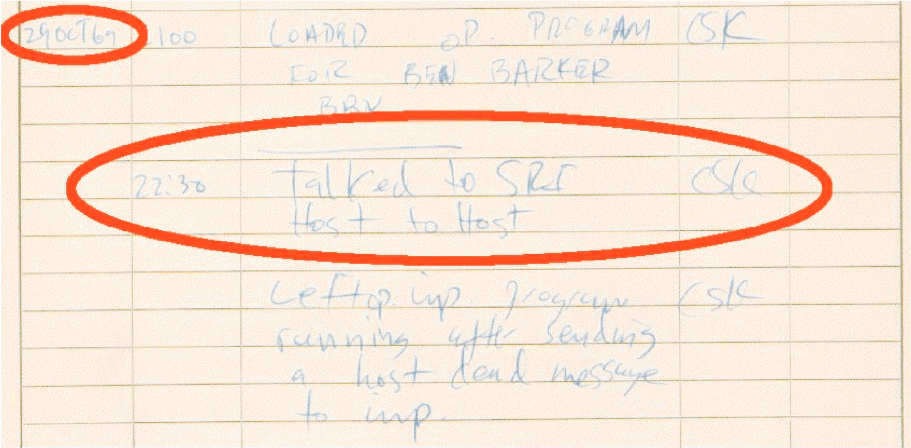
\includegraphics[width=15cm]{KLEINROCK_1ST_COM.png}
    \caption{Notes témoignant du premier message envoyé via l'ARPANET, 29 octobre 1969 (L. Kleinrock, "An Early History of the Internet"..., p.32)}
    \label{fig:enter-label}
\end{figure}

Deux ans plus tard, quinze noeuds de communication sont déjà opérationnels dans divers endroits des États-Unis. En 1972 se tient la première démonstration des capacités réticulaires de l'ARPANET; le succès est au rendez-vous, et le public apprend à connaître l'agence. La technologie évolue l'année suivante, avec le développement d'un nouveau protocole d'échange de données: c'est le \textit{Transmission Control Protocol}, qui se révèle bien plus fiable que le protocole initial NCP. Il faudra cinq autres années (1978) pour qu'un nouveau protocole, l'\textit{Internet Protocol} - IP - soit développé, afin de faire communiquer les noeuds entre eux.\\

En 1980, l'usage conjoint des deux protocoles est reconnu comme standard par le Département de la Défense américain pour ses communications\footnote{\cite[p.~34-35]{kleinrockEarlyHistoryInternet2010}}. Le TCP et l'IP se combinent définitivement en 1982, et ARPANET remplace pour de bon le NCP. C'est, encore aujourd'hui, le protocole standard d'échange de données\footnote{\cite[p.~16-17]{ceruzziAuxOriginesAmericaines2012}}. Vinton Cerf a participé au développement des deux protocoles maintenant fusionnés; cela lui vaut d'être considéré comme un des pères fondateurs d'Internet.\\

En France, malgré des conflits d'intérêts nationaux, le projet Cyclades porté par l'IRIA (Institut de Recherche en Informatique et en Automatique, future INRIA) bénéficie d'une reconnaissance certaine à l'international. Les États-Unis bénéficiant d'une longueur d'avance technologique, se connecter à leur réseau de noeuds national s'impose comme une tâche prioritaire. En conséquence, les champs de recherche de Cyclades portent notamment sur la communication entre systèmes informatiques différents. Son abandon en 1979, décidé afin de ne pas détourner des financements des projets du Minitel et de l'informatisation de la société consécutif au rapport Nora-Minc, marque le début d'une \og période glaciaire \fg{} en termes de recherche sur les réseaux à l'INRIA.\footnote{\cite[p.~41-45]{grisetMakePigFly2012}}\\

Si les ordinateurs personnels se démocratisent quelque peu dans les années 1970, leurs possibilités communicationnelles ne sont que peu exploitées... au grand dam de nombreux ingénieurs, pour qui l'échange de données en constitue précisément la principale opportunité. Ils sont avant tout utilisés pour leurs logiciels bureautiques et de loisirs, à commencer par les jeux. Les obstacles à la connexion sont d'ordre pratique: installer un logiciel spécifique, relier l'ordinateur à un modem, relier ce modem à une ligne téléphonique, avant de devoir composer un numéro local, pour seulement ensuite se connecter au service... Toutes ces démarches demandent un certain effort, d'autant qu'à l'arrivée, le prix prohibitif des communications longue distance limitait les échanges à un niveau local. Certains préfèrent se connecter la nuit, lorsque ces tarifs sont réduits.\footnote{\cite[p.~17-18]{ceruzziAuxOriginesAmericaines2012}}\\

C'est la décennie suivante qui, dans l'histoire d'Internet, est marquée par les premières initiatives commerciales. \textit{The Source}, \textit{Control Video}, \textit{Quantum Computer Services} (futur AOL), sont autant d'entreprises qui ont visé à développer un réseau performant, que ce soit pour l'échange d'e-mails ou pour la connectivité de jeux en ligne. La société \textit{Prodigy}, lancée en 1984, se distingue également par le développement d'interfaces graphiques. L'affichage devient alors plus attractif, moins austère, que le format textuel plein utilisé jusqu'alors. Cela signifie aussi l'apparition de la publicité en ligne, permettant ainsi d'amortir les coûts d'investissements et, par effet rebond, de revoir à la baisse les prix d'abonnement aux services. Ce modèle commercial est le fondement du Web d'aujourd'hui.\footnote{\cite[p.~18-19]{ceruzziAuxOriginesAmericaines2012}}\\

\section{L'invention du Web}
Jusqu'ici, nous n'avons résumé que les origines d'\textit{Internet}, et non du \textit{Web}. Les deux termes sont communément utilisés de manière interchangeable, mais ils désignent en réalité des concepts distincts.\\

En effet, Internet est avant tout une infrastructure physique composée de câbles, de satellites, de serveurs, de routeurs et d'autres équipements; la transmission de données entre des ordinateurs et autres appreils connectés partout dans le monde est définie par les fameux protocoles TCP/IP que nous avons mentionnés plus haut. Quant au Web, il s'agit d'un \og protocole de communication \fg{} (le protocole HTTP) qui va mobiliser Internet pour établir un réseau de pages, toutes liées entre elles, auxquelles nous pouvons accéder via une adresse (l'\textit{URL}, débutant par \og http://\fg{})\footnote{\cite[p.~27-28]{cardonCultureNumerique2019}}. Vint Cerf et Tim Berners-Lee, considérés respectivement comme l'inventeur d'Internet et l'inventeur du Web, s'amusent de la confusion fréquente entre les deux termes.\\
\begin{figure}[h]
    \centering
    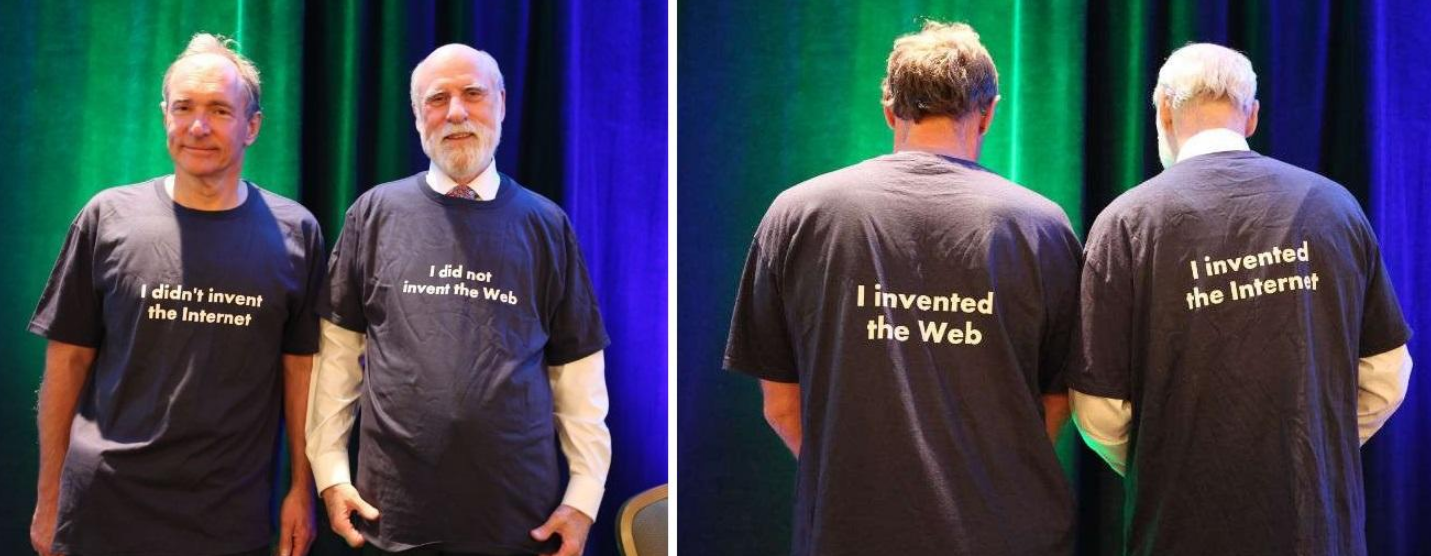
\includegraphics[width=15cm]{CERF_BERNERSLEE.png}
    \caption{Tim Berners-Lee (à gauche) et Vint Cerf (à droite). Photographie prise à l'occasion des 20 ans de la création du W3C (\textit{World Wide Web Consortium}), en 2014.}
    \label{fig:enter-label}
\end{figure}

Ce principe d'adressage par URL (\textit{Uniform Resource Locator}) et son système de liens entre pages (les liens \textit{hypertextes}) constitue le socle technique sur lequel le Web se repose. Ils permettent d'accéder à des ressources sur Internet de manière simplifiée, puisque l'on s'affranchit du besoin de connaître leurs emplacements dans un système de dossiers mis en ligne. Elles se renvoient dorénavant les unes aux autres, en formant un réseau - d'où le nom de \textit{Web} ou de \textit{Toile}. Le Web simplifie énormément l'accès à cet Internet encore restreint à un petit nombre de personnes aux compétences techniques nécessaires. Son usage s'étendra désormais bien en dehors du cadre défini par ses pionniers de l'ARPA.\footnote{\cite[p.~80-86]{cardonCultureNumerique2019}}\\

L'invention du Web, en 1989, était une réponse aux besoins d'accessibilité et de diffusion de la documentation interne du CERN (\textit{Conseil européen pour la recherche nucléaire}). Berners-Lee soumet son document intitulé \textit{Information Management: A Proposal}\footnote{Le document est présenté en annexe de son livre: \cite[p. 211-229]{berners-leeWeavingWebOriginal2000}}, dans lequel il définit la notion d'\textit{hypertexte}. Le système doit être simple et intuitif, et permettre à chacun de continuer à travailler dans son environnement de travail propre. Ainsi sont conçus les \og liens \fg, qui permettent à chacun de facilement naviguer de page en page\footnote{\cite[p.~18-20]{berners-leeWeavingWebOriginal2000}}. Le langage de balisage HTML (\textit{HyperText Markup Language}) est également créé pour écrire et structurer ces pages dorénavant enrichies de ces éléments interactifs. Pour compléter cette révolution, Berners-Lee met au point l'année suivante ce qui constituera le premier navigateur Web de l'histoire: \textit{WorldWideWeb}.\\

Le système nécessitera encore quelques adaptations techniques afin de se diffuser à l'échelle globale, notamment en développant des versions utilisables par les utilisateurs de PC, Macintosh et d'Unix (le système NeXT, utilisé par le CERN, étant propre à celui-ci)\footnote{\cite[p.~55-56]{berners-leeWeavingWebOriginal2000}}. La technologie se consolide et se renforce. Mais il faut attendre le 30 avril 1993 pour que le signal de départ du Web public soit tiré. Ce jour-là, le CERN annonce renoncer à ses droits d'auteur sur les technologies du Web - qui passent donc dans le domaine public - et publie le code permettant à quiconque de produire du contenu HTML.\footnote{\cite[p.~87-88]{cardonCultureNumerique2019}}\\ 

D'autres navigateurs ne tardent pas à être développés, dont \textit{Mosaic}, le premier navigateur public. Il est développé par l'équipe du \textit{National Center for Supercomputing Applications} (NCSA) de l'Université de l'Illinois, dirigée par Marc Andreessen. \textit{Mosaic} innove en permettant que les images soient directement intégrées dans les pages Web, les rendant ainsi visuellement bien plus attrayantes. Le même Andreessen fonde ensuite \textit{Netscape} en 1995, année qui verra également le développement d'\textit{Internet Explorer} et d'\textit{AltaVista}. Parallèlement, la quantité de contenu mis en ligne explose: le nombre de sites Web passe de 130 en juin 1993, à plus de 230.000 en 1996.\footnote{\cite[p.~86-88]{cardonCultureNumerique2019}}\\

Cette première phase d'expansion perdurera jusqu'au début des années 2000. Elle est communément désignée sous les termes de \textit{Web 1.0} ou de \textit{Web des documents}. Elle était marquée par la nature statique des pages Web. Les sites sont alors principalement conçus comme des collections de pages HTML, dont les seules interactions possibles prenaient la forme de liens hypertextes.\\

En termes de contenu, les sites du \textit{Web 1.0} sont souvent centrés sur la présentation d'informations de base: descriptions de produits, coordonnées d'entreprise, documents en ligne. Ils sont avant tout des vitrines, mettant en avant des informations statiques pour un public en quête d'informations. Les médias se mettent à proposer des versions numérisées de leurs contenus imprimés. Quant aux interactions sociales, elles étaient limitées principalement aux forums de discussion et aux chats en ligne, tout en restant restreintes par rapport à la connectivité omniprésente d'aujourd'hui.\footnote{Le développement de celles-ci fait partie intégrante de ce que l'on définit comme le \textit{Web 2.0}, que nous ne détaillerons pas dans ces pages}\\


\section{Les technologies sémantiques}

L'une des principales limitations du Web pré-sémantique résidait dans l'absence de structure et de contextualisation les données. Chaque page était conçue de manière indépendante, en format plein texte. Les informations présentées étaient largement conçues pour être lues et comprises par les humains, et eux seuls. La machine, elle, est incapable d'analyser un document en ligne, que ce soit du point de vue de son type, de sa structure, ou des termes et concepts qu'il contient. \og Autrement dit, le \textit{Web 1.0} fait ses traitements à l'aveugle, en ne prenant en compte que le format de codage des contenus, mais non la sémantique de ces derniers \fg\footnote{\cite[p.~24-25]{bachimontSensWebSemantique2011}}.\\

Certes, des recherches par mots-clefs sont possibles, par balayage d'une page à la recherche d'une suite de caractères; cependant, elles montrent leurs limites dès qu'il s'agit de gérer le genre et le nombre d'un terme, de désambiguïser deux termes polysémiques, ou, au contraire, de renvoyer des termes synonymes ou relevant du même champ lexical. De plus, la pratique consistant à glisser des mots-clefs cachés au sein des pages, afin d'augmenter son référencement, donne de nombreux faux positifs. Mobiliser les ressources de la machine devient nécessaire pour assister l'homme dans sa quête d'information.\\


Ce sont ces constats qui ont conduit Tim Berners-Lee à définir la notion de \textit{Web sémantique}, dans deux textes fondateurs de 1998 et 2001\footnote{Voir: \cite{berners-leeSemanticWebRoad1998} et \cite{berners-leeSemanticWeb2001}}. Un nouveau formalisme des données, accessible à des non-spécialistes, doit pouvoir permettre au  Web de traiter des données hétéroclites et les (ré)ordonner entre elles. \og Le Web sémantique n'est pas un Web à part, mais une extension du Web actuel, dans lequel l'information est dotée d'une signification bien définie, ce qui permet aux ordinateurs et aux personnes de mieux travailler en coopération \fg\footnote{\og The Semantic Web is not a separate Web but an extension of the current one, in which information is given well-defined meaning, better enabling computers and people to work in cooperation. \fg. \cite{berners-leeSemanticWeb2001}}.\\ 

Il est là question d'un nouveau modèle. Tout comme la naissance du Web était caractérisée par la mise à disposition de documents à travers un adressage hypertexte, les technologies sémantiques ont pour objectif de mettre en lumière l'information au sein des documents du Web. Ceux-ci sont alors découpés en une série d'éléments dont le contenu est balisé par un marquage signifiant: ces sont les \textit{microdonnées}\footnote{\cite[p.~82]{mesguichBibliothequesWebEst2017}}. Celles-ci permettent, par exemple, d'identifier qu'une page Web concerne un livre, et d'opérer une distinction entre les informations relatives à son titre, à son auteur, son genre, son résumé, les oeuvres similaires, etc.\\

Les moteurs de recherche sémantiques se développent dans les années 2000. Ils traitent ces microdonnées et déchiffrent ainsi le contenu d'une page Web, améliorant ainsi la pertinence des résultats d'une requête. Les termes sont compris dans un sens plus vastes à travers la définition de schémas de connaissances, qui permettent de déduire le contexte d'une requête, ses résultats connexes, de gérer les questions de synonymies, de genre, de nombre, etc.\\

Des fonctionnalités se développent également pour mettre en valeur ces schémas de connaissances. Depuis 2012, Google - qui, avec plus de  90\% des recherches effectuées, est le moteur le plus utilisé au monde\footnote{91,47\% en France entre juillet 2022 et juillet 2023, et 92,08\% à l'échelle mondiale, selon les données compilées par le site \textit{Statcounter}. \url{https://gs.statcounter.com/search-engine-market-share (visité le 10/08/2023)}} - met ainsi à contribution son \textit{Google Knowledge Graph} (la notion de graphe de connaissance sera développée plus loin dans ces pages) pour proposer des encadrés récapitulatifs facilitant l'accès à de l'information connexe. \\
\begin{figure}[h]
    \centering
    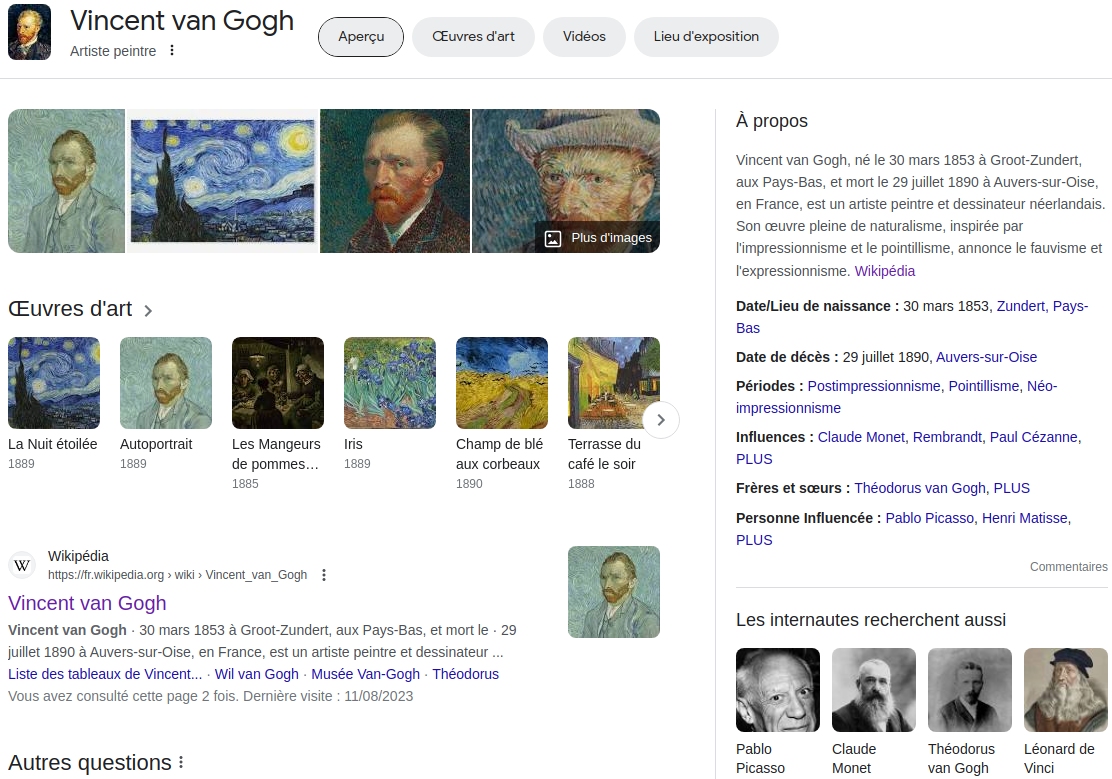
\includegraphics[width=16cm]{VANGOGH_GOOGLE.png}
    \caption{Une vision familière: capture d'écran du 11 août 2023, montrant l'encadré issu du \textit{Google Knowledge Graph}, résultant d'une recherche de \og Vincent van Gogh \fg{} sur Google.}
    \label{fig:GKG_Van_Gogh_11aout2023}
\end{figure}

Les performances des moteurs de recherche ont néanmoins pu susciter des espoirs démesurés envers cette technologie. Le terme de \textit{Web sémantique} n'y est probablement pas étranger. Or, l'absence de consensus terminologique peut être révélateur de conceptions différentes\footnote{\cite[p.~22]{amarBienvenueDansGigantesque2011}}. Déjà en 2003, Michael Uschold en relevait les contradictions dans un article au titre évocateur\footnote{\cite[p.~26]{uscholdWhereAreSemantics2003}}. Tim Berners-Lee a lui-même reconnu l'ambiguïté du terme, car \og la sémantique [s'intéressant] au sens du langage pour en déduire des constructions logiques [...], certains ont pensé qu'il s'agissait d'un Web qui permettrait par exemple d'effectuer des recherches sur Internet en posant des questions sous forme de phrases, en langage naturel. Or ce n'est pas son but \fg\footnote{\cite{berners-leeWebChangeDimension2019}}. En effet, cela se rapporte davantage à ce que l'on a coutume d'appeler l'Intelligence Artificielle - qui consiste à \og entraîner les machines à se comporter comme des personnes \fg\footnote{\cite{berners-leeSemanticWebRoad1998}}.\\


\section{Vers le Web de données}
\subsection{Un simple glissement lexical?}
Les institutions scientifiques participent à l'effervescence initiale autour des technologies sémantiques. Elles développent leurs propres modèles de connaissances, dont la complexité est à la hauteur de leurs besoins. Elles négligent cependant la publication de leurs données sur le Web, en les stockant \og quelque part, enterrées dans une archive Zip \fg{} \footnote{\og buried in a zip archive somewhere\fg. \cite{berners-leeLinkedData2006}}. Quant au secteur industriel, il ne s'est que peu impliqué dans la démarche\footnote{Voir \cite[p.~37-38]{bermesWebSemantiqueBibliotheque2013} et \cite{poupeauBilan15Ans2016}}.\\

Cela contraint Berners-Lee à pporter des précisions sur sa vision du Web sémantique en 2006, en introduisant le concept de \textit{Linked Data} dans une note du même nom:
\begin{quotation}
    \og Le web sémantique ne consiste pas seulement à mettre des données sur le web. Il s'agit de créer des liens, afin qu'une personne ou une machine puisse explorer le web de données. Avec les données liées, lorsque vous en possédez certaines, vous pouvez trouver d'autres données connexes. Comme le web de l'hypertexte, le web de données est construit à partir de documents sur le web. Toutefois, contrairement au web de l'hypertexte, où les liens sont des ancres de relations dans des documents hypertextes écrits en HTML, pour les données, il s'agit de liens entre des éléments arbitraires décrits par RDF\fg\footnote{\og The Semantic Web isn't just about putting data on the web. It is about making links, so that a person or machine can explore the web of data. With linked data, when you have some of it, you can find other, related, data. Like the web of hypertext, the web of data is constructed with documents on the web. However, unlike the web of hypertext, where links are relationships anchors in hypertext documents written in HTML, for data they links between arbitrary things described by RDF\fg. \cite{berners-leeLinkedData2006}}
\end{quotation}

La référence à un \og Web de données \fg{} plutôt qu'à un \og Web sémantique \fg{} n'est pas neuve. La première feuille de route de 1998 mettait déjà les deux notions sur un pied d'égalité\footnote{\og Ce document est un plan visant à réaliser un ensemble d'applications connectées pour les données sur le Web, de manière à former un web de données (web sémantique) logique et cohérent\fg{} (\og This document is a plan for achieving a set of connected applications for data on the Web in such a way as to form a consistent logical web of data (semantic web)\fg). \cite{berners-leeSemanticWebRoad1998}}. Rétrospectivement, Berners-Lee considère que le \textit{Web sémantique} aurait dû être appelé \textit{Web de données} dès le départ - bien qu'il soit aujourd'hui \og trop tard pour changer de nom \fg\footnote{\cite{berners-leeWebChangeDimension2019}}.\\

Dans \textit{Linked Data}, Berners-Lee pose les quatre principes fondateurs du \textit{Web de données}: l'usage des URI comme identifiants de ressources, l'usage du protocole HTTP pour les formuler, l'utilisation de formats spécifiques et de SPARQL, et l'agencement des URI entre eux selon des liens sémantiques. Le \textit{Web de données} se présente donc avant tout comme la définition d'un nouveau réseau: non plus de document en document (comme c'était le cas pour le \textit{Web 1.0}), mais bien entre données, les \textit{Linked Data}. \og Créer un lien automatique pour relier les données qui sont stockées dans les différents fichiers et bases de données de nos ordinateurs \fg\footnote{\cite{berners-leeWebChangeDimension2019}}, et s'affranchir ainsi du cloisonnement que constituent les activités propres à chaque institution.\\

En d'autres termes, il s'agit de déployer une infrastructure pour placer la donnée au centre de la démarche, et non plus le processus dans lequel elle est produite. La voie vers le réemploi et l'interopérabilité est pavée. Si le concept semble avoir été quelque peu \og rétréci \fg{} par rapport aux espoirs que certains ont pu mettre aux premières heures du \textit{Web sémantique}, il en devient plus compréhensible, et donc plus facilement assimilable\footnote{\cite[p.~23]{amarBienvenueDansGigantesque2011}}.\\

\subsection{La notion de donnée}

La définition affinée place maintenant la donnée au centre du processus. Mais dans ce cas, qu'est ce qu'une donnée?\\

Là encore, nous pouvons nous heurter à un problème de définition, car \og le concept de donnée mériterait à lui seul un ouvrage entier \fg{} et a, la plupart du temps, été défini uniquement par l'exemple\footnote{\cite[p.~41]{borgmanQuEstceQue2020}}. Pour ne pas surcharger ces pages, nous procéderons de même, en reprenant les distinctions que fait Serge Abiteboul entre la \textit{donnée}, l'\textit{information} et la \textit{connaissance}\footnote{\cite{abiteboulSciencesDonneesLogique2012}}: 
\begin{quotation}
    \og Des mesures de température relevées chaque jour dans une station météo, ce sont des données. Une courbe donnant l’évolution dans le temps de la température moyenne dans un lieu, c’est une information. Le fait que la température sur Terre augmente en fonction de l’activité humaine, c’est une connaissance.
    [...]
    \begin{itemize}
        \item Une donnée est une description élémentaire, typiquement numérique pour nous, d’une réalité. C’est par exemple une observation ou une mesure.        
        \item À partir de données collectées, de l’information est obtenue en organisant ces données, en les structurant pour en dégager du sens.        
        \item En comprenant le sens de l’information, nous aboutissons à des connaissances, c’est-à-dire à des « faits » considérés comme vrais dans l’univers d’un locuteur, et à des « lois » (des règles logiques) de cet univers.\fg{}
    \end{itemize}
\end{quotation}

Le \textit{Web de données} à donc vocation à structurer le savoir humain selon ses plus petites mais néanmoins indispensables briques. 

\subsection{Les \textit{Linked Open Data}}
Créer du lien entre données nécessite cependant que les données soient partagées, et rendues consultables sur le Web. En ceci, les objectifs du Web de données rejoignent des préoccupations citoyennes plus larges, telles que l'\textit{Open Data} - qui revendique la mise à disposition des données produites par les institutions publiques (et dont Barack Obama fit un argument pour sa campagne électorale de 2009)\footnote{\cite[p.~57]{bermesWebSemantiqueBibliotheque2013}}.\\

En 2010, Berners-Lee met à jour sa note initiale. Il se positionne en faveur de données liées ET ouvertes, libres d'accès, réutilisables: ce sont les \textit{Linked Open Data}. Dans le but d'à la fois en préciser la portée et de créer de l'effervescence autour de lui, Berners-Lee en définit une échelle de qualité. La notation est comprise entre une et cinq étoiles. 
\begin{itemize}
    \item 1 étoile: Les données sont rendues disponibles sur le Web, peu importe le format tant que leur réemploi est autorisé (ce qui leur permet d'être catégorisées comme \textit{Open data});
    \item 2 étoiles: Les données sont rendues disponibles dans un format structuré (tel qu'un tableur Excel), soit un format lisible par une machine;
    \item 3 étoiles: Les données sont rendues disponibles dans un format structuré et non-propriétaire (c'est-à-dire dont les spécifications techniques ne sont pas contrôlées par des intérêts privés), tel que CSV à la place d'Excel;
    \item 4 étoiles: Les données sont rendues disponibles dans un format structuré et non-propriétaire, et utilisent les standards du W3C (RDF et SPARQL) pour identifier les données;
    \item 5 étoiles: Les données sont rendues disponibles dans un format structuré et non-propriétaire, utilisent les standards du W3C susmentionnés et lient leurs données à des données extérieures pour fournir du contexte.
\end{itemize}

\begin{figure}[h]
    \centering
    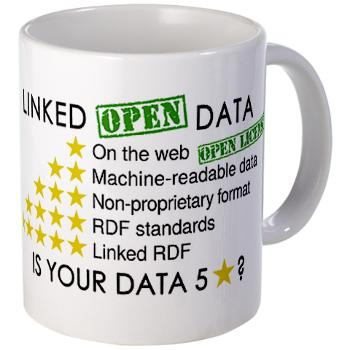
\includegraphics[width=10cm]{LINKED_OPEN_DATA.jpg}
    \caption{L'échelle de qualité des données liées ouvertes, telle que définie par Tim Berners-Lee en 2010.}
    \label{fig:enter-label}
\end{figure}


\subsection{L'émergence d'un réseau de données}
Dès lors, de nombreuses initiatives vont émerger pour décloisonner et interconnecter différents jeux de données. Les jeux de données sont mis en forme selon les principes du RDF pour mettre en oeuvre une nouvelle forme d'interopérabilité, basée sur le lien.\\

La première application d'envergure des principes du Web de données est l'initialisation du \textit{Linked Open Data Cloud} par DBPedia\footnote{Mis au point par l'université de Leipzig, l'université libre de Berlin et la société Openlink, DBPedia a pour activité de générer des données ouvertes et liées en analysant le contenu des pages Wikipedia.}. Il compte aujourd'hui 1255 jeux de données connectés par 16174 liens\footnote{Selon le site du \textit{Cloud}: \url{https://www.lod-cloud.net/\#about} (visité le 22/08/2023).}. Il s'agit d'un réseau collaboratif: dès qu'un jeu de données obéit aux règles du Web de données et atteint une taille et une interconnexion minimales, il peut être proposé à DBPedia pour être inséré dans le réseau.\\

Parmis les données liées via le \textit{Linked Open Data Cloud}, nous pouvons citer Wikidata, Geonames, VIAF, ISNI, la BnF... La liste est longue, mais nous retiendrons que ces jeux de données sont classés selon sept types: les ressources d'intérêt général, les ressources sociales, les ressources géographiques, les données gouvernementales, les ressources multimédias, les ressources biologiques et médicales, et enfin les ressources bibliographiques.\\

Le milieu bibliothéconomique s'empare également de la technologie. Entre mai 2010 et août 2011, la mission du \textit{Groupe d’incubation du W3C \og Bibliothèques et web de données \fg{}} explore les prérequis et les avantages d'une application en bibliothèque. Le rapport final\footnote{\cite{bakerRapportFinalGroupe2012}.} recommande notamment l'identification des jeux de données à exposer, le renforcement de la participation du secteur dans le Web sémantique, la mise en place des URI, ainsi que la définition de modélisations en RDF. La BnF ouvre ses entrepôts de données au public peu de temps après, à travers son nouveau portail \textit{Data BNF}\footnote{\url{https://www.bnf.fr/fr/databnffr} (visité le 22/08/2023).}; son déploiement entraîne, en quelques années, une multiplication par six du nombre de visites journalières sur le site principal\footnote{\cite[p.~59]{illienWebSemantiqueNouveau2015}.}.\\

Depuis 2015, les Archives Nationales de France, en collaboration avec un groupe d'experts sur la description archivistique (EGAD) du Conseil International des Archives (CIA), se sont engagées dans un projet pilote visant à démontrer l'applicabilité des technologies sémantiques à la mise en valeur des données archivistiques. Celles-ci incluent bien sûr des descriptions de fonds, mais également de producteurs, d'entités géographiques et politiques (présentes et passées). Le projet \textit{Records in Contexts} est appelé à remplacer les standards existants en archivistique.\\




\chapter{Les principes du Web de données}

Le Web de données repose sur un stockage dans une base de connaissances ouvertes au réemploi, depuis laquelle des entités seront extraites pour être éditorialisées. Ces bases sont modélisées en graphe de connaissances, suivent le modèle RDF, et disposent de leur propre langage de requête: SPARQL. Les pages suivantes passeront en revue chacune de ces ces caractéristiques. 


\section{Le graphe de connaissance}
De manière générale, la modélisation des données est une étape essentielle dans le processus de gestion de l'information. Cette pratique crée un fil conducteur guidant la manière dont les données sont saisies, stockées et consultées. Cela facilite leur compréhension et leur analyse, mais également leur pérennité et leur évolutivité.\\

Dans le cas des technologies sémantiques, la modélisation prend la forme du graphe de connaissance, qui consiste à structurer l'information par la définition de relations entre entités - des personnes, lieux, documents, concepts, etc. Celles-ci vont être représentées par des \og noeuds \fg, connectés par des \og arêtes \fg{} qui représentent ces liens.\\

En soi, un graphe est une représentation partielle des connaissances. Une petite base de données d'artistes pourrait par exemple être modélisée de cette manière:
\newpage
\begin{figure}[h]
    \centering
    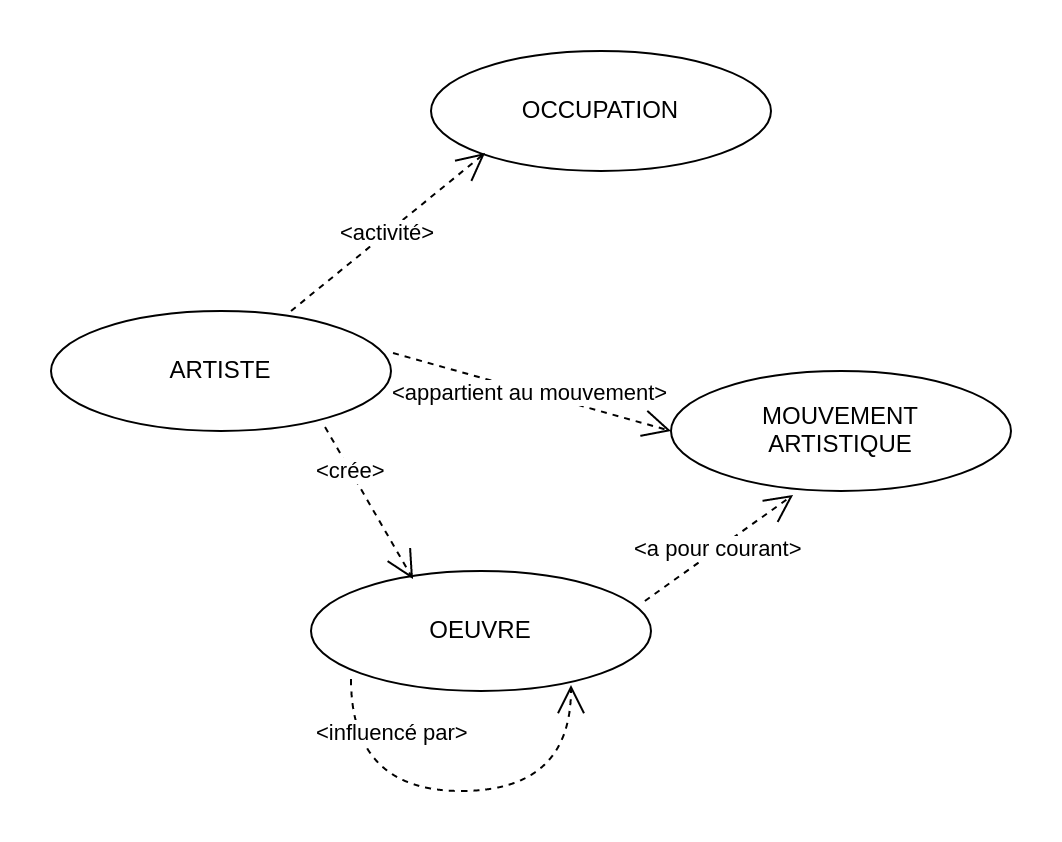
\includegraphics[width=12cm]{ARTISTES_MEM_GRAPH.png}
    \caption{Exemple d'une modélisation en graphe.}
    \label{fig:enter-label}
\end{figure}

L'usage des relations permettant d'articuler des entités, ce type de graphe de connaissance peut catégorisé comme \og orienté Entités \fg. Il constitue le modèle le plus fréquent, bien qu'il ne soit pas sans défaut. Il existe aussi des graphes de connaissances \og orientés Évènement \fg\footnote{\cite{poupeauQuelEvenementOu2010}}, \hyperref[mod-evenement]{que nous aurons l'occasion de présenter ultérieurement}.\\

Notons que ce ne sont pas les seuls modèles de graphes existants. Le \textit{Property Graph} est ainsi utilisé par nombre de poids lourds mondiaux de l'informatique et de l'électronique\footnote{\cite{poupeauAudelaLimitesQue2018}}. Cependant, il suit son propre modèle (Apache Tinkerpop au lieu de RDF) et son langage de requêtes (Gremlin plutôt que SPARQL). Il ne fait donc pas partie du champ du Web de données.\\

Bien sûr, les modélisations en graphe utilisées par les institutions sont plus complexes, et sont adaptées à la nature de leurs activités et de leurs besoins. Nous avons reproduit, \hyperref[annexe-modconcept]{en Annexes}, les modélisations en graphes d'\textit{IFLA-LRM} (utilisé par les bibliothèques dans le cadre de la \og Transition Bibliographique\fg), de \textit{RiC-CM} (destiné au déploiement prochain de \textit{Records in Contexts}), ainsi que de celui que nous avons produit dans le cadre de notre stage à l'AAFS.\\




\section{Le RDF}
Le RDF (\textit{Resource Description Framework}) a été développé par le World Wide Web Consortium (W3C) pour répondre aux besoins croissants de gestion et de représentation des données sur le Web. Il peut être considéré comme une façon de représenter des données préalablement modélisées sous forme de graphe. Il permet de donner une signification à un lien standardisé entre deux ressources. Ce lien est le vecteur d'interopérabilité entre jeux de données.\\


\subsection{Principes du RDF}
La modélisation en graphe que nous avons produite ci-dessus est une représentation conceptuelle, destinée à être comprise par des humains. Bien qu'il existe des outils pour visualiser les données sous cette forme, ce n'est pas la façon dont elles sont exprimées. Le principe fondateur du le RDF consiste à \og découper \fg{} un graphe en une série d'assertions basiques, de la même manière qu'une phrase simple est composée d'un verbe, d'un sujet et d'un complément. Ces phrases sont appelées des triplets.\\

Chacun d'eux est composé de trois éléments: le sujet, le prédicat et l'objet.
\begin{itemize}
    \item Le sujet représente l'entité principale dont des informations sont fournies;
    \item Le prédicat indique la nature de la relation entre un sujet et un objet;
    \item L'objet représente la valeur ou l'entité liée au sujet par le prédicat.
\end{itemize}

Si nous reprenons notre modélisation d'exemple, et que nous remplaçons les grandes catégories par des entités potentielles, nous pourrions obtenir ceci: 
\newpage
\begin{figure}[h]
    \centering
    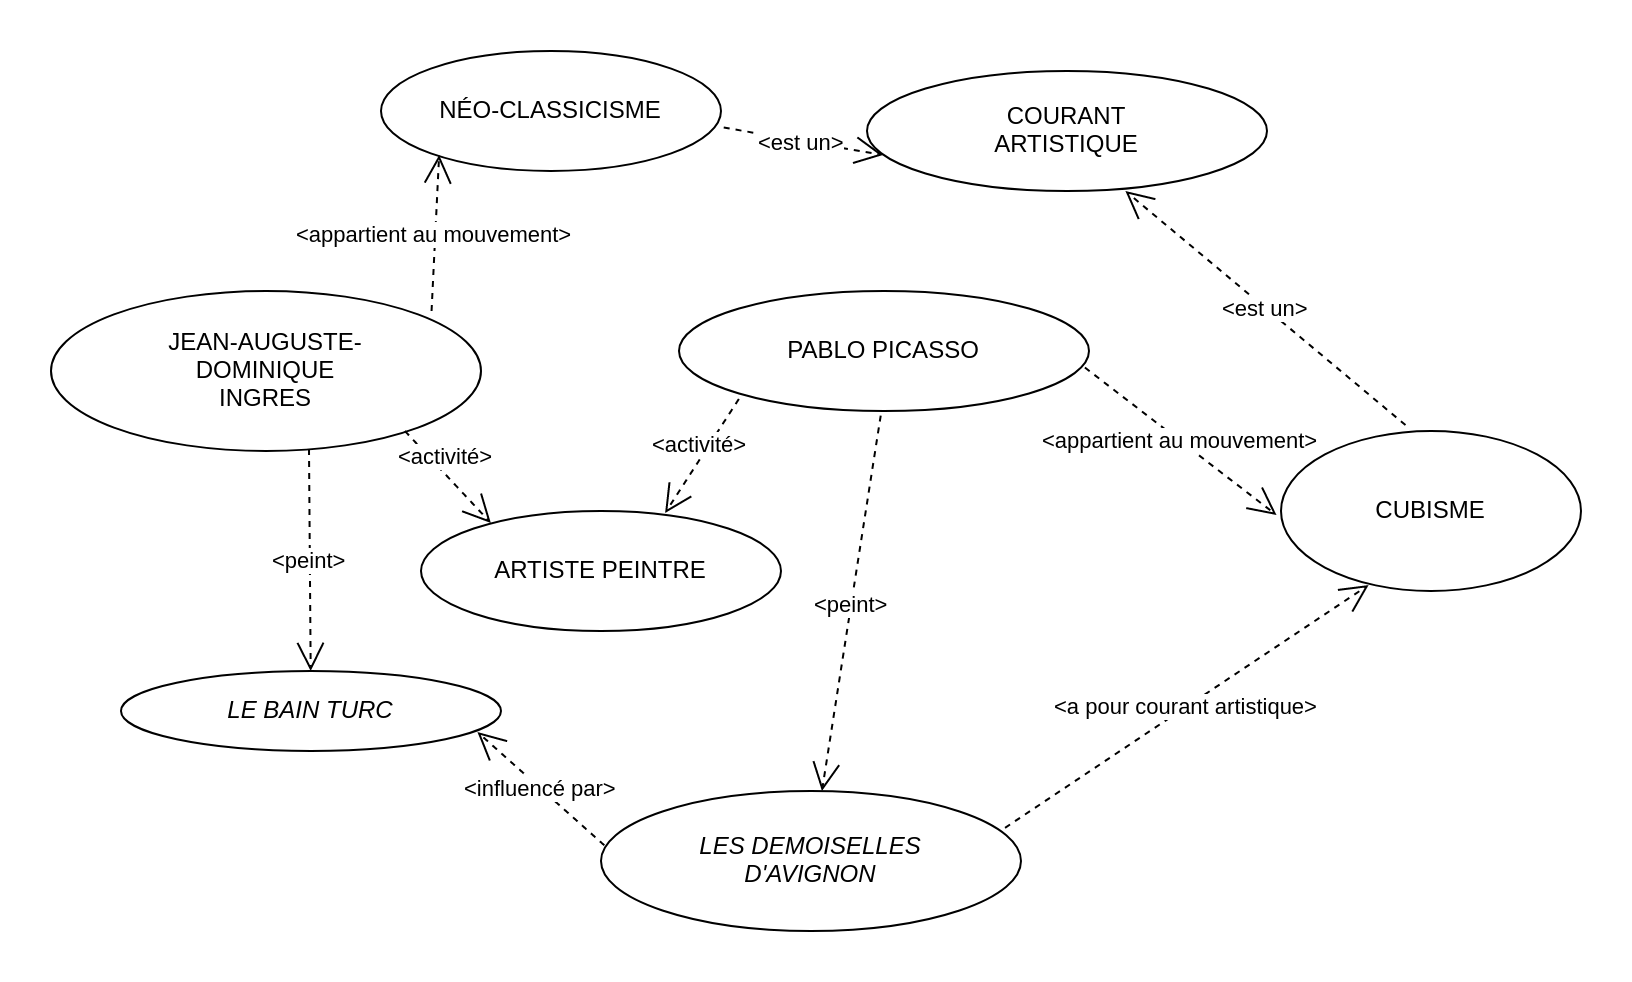
\includegraphics[width=17cm]{ILLU_MEMOIRE_GRAPHE.png}
    \caption{Notre exemple précédent, rendu plus concret.}
    \label{fig:enter-label}
\end{figure}

Si, à présent, nous lui appliquons le principe des triplets, ce graphe peut être décomposé en la série d'assertions suivante:
\begin{center}    
\begin{tabular}{|c|c|c|}
\hline
sujet & prédicat & objet \\
\hline
Pablo Picasso & a pour activité & artiste peintre \\
Jean-Auguste-Dominique Ingres  & a pour activité & artiste peintre \\
Jean-Auguste-Dominique Ingres & peint & \textit{Le Bain Turc} \\
Pablo Picasso & peint & \textit{Les Demoiselles d'Avignon}\\
\textit{Les Demoiselles d'Avignon} & est influencé par & \textit{Le Bain Turc}\\
\textit{Les Demoiselles d'Avignon} & a pour courant artistique & Cubisme \\
Pablo Picasso & appartient au mouvement & Cubisme \\
Cubisme & est un & Mouvement artistique \\
Néo-classicisme & est un & Mouvement artistique \\
Jean-Auguste-Dominique Ingres & appartient au mouvement & Néo-Classicisme \\
\hline
\end{tabular}\
\end{center}


Chaque entité peut tantôt être un sujet, tantôt un objet. La multiplication de ces triplets va construire tout un réseau d'entités reliées entre elles. Le graphe traite également chaque élément comme une entité distincte, indépendamment du fait qu'il s'agisse d'un objet physique (comme \textit{Les Demoiselles d'Avignon} et \textit{Le Bain Turc} de notre exemple), d'une personne (Picasso, Ingres) ou d'un concept (Cubisme, Néo-Classicisme). En effet, le système de RDF est profondément décentralisé: chaque entité occupe une place dans le réseau, sans notion de préséance ou de hiérarchie.\\

La structuration des données par assertions successives supporte particulièrement bien les changements et ajouts, comparé à d'autres structures de bases de données dont la portée est locale:
\begin{itemize}
    \item Ajouter un type d'information nouveau dans une base de données relationnelle impose de comprendre la structure des tables, éventuellement de la revoir, et de s'assurer que les modifications ne créent pas de conflits ou de redondances avec les autres tables.\footnote{\cite[p.~53-54]{vanhoolandIntroductionAuxHumanites2016}} 
    \item Une modification de la structure en XML des fichiers d'une base de données de documents peut être délicate. Si l'ajout d'un élément optionnel ne pose pas de problème majeur, la modification du nom d'une balise ou la transposition d'un attribut en une balise peut créer de la nouveauté ou des incohérences que le parseur (qui parcourt le document) aura du mal à interpréter sans modifications.\footnote{\cite[p.~63-64]{vanhoolandIntroductionAuxHumanites2016}}
    \item En revanche, une base de données en RDF est complètement décentralisée et n'est, en somme, qu'une succession de triplets. Les modifications se font simplement en ajoutant/supprimant/modifiant autant de triplets que nécessaire\footnote{\cite[p.~72]{vanhoolandIntroductionAuxHumanites2016}}. Dans notre exemple, ajouter une oeuvre à un artiste ou ajouter des dates pour définir l'âge d'or du Néo-classicisme ne change en rien la validité ou la lecture des autres triplets. 
\end{itemize}


\subsection{Typologie des sujets et des objets}
\subsubsection{Les URI}

Comme stipulé dans la note de Tim Berners-Lee, le RDF va devoir articuler des ressources entre elles. Celles-ci doivent être uniques, identifiées, et désambiguïsées. Dans ce but, le RDF place les URI (\textit{Uniform Resource Identifier}) au coeur de son modèle: leur emploi pour identifier une ressource constitue le premier principe fondateur dicté par Berners-Lee: sans cela, \og on ne peut parler de Web sémantique \fg{} \footnote{\og If it doesn't use the universal URI set of symbols, we don't call it Semantic Web\fg. \cite{berners-leeLinkedData2006}}.\\

Un URI est un lien renvoyant vers une page Web. Il est similaire à un URL classique, mais se double d'une exigence de pérennité - indispensable, dans la mesure où l'architecture du Web de données repose sur eux. La pérennité est assurée par l'institution qui exprime ses entités sous cette forme.\\

L'unicité d'un URI est également essentielle. Si une institution possède déjà un plan de nommage interne pour désambiguïser les ressources qu'elle manipule au quotidien, alors la transformation de ses identifiants locaux en URI sera simplifiée. Il peut suffire d'ajouter un identifiant de l'institution devant l'identifiant de sa ressource. Cet identifiant institutionnel peut être attribué par un organisme tiers, ou bien être constitué par un code la représentant au sein d'un annuaire commun à plusieurs institutions. \footnote{\cite{ministeredelacultureetdelacommunicationIdentifiantsPerennesPour2014}}\\

\large
$$
\underbrace{\underbrace{http://}_{scheme}\underbrace{ark.bnf.fr/}_{autorit\acute{e}}}_{adressage}\underbrace{\underbrace{ark:}_{ID}\underbrace{/12148}_{entit\acute{e}}\underbrace{/cb12462063r}_{identifiant}}_{identifiant ARK}
$$
\normalsize
Cet URI provient de la BnF, et utilise le format d'identifiant ARK. Nous voyons que l'identifiant ARK n'est qu'une partie de l'URI. L'adressage renvoie vers le service qui va traiter l'identifiant ARK, et afficher une page en conséquence. Par défaut, la BnF va réadresser cet URI vers son Catalogue Général; cependant, un autre adressage permettrait d'afficher la même ressource sur un portail différent. Un résolveur interne permet la redirection vers l'un ou l'autre service.\footnote{\cite{ministeredelacultureetdelacommunicationIdentifiantsPerennesPour2014}}\\

Notons que le schème doit obligatoirement avoir recours au protocole HTTP (ou HTTPS). Il s'agit du deuxième principe fondateur de Tim Berners-Lee pour un Web de données.\footnote{\cite{berners-leeLinkedData2006}}\\

L'indentifiant ARK est consituté de plusieurs parties. 
\begin{itemize}
    \item La première est le type d'identifiant, soit ARK dans ce cas-ci (bien qu'il en existe d'autres);
    \item La seconde est le Numéro d'Entité Nommante (\textit{NAAN}, pour \textit{Name Assigning Authority Number}), attribué par la \textit{California Digital Library} (qui maintient le système ARK). Ainsi, 12148 sera un numéro commun à tous les URI émis selon le format ARK par la BnF, tandis que 67717 concernera ceux émis par le Ministère de la Culture;
    \item La troisième, l'identifiant proprement dit, est attribué de manière opaque par la BnF à cette ressource, avec des garanties d'unicité et de pérennité.\footnote{\cite{bibliothequenationaledefranceIdentifiantARKArchival2018}}.
\end{itemize}\\


\subsubsection{Les noeuds blancs}

En RDF, il arrive qu'aucun URI n'existe pour désigner une ressource que l'on veut pourtant documenter. Dès lors, une base de données en RDF peut recourir aux \textit{noeuds blancs}. Ils n'ont pas d'identifiant global unique et stable, et ne sont identifiés qu'à l'intérieur d'un graphe RDF précis. Ce sont des noeuds locaux\footnote{\cite[p.~76-78]{bermesWebSemantiqueBibliotheque2013}.}. Nous sortons alors du \textit{Web de données} tel que défini par Tim Berners-Lee.\\

Ils sont communément intégrés dans les triplets selon la syntaxe \og \_: \fg{} (\textit{underscore} et \textit{deux-points} suivi d'un numéro d'identification)\footnote{\cite[p.~13]{maillotApercusRechercheInterroger2014}}.\\


Malgré qu'ils ne soient pas identifiés par des URI, ces noeuds ont bel et bien une place dans le graphe. Aussi, des affirmations à leur sujet (tels qu'un titre, un numéro de référence, une description...) sont tout à fait valables et leur permettent de leur donner une existence, tant dans une base de données en RDF que pour une éditorialisation sur le Web. Il ne seront cepandant jamais utilisés comme URI par d'autres institutions. 

\subsubsection{Données textuelles}

Les URI constituent un des piliers de la réutilisation des données. Cependant, leur emploi en tant qu'objet n'est pas automatique. En effet, une entité ne peut se décrire uniquement à travers des relations avec d'autres entités. Ainsi, le résumé ou le titre d'un ouvrage, le numéro d'inventaire d'une oeuvre, la description physique d'un document, sont autant de cas où le type de donnée textuel sera adopté.\\

Techniquement, rien n'empêche cependant de renseigner une valeur textuelle là où un URI aurait été possible ou souhaitable. Data BnF a notamment recours à cette option, car toutes les données de ressources du Catalogue Général n'ont pas été reversées sur ce portail. La création d'URI pour une ressource n'est en effet pas automatique, si la connectivité ou le réemploi de celle-ci est estimé trop limité\footnote{\cite[p.~3]{ministeredelacultureetdelacommunicationIdentifiantsPerennesPour2014}.}.\\ 
\begin{figure}[h]
    \centering
    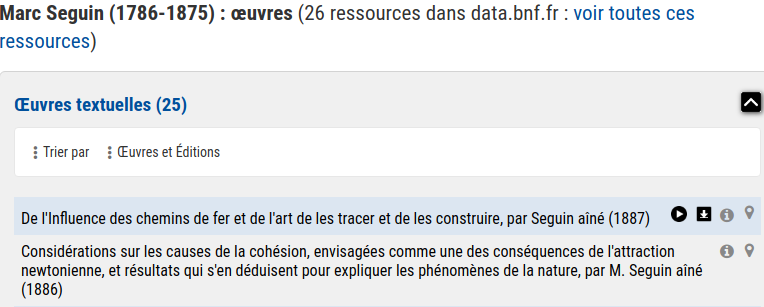
\includegraphics[width=17cm]{SEGUIN_DATABNF_TXT.png}
    \caption{Les deux premiers ouvrages de Marc Seguin sont entrés sous format texte dans Data BnF (capture d'écran du 26 août 2023)}
    \label{fig:enter-label}
\end{figure}\\
Cela pose cependant deux problèmes\footnote{\cite[p.~76]{bermesWebSemantiqueBibliotheque2013}}. Premièrement, cela matérialise des questions d’ambiguïtés, puisqu'un traitement automatique d'une chaîne de caractère ne pourra faire la différence entre plusieurs objets ayant le même nom (l'homonymie), ou un seul objet ayant plusieurs noms (synonymie). Deuxièmement et conséquemment, cet objet ne constitue dès lors plus une entité que nous pouvons réemployer pour émettre de nouvelles assertions à son sujet.\\


Malheureusement, renseigner une donnée sous forme textuelle n'est pas toujours un choix. Ainsi, cette problématique a été mise en lumière lors du traitement des données de bibliothèque de l'AAFS: de part leurs restitutions trop sommaires dans le fichier d'inventaire, nombre de noms d'auteurs n'ont pu être alignés sur les notices d'autorité de la BnF par des procédés automatisés. 616 URI d'auteurs ont pu être récupérés et insérés dans Omeka-S, et 1684 sont entrés sous forme textuelle; le reste devra se poursuivre manuellement. Une fois les URI d'auteurs récupérés, un nouvel alignement automatisé permettra de récupérer les URI des ouvrages référencés dans le Catalogue Général et/ou sur Gallica. Ce cas illustre que le recours au format textuel peut également constituer une solution temporaire, le temps d'améliorer la qualité des données. 


\subsubsection{Le cas des dates}
Les informations de dates sont essentielles à la découvrabilité d'une ressource. Pour cette raison, des dates entrées sous forme textuelle (type \og 2 septembre 1847 \fg) sont à proscrire, car une machine ne pourra pas la manipuler (bien que l'éditorialisation puisse la faire apparaître sous cette forme).\\

Il y a deux manières de traiter les dates. La première consiste à exprimer les dates en objet sous la forme standardisée ISO 8601. Ce standard permet de régler la précision des dates en ajoutant des éléments de temps optionnels (par exemple, \og 2023-08 \fg{} pour le mois d'août 2023, et \og 2023-08-14{$T15{:}30{:}00$} \fg{} pour le 14 août 2023, 15h30), et de représenter des intervalles de temps (\og 2023-01-01{$T00{:}00{:}00$} / 2023-12-31{$T23{:}59{:}59$} \fg{} pour l'année 2023, par exemple). Ce formatage permet aux machines de décomposer les différents éléments d'une date et de les restituer.\\

La seconde façon consiste à traiter les dates (ou certains éléments) comme des entités, c'est-à-dire comme des noeuds du graphe qui peuvent documenter et être documentés. Data BnF propose par exemple une indexation-date, où chaque année et chaque siècle constitue une entité identifiée par un URI\footnote{Voir, à titre d'exemple, la page Web de l'année 1991 sur data.bnf.fr (\url{https://data.bnf.fr/date/1991/}) ou celle du siècle 1901-2000 (\url{https://data.bnf.fr/date/1901-2000/}). Ces deux sites ont été visités le 18/08/2023.}.


\subsection{Les prédicats et les ontologies}
\subsubsection{Principe}
Les prédicats revêtent une importance capitale dans les technologies sémantiques. Ce sont eux qui ajoutent cette couche signifiante aux assertions RDF. Ils indiquent en quoi le sujet est relié à l'objet, ce qui permet aux machines de \og comprendre \fg{} les relations entre les entités. Ils manifestent le quatrième principe du Web de données tel qu'énoncé par Tim Berners-Lee.\\

La description d'une ressource peut cependant varier selon la nature de celle-ci. Décrire une ville, un animal ou une pièce d'archive ne fait pas appel aux mêmes concepts. Les prédicats se réunissent donc en \og ontologies \fg, afin de former des schémas de description sémantiques cohérents. Les ontologies sont composées d'une liste de prédicats spécifiques - que l'on appelle un \og vocabulaire \fg{} - et de règles qui organisent leur utilisation\footnote{\cite[p.~6]{uscholdOntologiesPrinciplesMethods1996}}.\\

\subsubsection{Une grande variété d'ontologies}
Des ontologies ont été ainsi créées pour répondre à une large gamme de besoins de description. Elles sont imbriquées les unes dans les autres: certaines sont en mesure de proposer des éléments qui pourront être repris par d'autres.\\

Ces ontologies \og noyaux \fg{} peuvent, par exemple, définir les modes d'expression de données en RDF (\textit{RDF Schema} et \textit{OWL}), proposer une modélisation conceptuelle commune à de nombreux domaines (\textit{CIDOC-CRM}, \textit{DOLCE}), ou encore représenter un format d'échange de données qui, par définition, sera commun à de nombreux acteurs (\textit{DC Terms})\footnote{\cite{isaacReferentielsTypologieInteroperabilite2012}}. L'ontologie \textit{SKOS}\footnote{\cite{worldwidewebconsortiumSKOSSimpleKnowledge2012}}, standard de la norme ISO 25964, permet la mise en place de vocabulaires contrôlés, de thésauri et de dictionnaires, ce qui en fait une ontologie essentielle à la description.\\


Les ontologies \og de domaine \fg{} empruntent des éléments des ontologies noyaux, mais répondent à des besoins de description plus spécifiques\footnote{\cite{isaacReferentielsTypologieInteroperabilite2012}}. Les ontologies \textit{FRBR-RDA} et \textit{BibO} sont par exemples utilisées par la BnF pour sa modélisation de données\footnote{\cite{bibliothequenationaledefranceVocabulairesEmployesBibliotheque2023}}. Les archives font également leur entrée dans le Web de données grâce à l'ontologie \textit{RiC-O} (\textit{Records in Contexts - Ontology})\footnote{Voir à ce sujet les deux articles de Florence Clavaud: \cite{clavaudRepresenterRDFInterconnecter2017} et \cite{clavaudTransformerMetadonneesArchives2019}, ainsi que la vidéo de son intervention de novembre 2022: \cite{clavaudRiCAuxArchives2022}}.\\

Enfin, des ontologies \og applicatives \fg{} peuvent être définies par une institution, pour répondre à des besoins de modélisations spécifiques à leurs activités ou leurs jeux de données\footnote{\cite{isaacReferentielsTypologieInteroperabilite2012}}.\\ 

Dans la pratique, une institution va utiliser plusieurs ontologies pour modéliser ses données. En effet, elles conservent souvent plusieurs types de documents et produisent des fichiers d'autorités adaptés à leurs besoins, ce qui multiplie par autant les besoins d'ontologies distinctes.\\

La plus grande bibliothèque d'ontologies est consultable sur le site \textit{Linked Open Vocabularies}\footnote{https://lov.linkeddata.es/dataset/lov/vocabs (visité le 14/08/2023)}. Pour chaque ontologie, LOV présente les autres ontologies à laquelle elle emprunte des éléments, ainsi que les autres ontologies qui lui empruntent des éléments\\

\begin{figure}[h]
    \centering
    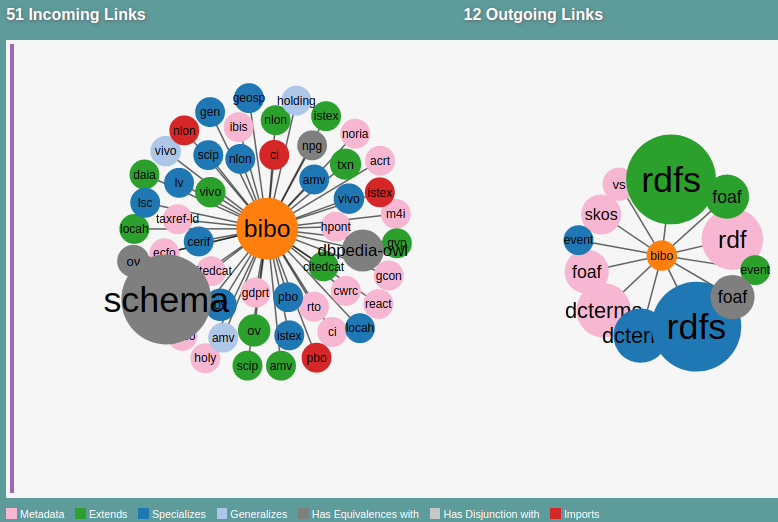
\includegraphics[width=17cm]{BIBO_LOV.png}
    \caption{La place de l'ontologie de domaine \textit{BibO}: à gauche, les ontologies utilisant \textit{BibO}; à droite, les ontologies utilisées par \textit{BibO}. Capture d'écran depuis \textit{Linked Open Vocabularies}, 18 août 2023 (https://lov.linkeddata.es/dataset/lov/vocabs/bibo)}
    \label{fig:enter-label}
\end{figure}


\subsubsection{Structure et granularité}

L'interopérabilité du Web de données ne peut reposer autrement que sur des définitions communes des prédicats. C'est pourquoi ils prennent également une forme d'URI:\\

\large
$$
\underbrace{https://w3id.org/skgo/modsci\#}_{Namespace}\underbrace{hasManufacturer}_{Propri\acute{e}t\acute{e}}
$$
\normalsize

Le \textit{Namespace} (ou \textit{espace de nom}) est une partie de l'URI qui se répètera dans chaque prédicat distinct issu d'une même ontologie. La seconde partie est la propriété, qui apporte la valeur sémantique au prédicat. Dans cet exemple, le prédicat est utilisé pour affirmer qu'une entité (le sujet) a pour fabricant (prédicat) un agent (en objet).\\

Pour minimiser la redondance lors de l'écriture, les \textit{Namespaces} sont régulièrement préfixés. Cela doit être déclaré avant l'utilisation de l'ontologie, bien que la syntaxe dépende du format de sérialisation (\hyperref[annexe-syntaxes]{Voir les exemples en Annexes)}. Pour reprendre l'exemple ci-dessus, il sera le plus souvent formulé de cette manière: 

\large
$$
\underbrace{modsci:}_{Pr\acute{e}fixe}\underbrace{hasManufacturer}_{Propri\acute{e}t\acute{e}}
$$
\normalsize

Les ontologies incluent également une hiérarchisation des propriétés, qui peuvent ainsi répondre avec plus ou moins de granularité à des impératifs d'expression. L'exemple ci-dessous est issu du modèle \textit{CIDOC-CRM} (le modèle conceptuel utilisé par les musées\footnote{\cite{internationalcouncilofmuseumsClassesPropertiesDeclarations2022}})
\begin{center}    
\begin{tabular}{|c|llll|}
\hline
ID du prédicat & \multicolumn{4}{c|}{Nom du prédicat}\\
\hline
P12 & \multicolumn{4}{l|}{occurred in the presence of}\\
\hline
P11 & & \multicolumn{3}{l|}{- had participant}\\
\hline
P14 & & & \multicolumn{2}{l|}{- carried out by}\\
\hline
P22 & & & & \multicolumn{1}{l|}{- transferred title to}\\
\hline
P23 & & & & \multicolumn{1}{l|}{- transferred title from}\\
\hline
P28 & & & & \multicolumn{1}{l|}{- custody surrendered by}\\
\hline
P29 & & & & \multicolumn{1}{l|}{- custody received by}\\
\hline
\end{tabular}\
\end{center}

\subsubsection{Liens logiques entre prédicats}\label{liens-logiques}
L'application des prédicats peut également être enrichie par la symétrie, l'inversion et la transitivité. Ces concepts définissent des liens logiques induits par l'emploi d'un prédicat - liens qui seront ensuite matérialisés par la création d'un second prédicat. De cette manière, il est possible de déduire et de créer de l'information nouvelle, malgré qu'elle n'ait pas été encodée comme telle.\\

La symétrie implique qu'un prédicat liant un sujet et un objet sera aussi applicable en inversant ce même sujet ce même objet. Il représente la réciprocité. Si \textless Personne 1\textgreater{} \textless est contemporaine de\textgreater{} \textless Personne 2\textgreater, alors \textless Personne 2\textgreater{} \textless est contemporaine de\textgreater{} \textless Personne 1\textgreater.\\

L'inversion précise qu'un sujet relié à un objet par un prédicat deviendra l'objet d'un autre triplet, dépendant la logique de l'assertion. Par exemple, si \textless Personne 1\textgreater{} \textless est l'auteur de\textgreater{} \textless Livre 1\textgreater, alors \textless Livre 1\textgreater{} \textless a pour auteur\textgreater{} \textless Personne 1\textgreater.\\

La transitivité est une relation d'appartenance à un ensemble plus large ou plus restreint. Par exemple, si \textless Ville 1\textgreater{} \textless est situé dans\textgreater{} \textless Pays 1\textgreater{} et que \textless Pays 1\textgreater{} \textless est situé dans\textgreater{} \textless Continent 1\textgreater, alors \textless Ville 1\textgreater{} \textless est situé dans\textgreater{} \textless Continent 1\textgreater. 

\subsubsection{Schema.org}

\textit{Schema.org} est un cas à part. Il ne s'agit pas à proprement parler d'une ontologie, mais plutôt d'un vocabulaire organisé de propriétés. Le vocabulaire est mis en place suite à la collaboration de quatre des principaux fournisseurs de moteurs de recherche, à savoir Google, Microsoft, Yahoo! et Yandex.\\

Avec de tels promoteurs, son usage s'est rapidement étendu et l'a élevé au rang de standard. Les pages Web enrichies de microdonnées formulées avec \textit{Schema.org} sont rendues plus visibles lors d'une requête sur un de ces moteurs de recherche\footnote{Voir \cite[p.~87-88]{arnouldModelisationOntologiquePsychologies2021}, ainsi que \cite[p.~83]{mesguichBibliothequesWebEst2017} ou encore \cite[p.~129-132]{bermesWebSemantiqueBibliotheque2013}}. Si cela le rend difficilement contournable en termes d'optimisation de la visibilité sur le Web, il en devient également très générique, étant en mesure de sémantiser aussi bien des données relatives à la structure d'une entreprise qu'à celles d'une recette de cuisine.\\

Cependant, une collaboration entre \textit{Schema.org} et le W3C a amené en avril 2015 à la définition de \textit{Bib.schema.org}. Ce vocabulaire est destiné à étendre la visibilité des données de bibliothèques par rapport au format \textit{Bibframe}, qui, s'il répond bien aux principes du Web de données, reste essentiellement utilisé par les professionnels\footnote{\cite[p.~56-57]{bermesVersNouveauxCatalogues2016}. Voir également \url{https://schema.org/docs/bib.home.html} (visité le 14/08/2023) et \url{https://www.w3.org/community/schemabibex/wiki/Bib.schema.org-1.0} (visité le 14/08/2023).}.\\




\subsection{Les classes}\label{1-classes}

Une \textit{ontologie} se distingue d'un \textit{vocabulaire} dans le sens ou elle ne définit pas uniquement des prédicats: elle réglemente également la nature des sujets et des objets qu'ils peuvent relier. Dans un contexte RDF, les ressources partageant des caractéristiques similaires sont catégorisées selon des classes, qui aident à spécifier ce que représente chaque ressource et comment elles sont liées les unes aux autres.\\

Les classes assurent la pertinence lors de l'utilisation des prédicats et, par extension, permettent la mise en place des \hyperref[liens-logiques]{liens logiques}. Un exemple simple est que, si l'on veut utiliser le prédicat \og est né à \fg, le sujet doit appartenir à la classe \og Personne \fg, et l'objet à celle des \og Lieux \fg. Nous dirons que le \textit{domaine} (\textit{domain} en anglais) doit être une \textit{instance} de classe \og Personne \fg, et que le co-domaine (\textit{range}) doit être une \textit{instance} de classe \og Lieu \fg.\\

Dans notre exemple provenant du \textit{CIDOC-CRM}, l'ontologie précise également l'usage des classes en tant que domaines et co-domaines:
\begin{center}    
\begin{tabular}{|cccc|c|c|}
\hline
\multicolumn{4}{|c|}{Nom du prédicat} & Domaine & Co-domaine\\
\hline
\multicolumn{4}{|l|}{P12 - occurred in the presence of} & \multicolumn{1}{l|}{E5 - Event} & \multicolumn{1}{l|}{E77 - Persistent Item}\\
\hline
 & \multicolumn{3}{l|}{P11 - had participant} & \multicolumn{1}{l|}{E5 - Event} & \multicolumn{1}{l|}{E39 - Actor}\\
\hline
 & & \multicolumn{2}{l|}{P14 - carried out by} & \multicolumn{1}{l|}{E7 - Activity} & \multicolumn{1}{l|}{E39 - Actor}\\
\hline
 & & & \multicolumn{1}{l|}{P22 - transferred title to} & \multicolumn{1}{l|}{E8 - Acquisition} & \multicolumn{1}{l|}{E39 - Actor}\\
\hline
 & & & \multicolumn{1}{l|}{P23 - transferred title from} & \multicolumn{1}{l|}{E8 - Acquisition} & \multicolumn{1}{l|}{E39 - Actor}\\
\hline
 & & & \multicolumn{1}{l|}{P28 - custody surrendered by} & \multicolumn{1}{l|}{E10 - Transfer of Custody} & \multicolumn{1}{l|}{E39 - Actor}\\
\hline
 & & & \multicolumn{1}{l|}{P29 - custody received by} & \multicolumn{1}{l|}{E10 - Transfer of Custody} & \multicolumn{1}{l|}{E39 - Actor}\\
\hline
\end{tabular}
\end{center}


Tout comme pour les prédicats, les ontologies introduisent des hiérarchies de classes: ces dernières sont organisées en super-classes et en sous-classes. Une super-classe transmet ses caractéristiques à ses sous-classes. Si nous prolongeons notre exemple issu du \textit{CIDOC-CRM}: un \textit{Achat} est bien une instance d'une \textit{Acquisition}, qui est elle-même une \textit{Activité, etc.}:

\begin{center}  
\begin{tabular}{|c|lllll|}
\hline
ID de la classe & \multicolumn{5}{|c|}{Nom de la classe}\\ 
\hline
E4  & \multicolumn{5}{|l|}{Period}\\ 
\hline
E5 & & \multicolumn{4}{l|}{- Event}\\
\hline
E7 & & & \multicolumn{3}{l|}{- Activity}\\
\hline
E8 & & & & \multicolumn{2}{l|}{- Acquisition}\\
\hline
E96 & & & & & \multicolumn{1}{l|}{- Purchase}\\
\hline
E9 & & & & \multicolumn{2}{l|}{- Move}\\
\hline
E10 & & & & \multicolumn{2}{l|}{- Transfer of Custody}\\
\hline
E11 & & & & \multicolumn{2}{l|}{- Modification}\\
\hline
E12 & & & & & \multicolumn{1}{l|}{- Production}\\
\hline
E79 & & & & & \multicolumn{1}{l|}{- Part Addition}\\
\hline
E80 & & & & & \multicolumn{1}{l|}{- Part Removal}\\
\hline
\end{tabular}\
\end{center}

\subsection{La sérialisation}
Le RDF n'est pas considéré comme un format. Il s'agît plutôt d'un cadre ou une méthodologie pour structurer et représenter des données. En revanche, la sérialisation du RDF peut être exprimée en divers formats, tels que RDF/XML, Turtle et JSON-LD notamment, qui vont pouvoir être interrogés avec le langage de requête SPARQL. Une expression en format compatible avec RDF et SPARQL constitue le troisième principe de Tim Berners-Lee pour un Web de données.\\

Chacun de ces formats offre une manière différente de représenter les mêmes informations RDF. Le recours à l'un ou l'autre peut dépendre de besoins spécifiques, des contextes d'utilisation... voire des capacités techniques mobilisables. Nous reprenons ci-dessous, les principales caractéristiques de ces formats. Nous avons également joint en Annexes \hyperref[annexe-syntaxes]{des exemples d'écriture}, en reprenant des URI de ressources et de prédicats issus de Wikidata. 

\begin{itemize}
    \item \textbf{Le format RDF/XML} a été le premier à être utilisé pour exprimer des données en RDF. Ce choix s'est initialement imposé de par la notoriété du XML lors de l'apparition de la notion de Web sémantique. Cependant, il a la particularité d'être assez verbeux, et de souffrir d'un encodage chronophage et complexe. Ceci explique sa baisse de popularité, et le développement d'autres formats plus légers\footnote{\cite[p.~70]{vanhoolandIntroductionAuxHumanites2016}}. Les Archives Nationales, déjà grandes utilisatrices du format XML EAD et EAC-CPF, l'utilisent toutefois comme format d'expression de leurs jeux de données rendus disponibles sur GitHub\footnote{https://github.com/ArchivesNationalesFR/Referentiels (visité le 22/08/2023)}. Data BnF permet aussi l'extraction de ses entités en RDF/XML depuis son portail. 
    
    \item \textbf{Le format Turtle} (\textit{Terse RDF Triple Language}) a été développé pour répondre à la lourdeur de RDF/XML. La syntaxe est semblable au langage de requête SPARQL, ce qui renforce son appropriation par les utilisateurs. Elle a été normalisée par le W3C, qui l'inclut dans le développement de RDF 1.1\footnote{\cite{worldwidewebconsortiumRDFTurtleTerse2014}}. Turtle a également été décliné en N-Triples\footnote{\cite{worldwidewebconsortiumRDFNTriplesLinebased2014}}, qui en est une version plus simple mais moins profonde. En plus du RDF/XML, Data BnF permet l'export de ses notices en Turtle. 
    
    \item \textbf{Le format JSON-LD} (\textit{JavaScript Object Notation for Linked Data}) est un format très répandu. Il a l'avantage d'utiliser le format JSON déjà bien implanté dans le milieu du développement informatique, ce qui le rend familier auprès de nombre d'informaticiens. Google considère ce format comme optimal pour son moteur de recherche, et en recommande l'utilisation; il est d'ailleurs à la base de son \textit{Knowledge Graph}. Le format est cependant plus difficilement lisible pour un humain, et peu réutilisable\footnote{\cite[p.~158]{sireWebSemantiquePolitiques2018}}. Il est à noter que JSON-LD n'est pas un format retenu par DBPedia pour inclure un jeu de données dans son \textit{Linked Open Data Cloud}\footnote{\url{https://www.lod-cloud.net/\#subclouds} (visité le 24/08/2023).}. 
\end{itemize}



\section{Un langage de requête spécifique: SPARQL}

Dans l'optique de participer au Web de données, nombre d'institutions ou de services rendent celles-ci disponibles via des \textit{SPARQL Endpoints}. Ces derniers sont les points de diffusion des données, afin de les partager pour enrichir d'autres jeux de données. Ils sont interrogeables avec SPARQL (\textit{SPARQL Protocol and RDF Query Language}).\\

SPARQL est le langage de requête spécifique au RDF, et qui fait d'ailleurs partie du troisième principe énoncé par Tim Berners-Lee pour un Web de données. Son usage a été élévé au rang de recommandation par le W3C en 2013\footnote{\cite{worldwidewebconsortiumSPARQLQueryLanguage2013}.}.\\

Le langage permet d'interroger l'ensemble des triplets constituant une base de connaissances en RDF, selon une syntaxe logique. L'interrogation va porter sur la place que chaque ressource occupe dans le triplet (y compris le prédicat). Il est d'ailleurs possible de mentionner une ressource une première fois en tant qu'objet, et une seconde fois en tant que sujet, pour construire des requêtes complexes qui parcourent le graphe.\\

Le \textit{Wikidata Query Service} offre des exemples et des raccourcis intégrés à la console d'interrogation, ce qui lui permet d'être plus facilement accessible à un non-initié. Il est loin d'être le plus représentatif de la complexité de la syntaxe de SPARQL, \hyperref[obstacle-SPARQL]{qui n'est d'ailleurs pas sans soulever quelques problèmes}. Cependant, dans la mesure où nous n'aspirons pas ici à produire un manuel d'utilisation\footnote{Des introductions aux principes de SPARQL peuvent être trouvées ici: \cite[p.~71-72]{vanhoolandIntroductionAuxHumanites2016} et \cite{maillotApercusRechercheInterroger2014}}, nous allons prendre un exemple qui en est issu, afin de présenter la logique d'expression. La requête suivante cherche les cathédrales de Paris renseignées dans Wikidata: 
\newpage

\begin{figure}[h]
    \centering
    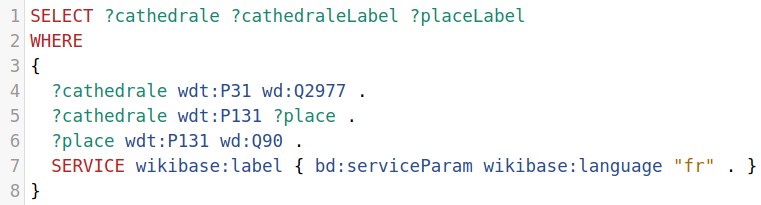
\includegraphics[width=16cm]{SPARQL.png}
    \caption{Exemple d'une requête sur les Cathédrales de Paris dans Wikidata, avec la langue d'affichage des noms courants paramétrée sur le français)}
    \label{fig:enter-label}
\end{figure}
La première ligne indique les résultats que nous souhaitons obtenir lors de la requête: l'URI de la cathédrale (\og ?cathedrale \fg), son nom courant (\og ?cathedraleLabel \fg) et le nom courant de son emplacement (\og ?placeLabel\fg).

La quatrième ligne précise que ce que nous avons posé comme une variable \og ?cathedrale\fg{} a pour nature (propriété P31) une cathédrale (ressource Q2977). 

La cinquième ligne précise que notre variable \og ?cathedrale \fg{} a pour localisation administrative (propriété P131) une variable \og ?place \fg. Nous n'avons pas déclaré directement cette dernière variable en première ligne, mais elle est implicite puisque nous avons demandé son nom courant (\og ?placeLabel\fg). 

La sixième ligne précise que la variable \og ?place \fg{} a pour localisation administrative (propriété P131) Paris (ressource Q90).\\

Le résultat prendra la forme d'un tableau, dans lequel les trois colonnes de résultats correspondent aux trois variables que nous avons demandées en première ligne.
\begin{figure}[h]
    \centering
    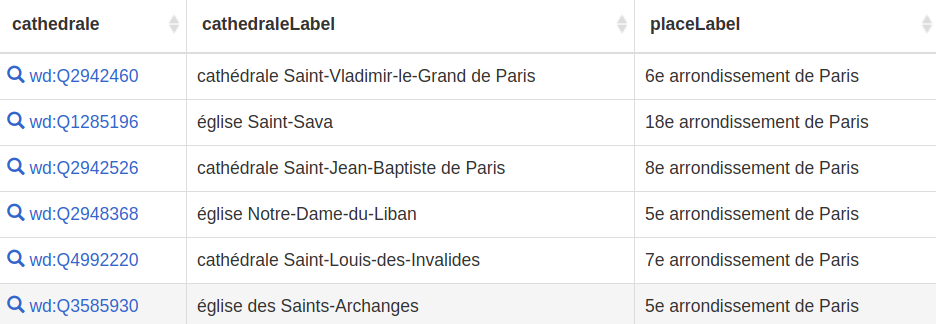
\includegraphics[width=16cm]{RESULTAT_SPARQL.png}
    \caption{Le résultat de notre requête.}
    \label{fig:enter-label}
\end{figure}

Si cet exemple permet de comprendre la logique inhérente à SPARQL, il ne rend pas justice à finesse d'interrogation potentielle offerte par le langage. Interroger le graphe depuis une première entité jusqu'à une dernière entité selon un chemin logique, permet d'interroger des données sur chaque entité intermédiaire. Les opportunités de recherche sont cependant exigeantes, tant en terme de seuil de compétences de l'utilisateur... qu'en termes informatiques, puisque les temps de réponse et montées en charge peuvent être difficiles à assurer pour une machine\footnote{\cite{poupeauAudelaLimitesQue2018}}. 



 
 \part{La pierre angulaire du Web de données: les référentiels}
 

 \chapter{Le référentiel à l'heure du Web de données}\label{referentiel-Wdd}
Nous l'avons esquissé dans les pages précédentes: les technologies du Web de données placent la démarche collaborative au coeur de leur philosophie, à travers les principes des \textit{Linked Open Data} qui encouragent le partage et le réemploi des données. Il n'est de Web de données sans décloisonnement des silos de données, eux-mêmes reflets de processus métiers propres aux institutions. Ce changement de paradigme a également une influence sur la notion de référentiel; constitué initialement de données d'indexation au sein des institutions, il se retrouve à présent défini par son statut de données, au même titre que d'autres jeux de données.\\ 


Apportons également une note terminologique. La rapport final du groupe d’incubation \og Bibliothèques et web de données\fg\footnote{\cite{bakerRapportFinalGroupe2012}} distingue trois types de ressources pouvant créer du lien: les jeux de données (les ressources d'une bibliothèque, tel qu'un catalogue général), les vocabulaires d'autorité (autorités-matière tel RAMEAU, ou autorité-personne tel le VIAF) et les éléments de description de métadonnées (les ontologies). Nous traiterons ci-dessous des deux premiers. 


\section{Une transposition nécessaire}

Dans le vocabulaire interne d'une institution, un référentiel - fût-il un fichier d'autorité, un thésaurus ou un vocabulaire contrôlé - est constitué de données de référence, savamment établi et entretenu par des professionnels pour les besoins d'autres professionnels\footnote{\cite[p.~43]{bermesWebSemantiqueBibliotheque2013}}. Le référentiel répond à un besoin de rationalisation dans l'emploi des termes utilisés au sein d'une institution (lieux, matières, personnes, etc.).\\

Nombre de ces référentiels \og classiques \fg{} ont été transposés dans le Web de données. Leur rôle n'a pas évolué, et ils servent toujours aux processus d'indexation mis en place avant l'arrivée de ces technologies.\\

Ainsi, la BnF a converti ses référentiels internes pour répondre aux besoins d'indexation de Data BnF\footnote{\cite{bibliothequenationaledefranceVocabulairesEmployesBibliotheque2023}}; les notices de RAMEAU\footnote{Pour plus d'informations sur RAMEAU, voir le site web: \url{https://rameau.bnf.fr/} (visité le 28/08/2023).} ont notamment été transposées en URI réutilisables par l'ensemble des bibliothèques qui utilisent ce référentiel pour leur indexation-matière, ce qui inclut notamment les bibliothèques universitaires.\\

Les Archives nationales de France, quant à elles, ont également publié leurs référentiels en 2022\footnote{Voir \url{https://github.com/ArchivesNationalesFR/Referentiels} (visité le 28/08/2023).}, ce qui comprend les référentiels d'agents (personnes physiques, collectivités et producteurs), de lieux et de concepts. Leur projet pilote pour faire rentrer les Archives dans le Web de données a cependant mis en évidence la pauvreté et le relatif abandon de certains référentiels. Ceci est à la fois la cause et la conséquence d'une pratique insuffisante du référencement\footnote{\og En France, [...] on n'indexe pas bien\fg, pour citer Florence Clavaud, en référence au fait que la tradition française s'est essentiellement concentrée sur l'histoire des fonds, des producteurs et des contextes documentaires, plutôt que sur l'indexation et l'enrichissement d'entités contextuelles. Voir \cite[18 min 45 sec] {clavaudRiCAuxArchives2022}}. Les référentiels sont donc toujours en construction, et leur enrichissement fait partie du plan stratégique 2021-2025. 


\section{La transformation de la notion de référentiel}\label{transfo-referentiel}

Si les institutions ne les ont pas abandonné avec l'adoption du Web de données, les \og référentiels \fg{} se sont redéfinis par le changement de modèle apporté par le Web de données. En effet, dans les optiques de réemploi et d'interopérabilité promues par cette technologie, tout jeu de données peut être amené à être réutilisé en tant que référentiel par un tiers, à partir du moment où les données qui le constituent sont d'une qualité estimée suffisante. Il est difficile d'objectiver ce qui distingue des \og données de bonne qualité \fg{} d'autres données; cependant, leur complétude, leur exactitude, leur formalisme, ainsi que la légitimité de son producteur dans le domaine concerné, constituent autant de paramètres qui vont favoriser l'emploi d'un jeu de données comme référentiel\footnote{\cite[p.~43]{bermesWebSemantiqueBibliotheque2013}}.\\

Le nouveau paradigme du Web ne place plus le document au coeur de ses traitements. La fiche cartonnée des bibliothèques et la fiche d'oeuvre des musées sont maintenant découpées en série de données (en attendant d'être rejointes par les inventaires d'archives), qui seront ensuite exploitées et mises en valeur sur le Web. Il en est de même pour les référentiels internes, dont la conversion aux formats du RDF signifie la dilution de leur statut au sein d'un graphe où toutes les entités sont conceptuellement mises sur un pied d'égalité. Tout devient données, et tout jeu de données constitue potentiellement un référentiel.


\section{Vers de nouvelles pratiques}
Si cette mise à plat a remis en question la vision traditionnelle du référentiel, il n'a pas été sans engendrer réflexions et remises en question des modèles préexistants. Ainsi affranchis de leurs distinctions traditionnelles entre données de référence et données opérationnelles, de nouveaux modèles conceptuels ont émergé.\\

\subsubsection{FRBR et IFLA-LRM}

Le secteur des bibliothèques a notamment transformé son modèle. Dès les années 1990, le modèle conceptuel FRBR avait marqué une rupture. En effet, là où les catalogues informatiques consistaient en une version numérique des fiches cartonnées, FRBR distingue à présent les œuvres, expressions, manifestations et items\footnote{Voir les \hyperref[annexe-modconcept]{Annexes}.}, afin de mieux rencontrer les besoins des utilisateurs. Il ne reste malgré tout qu'un modèle conceptuel, et non une application; il faut attendre 2010 et la sortie de RDA (\textit{Resource Description and Access}) pour qu'il soit traduit en normes de catalogage adaptées au Web de données.\\

La fusion (en 2017) de FRBR avec FRAD (pour la rédaction de notices d'autorité) et FRSAD (pour la rédaction des notices d'autorité-matière) accouche d'un nouveau modèle conceptuel: \textit{IFLA-LRM}. Les anciennes données de références de FRAD et FRSAD font désormais partie d'un modèle global, intégré.\\

Ce modèle est à la base du programme de la \og Transition Bibliographique \fg{} porté par la BnF et l'ABES, qui prévoit à la fois l'adaptation de RDA à la bibliothéconomie française (sous la forme de RDA-FR), la migration des données existantes vers ce format de catalogage, et la formation des professionnels à ces pratiques nouvelles\footnote{\cite{bibliothequenationaledefranceProgrammeNationalTransition2023}}.

\subsubsection{CIDOC-CRM}
Le modèle du \textit{CIDOC-CRM} répond en premier lieu à un besoin de modéliser (et donc de mobiliser) la grande variété de sources nécessaires aux musées pour leur documentation. Il se définit comme un modèle capable de décrire des processus et des évolutions en tant qu'entités\footnote{\og As an event-centric model, supporting historical discourse, the CIDOC CRM firstly enables the description of entities that are themselves time-limited processes or evolutions within the passing of time\fg. \cite[p.~33]{internationalcouncilofmuseumsDefinitionCIDOCConceptual2022}}.\\

Ce principe n'est pas sans rappeler le modèle de FRBR puis d'IFLA-LRM, qui s'affranchissent eux aussi d'un modèle de description centré sur la bibliographie. Les points de convergence des deux modèles est d'ailleurs à l'origine du projet \textit{LRMoo}, visant à proposer un modèle d'IFLA-LRM comme une extension du CIDOC-CRM\footnote{\cite{rivaLRMooHighlevelModel2022}}. 

\subsubsection{Records in Contexts}
De son côté, le secteur des archives est également à l'aube d'une profonde mutation. La description archivistique recourt actuellement à quatre standards: 
\begin{itemize}
    \item ISAD(G) pour la rédaction d'instruments de recherche archivistiques à plusieurs niveaux (émise en 1994 et 1999);
    \item ISAAR (CPF) pour la rédaction de notices d'autorité archivistiques relatives aux collectivités, aux personnes et aux familles (1996 et 2004);
    \item ISDF pour la description des fonctions (2007);
    \item ISDIAH pour la description des institutions conservant des archives (2008).
\end{itemize}

\textit{Records in Contexts} (RiC) est une révolution des pratiques archivistiques comparable à la révolution d'IFLA-LRM en bibliothéconomie. La distinction entre données d'autorité et données opérationnelles s'efface au profit d'un seul modèle intégré de production de données. La nouvelle pratique est en cours de définition par l'EGAD (\textit{Expert Group on Archival Description}) depuis 2012; une première version du modèle conceptuel (RiC-CM) en graphe a été publiée en 2016, suivie d'une deuxième version en 2019, et d'une troisième, plus complète, en 2021; la version 0.2 de l'ontologie accompagnant ce modèle (RiC-O) est, elle, publiée en février 2021 pour ouverture à commentaires.\\

RiC est dans le stade final de son développement. Il sera amené à remplacer les quatre standards existants à ce jour, pour faire rentrer les archives dans le Web de données. Les Archives nationales, porteuse du projet pilote, ont néanmoins déjà commencé à convertir leurs données. Ils ont pour cela développé l'outil \textit{RiC-O Converter}, qui transforme les instruments de recherche et notices d'autorités exprimés jusqu'ici en format XML (EAD et EAC-CPF) vers le RDF/XML\footnote{L'outil est téléchargeable sur le dépot GitHub des Archives Nationales: \url{https://github.com/ArchivesNationalesFR/rico-converter} (visité le 29/08/2023).}.  

 
 \chapter{L'interopérabilité et les référentiels}

\section{\og Hub and spoke\fg}
Si la notion de référentiel dans le Web de données tend à se généraliser à tout jeu de données susceptible de produire des ressources en ligne, la conversion en RDF des thésauri, vocabulaires contrôlés et listes d'autorité n'en reste pas moins un facteur d'interopérabilité important. Ils continuent à créer de la convergence entre systèmes différents en agissant \og comme un point nodal ou une colonne vertébrale \fg\footnote{\cite[p.~41]{bermesWebSemantiqueBibliotheque2013}}.\\

Deux institutions vont donc être en mesure de lier leurs ressources par l'emploi d'un vocabulaire commun. La BnF a ainsi converti son plan de classement Dewey en lien vers les URI de ce référentiel; de cette manière, elle peut créer du lien vers les données de n'importe quelle autre institution qui aurait fait de même\footnote{\cite[p.~54]{bermesWebSemantiqueBibliotheque2013}}. 

\begin{figure}[h]
    \centering
    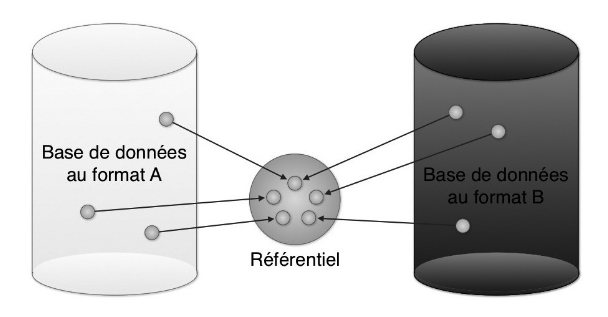
\includegraphics[width=10cm]{ROUE_ESSIEU.png}
    \caption{Illustration de la convergence des données dans un modèle d'interopérabilité \textit{hub and spoke}. Exemple provenant de E. Bermès, G. Poupeau et A. Isaac, \textit{Le Web Sémantique En Bibliothèque}..., p.42}
    \label{fig:enter-label}
\end{figure}


\section{\og Follow your nose \fg}
Toute donnée pouvant être considérée comme un référentiel dans le Web, l'interopérabilité n'est pas uniquement garantie par les référentiels tels que thésauri, vocabulaires contrôlés et notices d'autorité. En effet, une institution peut également privilégier l'emploi d'URI existants pour directement renvoyer vers n'importe quelle entité d'un jeu de données extérieur.\\

Passer de jeu de données en jeu de données au gré des passerelles (les liens) permet un type d'interopérabilité basé sur la navigation intuitive, d'où le nom de \og follow your nose \fg. 

\begin{figure}[h]
    \centering
    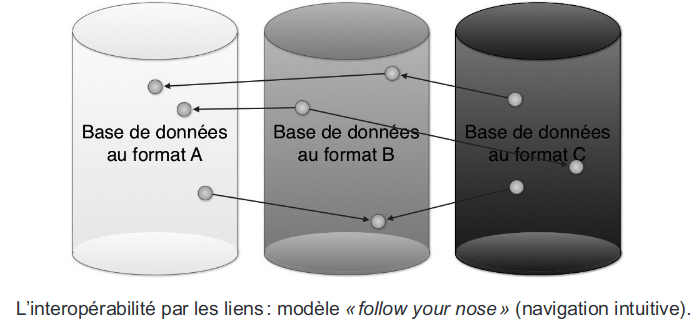
\includegraphics[width=10cm]{FOLLOW_YOUR_NOSE.png}
    \caption{Illustration du modèle d'interopérabilité \textit{follow your nose}. Exemple provenant de E. Bermès, G. Poupeau et A. Isaac, \textit{Le Web Sémantique En Bibliothèque}..., p.42}
    \label{fig:enter-label}
\end{figure}

\section{Au coeur du processus: l'alignement}

Dans l'optique de générer de l'interopérabilité, identifier les ressources équivalentes entre jeux de données devient essentiel. C'est pour cette raison que les institutions mettent en oeuvre des campagnes d'alignement. Des prédicats d'équivalence permettent de décrire de telles relations: \textit{$owl{:}sameAs$} est utilisé pour une équivalence entre deux autorités d'\og individus\fg\footnote{En OWL, \og Individu \fg{} s'entend comme tout ce qui a une identité qui est unique à l'entité. Nous pouvons résumer cela en disant qu'il s'agit de toute entité qui possède un nom propre.}, et \textit{$skos{:}exactMatch$} pour une équivalence entre deux concepts issus d'un vocabulaire contrôlé ou d'un thésaurus.\\

Les Archives Nationales se sont ainsi engagées dans un processus au long cours consistant à apposer des identifiants ISNI dans leurs notices sur les producteurs d'archives\footnote{\cite[p.~86]{clavaudTransformerMetadonneesArchives2019}}. Quant à la BnF, elle s'est alignée sur de nombreux référentiels différents, y compris sur des référentiels internationaux ou étrangers. Le cas de cette institution montre aussi que des alignements peuvent se faire au sein de ses propres jeux de données; en effet, une ressource présentée sur Data BnF peut également se retrouver dans le Catalogue Général et sur Gallica... avec leurs URI distincts.\footnote{\cite{bibliothequenationaledefranceWebSemantiqueModele2023}}\\


\subsubsection{L'alignement des données de l'AAFS}\label{2-alignement-AAFS}

L'alignement peut se faire de façon automatisée, ou bien manuellement. Dans ce dernier cas, c'est un humain qui, sur base de ses connaissances et du contexte de création des données, sera en mesure de déterminer si une ressource est équivalente à une autre. Ce processus peut s'avérer chronophage, mais laisse néanmoins peu de place à l'erreur - sauf cas extraordinairement complexe. C'est de cette manière que les Archives Nationales procèdent pour inclure les identifiants ISNI sur leurs notices, et c'est également ainsi que nous avons procédé, dans le cadre de notre stage, pour récupérer les URI de lieux de production de pièces d'archives depuis le référentiel Geonames.\\

Dans le premier cas, en revanche, l'alignement ne peut se faire de manière satisfaisante que si les données sont suffisamment riches pour réduire l'incertitude au maximum. Ce problème peut survenir lors de la formalisation en RDF d'inventaires qui ont été écrit sous forme textuelle. Notre stage nous a vu procéder de la sorte à trois reprises. Leurs succès contrastés illustrent ces problématiques de qualité des données, et invitent à engager une réflexion sur la manière dont elles sont produites même en dehors d'un contexte RDF:
\begin{itemize}
    \item L'inventaire du patrimoine technique et scientifique comportait des données relatives aux matériaux constituant chaque instrument. Le niveau de détail des composants était généraliste (\og bois \fg, \og métal \fg, ...) et ne rentrait à aucun moment dans de bas niveaux de subdivisions (tels que des bois ou des métaux spécifiques). Les matériaux ont tous trouvé une concordance dans le thésaurus des Techniques de Joconde - thésaurus employé par les musées nationaux pour décrire leurs collections. Ici, c'est l'emploi d'un vocabulaire limité, restreint à l'essentiel, qui a été vecteur de performance.
    \item Pour chaque pièce, l'inventaire du patrimoine artistique et mobilier mentionnait une typologie (\og peinture \fg, \og sculpture \fg, ...), y compris à des niveaux de ramification profonds comprenant des termes très précis (tel que \og facture d'harmonium \fg). En revanche, bien qu'elles n'aient pas été encodées sous forme d'URI, nous avons pu identifier que le moindre de ces termes provenait du thésaurus des Techniques et Domaines utilisé pour la description du Patrimoine Mobilier. Sur base de leur nom, nous avons pu appliquer un script d'interrogation du SPARQL EndPoint\footnote{\url{http://data.culture.fr/thesaurus/sparql} (visité le 01/09/2023)}, et ainsi récupérer les URI pour chaque typologie. Dans ce cas, l'emploi d'un vocabulaire complexe est justifié car celui-ci se repose précisément sur un vocabulaire contrôlé existant, ce qui permet aussi de bon résultats lors de l'alignement.
    \item Dans l'inventaire des bibliothèques, nous trouvions une colonne \og Auteur \fg. Comme nous l'avons mentionné précédemment, l'interrogation de l'API de la BnF a donné relativement peu de résultats. Pour rappel, les auteurs étaient le plus souvent mentionnés sous une forme basique (nom de famille uniquement, éventuellement accompagné d'une initiale de prénom). Nous avons opté pour un compromis entre sécurité et temps de travail, puisque notre script permettait de récupérer l'URI d'un auteur à la condition qu'il soit le seul et unique résultat de la requête. Un contrôle humain a ensuite permis d'estimer qu'ils étaient corrects à 93\%. Les 7\% de données erronées ont été soit corrigées, soit supprimées manuellement. Le reste de la récupération des URI d'auteurs devra se poursuivre à la main. Il est cependant certain que des données initiales plus complètes (avec, à minima, un nom et un prénom complet) auraient permis de collecter plus de résultats. 
\end{itemize}

L'alignement avec un référentiel peut également être impossible, si les données initiales ne s'y prêtent pas. En effet, nous avons rencontré, dans les inventaires d'Archives et de Bibliothèque, des mentions de typologies de documents qui ne correspondent à aucun référentiel existant. Un certain manque de formalisme faisait également apparaître des types d'information similaires dans différentes colonnes des fichiers Excel. La familiarité de ce logiciel, que nous avons tous utilisé à un moment où l'autre de notre vie, peut finalement constituer un obstacle: il nous a tous habitué à prendre des notes \og à la volée \fg, destinées à être lues et comprises par nos collègues. Cependant, cette pratique se rapproche davantage du Web 1.0 et se marie mal avec les principes du Web de données, qui vise précisément à trouver un compromis d'expression entre les langages humain et informatique. Un alignement ne pourra être envisagé qu'après un retravail en profondeur des données.\\

 
\section{L'enrichissement des données}

Lorsqu'un alignement met en évidence l'équivalence de deux URI, nous savons qu'ils font référence à une seule et même chose; dès lors, les assertions formulées pour la décrire dans un système A deviennent transposables dans un système B. Les API et SPARQL EndPoints assument alors leur rôle de portes d'accès vers de nouvelles données, qui peuvent être récupérées et intégrées dans un autre système.\\

\subsubsection{Le cas du référentiel de Lieux des Archives nationales}\label{ref-lieux-AN}

La mise à jour du référentiel de lieux des Archives nationales de France relève, en ce sens, d'un cas d'école. Les 34.000 communes françaises (depuis les années 1940) n'étaient auparavant renseignées que par leur nomenclature et leur département - soit des informations lacunaires. Or, la pauvreté d'un référentiel constitue une menace pour sa pérennité: elle le rend dispensable auprès des utilisateurs, et, par cercle vicieux, leur délaissement ne les place pas au coeur des systèmes d'information\footnote{\cite[p.~72]{clavaudTransformerMetadonneesArchives2019}}.\\

Les Archives nationales ont pu enrichir leurs données de références de lieux en récupérant des données de l'INSEE et de l'IGN. En effet, le premier met à disposition, en accès libre et en RDF, les données du COG (Code Officiel Géographique\footnote{https://www.insee.fr/fr/metadonnees/source/serie/s2084 (visité le 18/08/2023)}) dont elle est productrice. Ce Code décrit les entités administratives françaises avec davantage de précisions, et ses données historiques renseignent en outre les changements de noms, les fusions, etc., qui ont émaillé leur histoire. Après l'alignement des identifiants, les données complémentaires du COG ont pu être versées dans le référentiel de lieux. Les Archives Nationales ont également procédé de la sorte avec les données du second institut, afin de récupérer les coordonnées géographiques des différentes entités administratives - ce qui ouvre de nouvelles opportunités en termes de datavisualisations.\\

Si les Archives Nationales ont pu mettre à disposition un référentiel de lieux pertinent sur GitHub, c'est donc aussi car elles ont été en mesure de constituer un jeu de données conséquent via l'emploi des mêmes technologies\footnote{\cite[49min:15sec]{clavaudRiCAuxArchives2022}}. Ce cas témoigne de la façon dont less jeux de données peuvent se retrouver engagés dans un cercle vertueux d'enrichissement mutuels grâce aux principes du \textit{Linked Open Data}.





 
\chapter{La création de référentiels internes}


\section{Le référentiel interne et le Web de données}

Nous l'avons vu, le Web de données repose sur le principe de créer du lien entre des ressources communes manifestées par des URI. En ceci, le RDF offre un modèle profondément décentralisé, propice aux échanges de données par l'utilisation d'une grammaire commune à un réseau de jeux de données. Dès lors, nous pourrions nous interroger sur la pertinence de créer des référentiels internes. Leur champ d'application se déplace du global au local; cela ne rentre-t-il pas en contradiction avec les principes de décompartimentation des silos du Web de données?\\


Si cela semble être le cas de prime abord, c'est sans compter sur les spécificités du RDF en terme de souplesse syntaxique. Le modèle est en effet très évolutif, taillé pour l'interopérabilité; c'est d'ailleurs son principal intérêt (voire l'\og unique ?\fg\footnote{\cite{poupeauReflexionsQuestionsAutour2018}}). Là où une base de données relationnelle nécessitera une modification de sa structure pour inclure de nouveaux types de propriété/valeur (ou en ajouter de nouveaux), le RDF supportera sans aucun problème l'écriture de nouveaux triplets qui partagent un même sujet ou objet. Ceux-ci se superposent, accumulant ainsi de la connaissance et des références relatives à chaque entité. En ceci, les technologies sémantiques reposent sur la théorie du \textit{monde ouvert}, par opposition au \textit{monde clos} caractéristique d'autres types de bases de données\footnote{\cite{bohnkeVousModelisezMonde2019}}.\\


\subsection{\og Interne \fg, un terme à nuancer}

Le silotage n'est donc pas un critère majeur pour juger de l'adéquation d'un jeu de données avec les technologies sémantiques. Celle-ci sera plutôt tributaire de deux prérequis: un premier, d'ordre technique, selon qu'il soit fidèle aux principes du Web de données énoncés par Tim Berners-Lee ou non; et un second, conditionné par l'application du premier, qui reflètera sa crédibilité en termes conceptuels et méthodologiques.\\

Les quatres principes du Web de données peuvent être résumés comme suit: des URI, formulés avec le protocole HTTP, doivent être sémantiquement liés entre eux selon le modèle RDF et être interrogeables par SPARQL. Une sérialisation en RDF va déjà répondre à deux exigences sur quatre. Les deux restantes peuvent également être remplies si les référentiels sont exprimés sous forme d'URI. Cela signifie que la place d'un référentiel interne dans le Web de données n'est pas dictée par sa nature locale, mais bien par son expressivité. Un référentiel interne à une seule institution est techniquement davantage compatible avec le Web de données s'il est exprimé en URI, qu'un référentiel commun à plusieurs institutions dont il n'existe aucune expression en URI.\\

Comme nous l'avons signalé précédemment, le Web de données accepte potentiellement tout jeu de données comme données de référence. Si les principes énoncés par Berners-Lee sont remplis, la localité ou la globalité d'un référentiel ne va non pas être dicté par des contraintes techniques, mais bien par son adoption et son réemploi par d'autres acteurs. \hyperref[transfo-referentiel]{Nous en revenons à la notion de \og qualité \fg{} des données} qui, bien qu'elle soit subjective, sera déterminante pour déterminer si un référentiel interne peut prétendre à devenir le référentiel externe d'une institution tierce. \\


\subsection{L'enrichissement comme finalité}

L'éventualité que les entités d'un jeu de données ne puissent être exprimées sous forme d'URI n'est pas non plus synonyme d'exclusion totale du Web de données. En effet, la mise en place d'une API ou d'un SPARQL Endpoint va permettre à d'autres institutions de venir interroger et extraire ces données locales. De cette manière, un référentiel interne peut également contribuer aux processus de partage et d'enrichissement mutuel permis par cette technologie. 

 
\section{Les avantages d'un référentiel interne}\label{2-referentiel-int}
Quelque soit sa place au sein du Web de données (URI ou non), un référentiel interne bien utilisé peut constituer un apport significatif à un jeu de données. 

\subsection{Pallier l'absence d'URI}
La première raison est probablement la plus évidente: l'entité n'est présente dans aucun référentiel externe, et, en conséquence, aucun URI n'est disponible pour l'identifier. Les collections patrimoniales peuvent en effet faire intervenir des agents, des sujets ou des lieux très spécifiques, et dont les champs d'évolution peuvent être très éloignés des domaines généraux couverts par les principaux pourvoyeurs d'URI. Cela est d'autant plus vrai pour les fonds d'archives. La création d'une entité de référence devient donc le seul moyen d'émettre des affirmations à propos d'une entité que l'on estime importante pour la compréhension des collections.\\

La notion d'\og importance \fg{} - quoiqu'elle aussi subjective - n'est pas à négliger. Créer une entité n'est effectivement pas automatique dès lors que les ressources n'existent pas dans les référentiels externes. La pertinence du choix peut-être évaluée selon plusieurs critères: quelle place occupe la potentielle entité dans les collections? Est-il nécessaire de le désambiguïser? Est-il intéressant de formuler des assertions à son sujet afin de la documenter? Est-il prévu de lui donner une visibilité par l'éditorialisation? Est-elle amenée à être citée régulièrement\footnote{En ceci, les questions sont similaires à la question de création - ou non - d'URI pour identifier ses ressources. Voir: \cite[p.~3]{ministeredelacultureetdelacommunicationIdentifiantsPerennesPour2014}}? Ces questions peuvent finalement être résumées en une seule: est-ce utile?\\


\subsection{Proposer une contextualisation pertinente}
Un référentiel interne peut ne pas être composé exclusivement de ressources inédites. Décrire des entités ayant une correspondance externe en même temps que des entités uniquement locales constitue une opportunité pour émettre des affirmations utiles à la contextualisation des données dans leur ensemble. Adapter la description à des besoins documentaires spécifiques apporte une consistance et une pertinence supplémentaire au jeu de données. L'impératif sera alors de créer du lien d'équivalence (via les prédicats {$skos{:}exactMatch$} et {$owl{:}sameAs$}) entre les ressources du référentiel interne et leurs équivalents existants.\\

Cette pratique peut contourner un des revers des grands référentiels. En effet, les référentiels externes peuvent se montrer individuellement inadaptés, car les descriptions peuvent ne pas suffire à contextualiser un projet spécifique. Ainsi, dans le cas de Marc Seguin (qui constitue notre entité la plus solidement référencée), l'information est fractionnée, incomplète et redondante: Wikidata reprend des données biographiques génériques (dates de naissance, de décès, lieu d'inhumation, éducation, etc.), tandis que VIAF et l'ISNI ne reprennent que les données de la BnF relatives aux ouvrages dont il est l'auteur. Le seul apport réel de ces référentiels externes consiste en l'établissement d'un vocabulaire controlé, distinguant les formes retenues et rejetées du nom. Ils ne peuvent à aucun moment prétendre à atteindre le degré de complétude et d'interconnexions de référentiels internes constitués dans le seul but de documenter ses activités.\\


\subsection{Proposer une grille de lecture nouvelle}\label{2-grille-lecture}

La création d'un référentiel interne peut également être au coeur de la définition d'un projet, en matérialisant des approches originales et des grilles de lecture nouvelles envers des jeux de données qui auront été retravaillés - voire recomposés, en usant des opportunités de réemploi des données offertes par le RDF - en ce sens. Ils peuvent servir de point nodal à la constitution de corpus destinés à favoriser la construction d'un discours de recherche ou de médiation.\\

Le cas des archives d'ethnologues à la bibliothèque Éric-de-Dampierre est, à ce titre, un bon exemple de la construction d'un discours de recherche. Bien que les scientifiques n'avaient pas constitué leurs corpus de travail selon cette méthode, un nouvel axe de présentation des fonds a permis de réorganiser et de présenter les documents d'archives sur base de la mission de recherche lors de laquelle ils ont été produit\footnote{\cite[p.~18]{carbonnelArchivesSciencesHumaines2017}}. Le recours à un référentiel organisé et utilisé de façon systématique peut donc servir un propos scientifique, original et construit.\\

Le processus d'indexation thématique des inventaires des collection de l'AAFS relevait, lui, partiellement du processus de médiation. Si le référentiel met en lumière des thématiques scientifiques, certains termes ont été établis en vue de faciliter la diffusion d'éléments de médiation tels que le processus d'autoformation et d'éducation scientifique chez les Seguin. 



\section{La création de référentiels à l'AAFS}
Dans le cadre de notre stage, nous avons procédé à la création de plusieurs jeux de données de référence. Ceux-ci ont servi à l'indexation des collections, dont la mise en base des différents inventaires constituaient un des aspects principaux de la mission.\\

Nous avons ainsi créé: 
\begin{itemize}
     \item Un jeu de données de référence de personnes: le jeu de données contient 59 entités, dont l'essentiel décrivent des membres de la famille Seguin (à des degrés plus ou moins éloignés). D'autres sont des collaborateurs dont les noms apparaissent régulièrement dans les archives, ou dont l'importance historique est jugée plus importante.
     \item Un jeu de données de référence des agents collectifs, soit essentiellement des entreprises et sociétés savantes ayant marqué l'histoire des Seguin ou de leurs activités. Ce jeu de données contient 26 entités.
     \item Un jeu de données de référence sur les ouvrages et contributions scientifiques de Marc Seguin, comprenant 20 entités. A cet égard, nous avons choisi d'appliquer le principe de l'\textit{IFLA-LRM}, qui place l'oeuvre comme une entité à documenter au même titre que son émanation (c'est-à-dire une publication spécifique). 
     \item Un petit jeu de données de référence de Lieux, contenant 4 entités. Ces lieux (Saint-Marc, Varagnes, le Laboratoire de Varagnes et l'Observatoire de Varagnes) sont profondément liés aux activités des Seguin et au domaine qui sera mis en valeur par la constitution de la Fondation.
     \item Un jeu de données d'indexation matière, comprenant 59 entités. Ce jeu de données est amené à mettre en lumière des thématiques spécifiques rencontrées au sein des différentes collections, afin de former des ensembles consultables par l'utilisateur. 
\end{itemize}

\subsection{Une constitution postérieure aux inventaires}

La démarche de création des référentiels internes à l'AAFS est particulière, dans le sens où ces données n'ont pas été créées lors de la constitution des différents inventaires, mais bien après.\\

Le choix des entités à décrire ne s'est pour autant pas fait à notre discrétion uniquement. En effet, l'AAFS avait produit une liste de termes à mettre en évidence à travers les collections: personnes, sociétés, thématiques scientifiques, techniques et sociales, lieux, typologies de documents... Les archives avaient précédemment été consultées, mais cette liste n'est pas le fruit d'un dépouillement méthodique des fonds. Cette méthode n'est pas sans incidence sur le résultat de l'indexation, avec de grandes disparités d'occurences d'un terme à l'autre.\\

Notre opération de consultation des fonds a néanmoins permis de confronter cette liste de termes avec la réalité des indexations. Nous avons été en mesure de l'affiner et de désambiguïser certains termes, en collaboration avec le responsable scientifique.\\

En revanche, la définition progressive des entités de référence a entraîné de fréquents va-et-vients dans le processus d'indexation. L'apparition d'une nouvelle entité nous a amené a revoir à plusieurs reprises la liste des documents, afin de procéder à une indexation rétroactive. Il n'est pas exclus que l'exhaustivité en ait été la première victime.  



\subsection{L'impact d'un manque de référentiel interne}

Dans nos pages, nous avons présenté les possibilités d'interopérabilité offertes par le Web de données à travers l'emploi des référentiels communs. Cependant, le rôle premier d'un référentiel utilisé en interne est de structurer la production de données. Le manque de référentiel interne amène ainsi à deux constats.\\

Premièrement, dans le cas ou plusieurs inventaires sont produits par des prestataires différents - comme c'est le cas pour les inventaires de Varagnes -, cela se traduit par l'emploi de normes, graphies, etc., propres à chacun. Les différents inventaires en viennent donc aisément à référencer une même ressource de manière différente.\\

Deuxièmement, lors de la constitution d'un inventaire, une même personne peut également utiliser différentes appellations différentes pour désigner une même entité conceptuelle. Dans certains cas, cela peut s'expliquer par le fait qu'une graphie ou un nom d'auteur peut être une information historique en elle-même (l'évolution de la signature d'une personne, l'emploi d'un pseudonyme d'écrivain, etc.); cependant, la plupart des cas relevaient plutôt d'une difficulté à retrouver les précédentes manifestations d'un nom, et par conséquent d'en adopter une graphie unifiée. Le manque de référentiel ne conduit pas, dans ce cas, à un défaut d'interopérabilité avec d'autres inventaires, mais bien à générer une information confuse au sein d'un seul. \\

Le principe de l'indexation a donc nécessité une mise en forme unifiée pour chaque occurence, opérée manuellement. Cela a également permis de régler de nombreux problèmes d'ambiguïté de termes: notre référentiel de personnes contient trois \og Marc Seguin \fg, de même que trois \og Paul Seguin \fg, deux \og Louise Seguin \fg, \og Louis Seguin\fg, \og Joseph Seguin \fg{} et \og Augustin Seguin \fg; quant aux agents collectifs, nous avons pu en désambiguïser certains noms, pour mieux en refléter la signification au fur et à mesure des nombreuses fusions et transformations (\og Buire\fg, \og Forges de l'Horme\fg{} tout particulièrement).\\

Si l'opération ne pose pas de problèmes de faisabilité majeurs, elle n'en reste pas moins extrêmement chronophage. Les opérations d'inventaire futurs pourront, en revanche, se baser sur nos référentiels et faire des économies de temps de travail. La structure de données est également mise en place, ce qui facilitera la création de nouvelles entités de référence.


\subsection{Une contextualisation optimale}

Comme nous l'évoquions précédemment, les référentiels internes permettent de proposer une contextualisation en cohérence avec la nature du projet. Dans le cas de notre stage, nous avons appliqué ce principe en mettant l'accent sur le dialogue constant entre eux, afin de tisser un réseau de relations dont la multiplicité et la diversité des noeuds reflète des pans de l'histoire familiale des Seguin, ainsi que de l'histoire de l'industrie, du capitalisme familial du XIX\textsuperscript{e} siècle, ou encore des sciences. 

\begin{itemize}
    \item Les personnes ont été reliées à d'autres personnes (parents/enfants, conjoints, relations de travail), aux agents collectifs (fondateurs, directeurs, employé), aux ouvrages (auteur) et aux lieux (de naissance, de décès).
    \item Les agents collectifs ont été reliés aux personnes (fondateurs, directeurs, employés) et à d'autres sociétés (fusion, refondation)
    \item Les ouvrages ont été réliés aux personnes (auteurs)
    \item Les lieux ont été reliés aux personnes (lieux de naissance, de décès)
\end{itemize}
\bigskip
Quant au processus d'indexation des pièces d'inventaires, il s'est effectué selon ces divers axes: 
\begin{itemize}
    \item Les personnes ont servi à l'indexer: 
    \begin{itemize}
        \item Archives: les producteurs et les destinataires de correspondance;
        \item Art et mobilier: le créateur d'une oeuvre;
        \item Bibliothèque: l'auteur d'un ouvrage.
    \end{itemize}
    \item Les agents collectifs ont permis d'indexer:
    \begin{itemize}
        \item Les archives qui documentaient leurs activités;
        \item Les pièces du patrimoine scientifique et industriel produites par elles.
    \end{itemize}
    \item Les ouvrages de Marc Seguin ont permis d'indexer les pièces d'archives selon qu'il s'agisse de travaux préparatoires, d'exemplaires édités, ou de documents apportant des informations générales;
    \item Les thématiques ont été utiles à tous les inventaires, à l'exception de la Bibliothèque, pour laquelle les délais de la mission ne permettaient pas de procéder à une indexation sur des quantités de documents aussi vastes;
    \item Les lieux ont servi à indexer les pièces d'archives selon leur lieu de production.
\end{itemize}


 
	\part{Appréhender un projet d'entrée dans le Web de données}


Le Web de données a été adopté par de nombreuses institutions patrimoniales, et leurs réalisations servent aujourd'hui de points de repère pour évaluer les apports du Web de données. Ce sont d'ailleurs les plus grandes institutions qui ont défini de nouveaux modèles conceptuels, de nouveaux langages et de nouvelles normes, afin de rendre leurs données publiques selon cette nouvelle donne éditoriale. Pour ce faire, elles se sont basées sur une longue tradition documentaire, et sur d'importants moyens humains, techniques et financiers.\\

Cependant, toutes les institutions ne bénéficient pas d'une telle longévité et de telles ressources. Pour celles-ci, entrer dans le Web de données peut s'avérer plus complexe encore que pour les grandes: adopter des standards qui n'ont été ni définis par eux ni adaptés à leurs propres activités, faire rentrer dans le moule du RDF des données disparates, ou encore être relativement coupés de l'expertise développée par les services compétents. Pour ces plus petites structures, il peut y avoir un gouffre entre la théorie et son application.\\


Notre stage à l'AAFS s'intègre dans ces réflexions. Les huit inventaires à notre disposition, créés par de nombreuses personnes aux expériences diverses, ont dû être normalisés pour répondre à des modèles stricts. Nous avons également dû créer des référentiels internes, afin de contextualiser l'information. En ce sens, il s'est avéré très formateur.\\

L'AAFS a choisi Omeka-S pour rentrer dans le Web de données. Depuis 2017, ce logiciel - \textit{open source}, donc gratuit - se destine à faciliter l'entrée dans le Web de données, notamment en proposant une interface de création de bases de données en RDF qui dispense de la moindre connaissance préalable en RDF/XML, Turtle/N3 ou en JSON-LD. Le logiciel permet également une éditorialisation aisée. Pour ces avantages, il a été adopté pour de nombreux projets\footnote{Voir par exemple une liste des sites créés avec Omeka-S: \url{https://omeka.org/s/directory/} (visité le 31/08/2023)}.\\


Les considérations que nous développerons ci-après reflètent les questionnements, obstacles et préoccupations que nous avons rencontrés au cours de notre stage, que ce soit vis-a-vis d'Omeka-S ou de façon plus générale envers le Web de données. Elles s'inscrivent dans une mise en perspective sur ce qu'implique l'entrée dans le Web de données pour une petite institution, tant en termes de gestion de projet que d'opérations à effectuer sur les données. Nous souhaitons également souligner quelques contraintes et limites du Web de données, afin qu'une institution puisse appréhender quelques-un des défis posés par cette technologie. A chaque fois que cela se révèlera nécessaire, nous présenterons également comment Omeka-S se positionne vis-à-vis de la question soulevée. \\


\chapter{La solution Omeka-S}

\section{Présentation}

Omeka-S est un logiciel destiné à la mise en ligne de fonds d'archives, d'éditions numériques et de bibliothèques numériques, selon un formalisme similaire aux principes du \textit{Linked Data}. Omeka-S n'est pas appelé à remplacer le logiciel initial Omeka (appelé à présent \og Omeka Classic \fg{} afin de marquer la différence entre les deux versions). Il s'agit davantage d'une \og réécriture\fg{} de celui-ci, destinée notamment aux institutions qui gèrent plusieurs sites Web\footnote{\cite{OMEKA2016}}. La première version d'Omeka-S est lancée en novembre 2017. Il se veut être une solution mêlant simplicité et polyvalence.\\

La mise en ligne des ressources se fait à travers l'alimentation d'une base de données fonctionnant en arrière-plan du site; celle-ci est donc invisible à l'utilisateur. Chaque ressource ainsi insérée est automatiquement éditorialisée sur le site Web lié à la base\footnote{Pour peu qu'elle ait été paramétrée comme telle lors de sa création en base de donnée. Cependant, cette option est celle retenue par défaut.}, et répond au formalisme du RDF, dans le sens où elle est décrite par l'affichage des triplets dont elle est le sujet et l'objet.\\

Notons cependant que l'affichage en RDF n'est pas synonyme de l'écriture selon l'un de ses formats dans la base de données. Omeka-S fonctionne sur la pile logicielle LAMP, pour Linux (système d'exploitation), Apache (serveur), MySQL (base de données relationnelle) et PHP (langage de programmation). Le stockage des données suit donc le modèle relationnel, bien que l'interface de travail soit créée de sorte que cela ne se ressente pas.\\

En plus des pages Web décrivant les ressources, Omeka-S permet de créer des pages Web \og classiques \fg, dont le contenu est alimenté essentiellement sous format textuel par un humain. La création de ces pages est simplifiée, de sorte qu'aucune compétence en modélisation de page Web (HTML ou CSS) n'est requise: l'écriture se fait via un éditeur, qui va offrir une interface semblable à celle d'un logiciel de traitement de texte standard. En cela, nous pouvons dire qu'il inclut un CMS (\textit{Content Management System}, dont \textit{WordPress} est aujourd'hui l'exemple le plus connu). La création de pages Web sous cette forme peut néanmoins inclure des composantes plus complexes, via l'insertion de ressources décrites en base de données, de médias, de fenêtres renvoyant du contenu d'un autre site, etc.\\ 


\section{Fonctions de base}

Nous ne présenterons pas en détail le fonctionnement du logiciel, qui n'a, pour l'essentiel, que peu d'importance à notre propos et relèvent des principes généraux du Web de données. Les entités d'Omeka-S prennent le nom d'\textit{item}. Ces items peuvent être rassemblés en une (et une seule) collection, dont le terme employé est \textit{item set}. Des \textit{medias} peuvent également être liés aux items et item sets.\\

Le logiciel vient avec quelques ontologies préinstallées, sélectionnées parmis les ontologies essentielles du RDF: \textit{SKOS}, \textit{Dublin Core Terms}, \textit{BibO} ou encore \textit{Friend of a Friend}. Des ontologies supplémentaires peuvent bien sûr être installées, en renseignant l'espace de nom et le préfixe, ainsi qu'en insérant le vocabulaire dans le système.\\

Ces fonctionnalités basiques permettent de créer autant d'item que nécessaire. La page d'un item affichera, par défaut, tous les triplets pour lequel l'item actif est le sujet. Un onglet permet de visualiser les triplets dont l'item actif est l'objet.\\

Une fonctionnalité remarquable est la possibilité de définir des \textit{resource templates}, qui agissent en quelque sorte comme des formulaires reprenant une série de prédicats qui y auront été compilés préalablement. Cela permet de s'assurer que toutes les entités seront décrites de la même manière: ainsi, un \textit{template} peut être utilisé pour décrire les agents, un second pour les pièces d'archives, un troisième pour les lieux, etc. Si cela facilite énormément la mise en place de la base de données, les avantages sont encore supérieurs en termes de transmission et, par extension, de pérennité, puisqu'ils garantissent un maintien des schémas de modélisations de données au fil du temps. Nous avons joint \hyperref[modelisations-AAFS]{en Annexes} les modélisations de données réalisées pour l'AAFS, ordonnées selon le type d'entité.\\


Le logiciel tire également parti de \textit{modules}\footnote{\url{https://omeka.org/s/modules/}, visité le 31/08/2023.}. Ils agissent comme des extensions des fonctionnalités de base. Il y en a des dizaines, et leur nombre augmente au fur et à mesure que de nouveaux sont créés ou que des fonctionnalités d'Omeka Classic sont adaptées à Omeka-S. Nous avons pu en utiliser quelques unes lors de notre stage: \textit{CSV Import} (alimentation de la base par CSV), \textit{Numeric} (pour entrer des dates dans le système selon la norme ISO 8601), \textit{Inverse Properties} (pour définir des \hyperref[liens-logiques]{prédicats inverses}), \textit{Bulk Export} (exports \hyperref[3-exportsOS]{sous différents formats)}, ...



\section{La place d'Omeka-S dans le Web de données}\label{omeka-dans-wdd}
Sur la page d'accueil de son site Web, Omeka-S se présente comme une solution pour se \og connecter au web sémantique \fg\ et pour \og publier [ses] ressources avec des \textit{Linked Open Data}\fg{} \footnote{https://omeka.org/s/ (visité le 19/08/2023)}. La modélisation des données en RDF tend à confirmer cette affirmation, mais elle mérite néanmoins quelques commentaires.\\



Omeka-s remplit effectivement une partie du principe du Web de données: à partir de la page d'une ressource, il est effectivement possible de \og parcourir le graphe \fg{} en naviguant vers une autre, de manière instinctive et ergonomique. Cependant, il s'en éloigne de manière fondamentale du fait qu'aucune des pages qu'il génère ne constituent un URI. Prenons cet exemple (issu des ressources de l'AAFS):

\large
$$
\underbrace{https://epotec.univ-nantes.fr/s/seguin/}_{Corps}\underbrace{item/3970}_{Identifiant}
$$
\normalsize

Cet adressage n'est pas pérenne. En effet, l'\og Identifiant \fg{} ne reflète pas un identifiant immuable de la ressource, mais bien l'ordre d'écriture dans la base de données sur laquelle se repose le site Web. L'identifiant est donc une variable, appelée à être modifiée en cas de migration vers une nouvelle installation d'Omeka-S. Dans ce cas, un lien tel que présenté en exemple deviendra un lien mort.\\

En ceci, les ressources décrites par Omeka-S sont les \og noeuds blancs \fg{} que nous avons mentionnés précédemment. Ils sont bel et bien inclus dans le graphe de connaissances, mais leur portée ne dépasse pas le cadre local.\\

Ce constat place Omeka-S dans une position hybride dans le Web de données: les données bénéficient de ses capacités d'éditorialisation, mais ne pourront pas constituer un référentiel utilisé par une institution tierce - faute de garantie de pérennité des liens. Elles ne répondent pas au premier principe du Web de données tel qu'énoncé par Tim Berners-Lee. Les bases de données d'Omeka-S sont donc placées hors de portée d'une mise en réseau de bases de données liées, tel DBPedia.\\

En revanche, Omeka-S peut toujours mettre ses données à disposition à travers son API, afin de constituer un réservoir dans lequel une autre institution viendrait récupérer des données qu'elle juge intéressantes. 




\chapter{Le Web de données face à la pratique}


\section{Quelques généralités}

\subsection{Les implications en termes de données}

Le Web de données peut être adopté pour de nombreuses raisons: ses avantages incluent l'ouverture des données, les enrichissements potentiels, une modélisation riche et la mise en relation avec des données émises par de grandes institutions. Si ces opportunités résonnent comme des arguments en faveur du modèle, il s'agit en revanche d'une technologie exigeante, et dont certaines de ces caractéristiques avantageuses sont tempérées par des contreparties.\\

Les points soulevés ci-dessous ne constituent pas une liste de prérequis, dont il faut cocher toutes les cases avant de pouvoir accoucher d'un projet pertinent. Ils ont plutôt pour objectif d'inviter à la réflexion, afin de déterminer si le Web de données est la technologie la plus appropriée à un projet d'éditorialisation. 



\subsubsection{Un partage total des données?}\label{3-confidentialite}
C'est l'une des caractéristiques fondamentales des \textit{Linked Open Data}: les données sont destinées à être rendues visibles, et potentiellement récupérables par quiconque, indépendamment des usages potentiels.\\

Cependant, certaines données doivent rester confidentielles. La publication de certaines entités peut par exemple attenter à des contraintes légales (droit d'auteur, respect de la vie privée), éveiller des problématiques de sécurité (publier des emplacements physiques d'objets, ou des visuels permettant la forgerie) ou encore susciter tensions et incompréhensions (les fonds privés peuvent notamment faire resurgir des \og affaires de famille \fg{} sensibles).\\

Ces questionnements sont tout à fait légitimes, mais doivent être anticipés. L'important sera alors de déterminer quelle proportion de données sera ou non publiable, et d'être en mesure de visualiser l'intérêt d'un jeu de données ainsi épuré. Si les données sont par trop dénaturées, le Web de données n'est peut-être pas une solution adéquate.


\subsubsection{Les données liées comme essence du modèle}
Créer du lien entre entités constitue tout l'attrait de cette technologie. Certaines grandes réalisations (Data BnF, Wikidata, Isidore, ...) en présentent une version aboutie, où l'interopérabilité de type \og follow your nose \fg{} permet une expérience enrichissante pour l'utilisateur en passant de lien en lien.\\

Cependant, nous avons également vu que les objets d'un triplet peuvent être exprimés sous format textuel à la place d'URI. Ce sont des éléments importants de la description d'une entité... mais un recours trop important à un tel format d'écriture au sein d'un jeu de données peut nuire à la navigation intuitive, qui constitue pourtant l'un des points forts du modèle et un facteur d'interopérabilité.\\

Il s'agit donc à la fois d'analyser ses données, non seulement pour estimer leur potentielle expressivité sous forme d'URI ou de noeuds blancs, mais également pour déterminer dans quelle mesure des indexations par référentiels internes pourrait leur apporter de la plus-value.


\subsubsection{Tirer parti de l'évolutivité}
La modélisation riche et complexe entre entités est également l'une des caractéristiques du RDF. Cet avantage est à placer en étroite relation avec un autre: la souplesse du modèle d'écriture, qui tolère bien mieux les ajouts que d'autres modèles de base de données (SQL et XML en tête). L'expressivité du RDF est ainsi mise en valeur au fur et à mesure que les jeux de données s'accroissent et se complexifient. Malgré ses exigences techniques, le RDF est un modèle dynamique par excellence.\\

En ce sens, faire rentrer ses données dans le moule sémantique constitue également une opportunité de les faire évoluer. \hyperref[ref-lieux-AN]{Comme le cas du référentiel de Lieux des Archives nationales a pu le démontrer}, le modèle RDF peut d'ailleurs constituer une réponse à un jeu de données pauvre - et ainsi résoudre d'éventuelles faiblesses en lien avec les deux points précédents.\\

Si cette perspective peut s'avérer alléchante, elle implique également la définition de nouveaux projets d'extractions de données, d'alignements, ou de toute autre démarche allant vers l'enrichissement. Le Web de données encourage les processus d'enrichissement à long terme.\\

Il n'est bien sûr pas obligatoire de procéder de la sorte, mais cela revient à se priver d'un des points forts de la technologie. Un jeu de données appelé à rester figé peut, éventuellement, se prêter à une modélisation selon l'hypothèse du \og monde clos \fg{} et être modélisé en base de données plus simple à maintenir que les modèles ayant recours au RDF\footnote{\cite{bohnkeVousModelisezMonde2019}}. 
 



\subsection{L'accès à la compétence}\label{3-competence}

Un paramètre essentiel dans un projet de Web de données est la question de la compétence. En effet, les opportunités offertes par le modèle RDF n'ont que peu été adoptées par les organisations autres que celles du domaine patrimonial, malgré qu'elles aient suscité une vague d'engouement certain à leurs débuts.\\

Ainsi, tandis que les grandes sociétés de l'IT ont, dans l'ensemble, adopté le modèle du \textit{Property Graph}\footnote{\cite{poupeauBilan15Ans2016}}, le modèle RDF a pu être critiqué pour sa complexité et sa lourdeur\footnote{\cite{cagleWhySemanticWeb2016}}, ses problèmes en termes d'ingéniérie structurelle et de sécurité\footnote{\cite{targetWhateverHappenedSemantic}}, de performance de requête après un déploiement à grande échelle\footnote{\cite{poupeauTechnologiesWebSemantique2018}}, voire d'à présent \og mordre la poussière \fg{} face aux opportunités offertes par le \textit{Machine Learning}\footnote{\cite{cabedaSemanticWebDead2017}}. Les principes du modèle ont nourri de nombreuses réflexions opérationnelles en même temps qu'ils ont apporté de nouveaux formats à présent plus répandus; cependant, leur application générale résonne comme un semi-échec, et, hormis dans des secteurs spécifiques, s'essouflent.\\

En conséquence, la maîtrise des technologies sémantiques est moins répandue que d'autres, et de la formation sera probablement nécessaire pour rendre une équipe de travail opérationnelle. La mise en place du \textit{Système de préservation et d'archivage réparti} (SPAR) a ainsi nécessité une mise à niveau technique chez le personnel des organisations participantes, Atos et la BnF\footnote{\cite{poupeauTechnologiesWebSemantique2018}}. Les équipes de la bibliothèque Éric-de-Dampierre ont également du recourir à un formateur pour faciliter la prise en main d'Omeka\footnote{\cite[p.~17]{carbonnelArchivesSciencesHumaines2017}}. La question a également été soulevée pendant notre stage, puisque nous seuls possédions quelques connaissances théoriques et techniques sur l'application des technologies sémantiques.\\

L'accès à des compétences techniques ne relève pas uniquement de la mise en place d'un système, mais également de son évolutivité et de sa pérennité. Celles-ci sont complètement dépendantes de la capacité d'une institution à s'approprier une part de la technologie dans ses termes les plus vastes: la logique fondamentale, ses requis en termes de données, ses possibilités et ses limites, ainsi que tout le vocabulaire qui y est lié.\\

Notons que, de ce point de vue, Omeka-S répond à ses objectifs d'accès simplifié. Si cela ne dispense aucunement de connaître les principes fondamentaux du RDF, il permet de s'affranchir de la moindre écriture en format XML/RDF, JSON-LD ou autre Turtle, grâce à l'ergonomie de son interface.\\



\section{Traiter ses données}

Une institution entrant dans le Web de données va se trouver tôt ou tard face à des questions pratiques de mise en forme de ses données, afin de répondre à ses principes de définitions communes de vocabulaires et de ressources. 


\subsection{La sélection des données}

\hyperref[3-confidentialite]{La question a déjà été abordée sous l'angle de la confidentialité}, mais elle touche ici à une question technique et de pertinence éditoriale. Qu'est-il nécessaire d'éditorialiser?\\

Rien n'empêche de publier l'ensemble de ses données, quitte à ce que certaines soient également exprimées au sein de jeux de données externes. La redondance n'est pas un problème en soi. Au contraire, une institution met en valeur l'unicité historique de ses collections et, par leur éditorialisation, est en mesure de marquer sa spécificité et de gagner en visibilité. La mise en place d'entités de référence - dont quelques-unes peuvent être redondantes - permet d'ailleurs une contextualitation appropriée et de présenter de nouveaux axes du discours, \hyperref[2-referentiel-int]{comme nous l'avons vu précédemment}. \\

Dans ce cas, la priorité va aller vers l'établissement de liens entre ressources identiques\footnote{\cite[p.~69-70]{bermesWebSemantiqueBibliotheque2013}}. Si cela peut sembler, de prime abord, une contrainte importante, nous pouvons aussi y voir des opportunités: un inventaire de bibliothèque renvoyant à des notices bibliographiques du Catalogue Général de la BnF pourra se reposer sur les numérisations rendues accessibles par Gallica, par exemple.\\

Les thésauri, vocabulaires contrôlés et fichiers d'autorités reconnus ne doivent, en revanche, pas être transposés tels quels. Reproduire ces grands ensembles dans un graphe de connaissance local n'apporte aucune plus-value, et il convient de les renseigner sous leur forme d'URI.\\


\subsection{La transposition en URI}

\hyperref[2-alignement-AAFS]{Nous avons soulevé ces questions avec l'alignement}, mais elles constituent un enjeu majeur de l'analyse préalable des données.\\

En effet, transformer ses données vers le modèle RDF implique de créer du lien entre les données initiales (établies sous forme textuelle) et les entités qu'elles représentent sur le Web de données (établies sous forme d'URI). Si le volume de données est faible, l'alignement peut être fait manuellement par une personne qui en aura été chargée. Si les risques d'erreur en sont considérablement réduits, cela nécessite néamoins un temps de travail non négligeable, qui doit être considéré dans le planning du projet.\\


Dans le cas d'un volume important, une récupération automatisée des correspondances peut s'avérer préférable. Bien qu'elles aient été créées en format texte, des termes peuvent être issus de référentiels externes; il convient alors de les identifier ou d'interroger le producteur de l'inventaire à ce sujet.\\

Certaines compétences informatiques seront spécifiques pour aligner les données initiales avec des URI existants, dont la capacité à (apprendre à) interroger des \textit{SPARQL EndPoints} ou des \textit{API REST} mis en accès libre. La bibliothèque \textit{Requests} pour Python est également essentielle, afin de sérialiser les requêtes et de les exporter en formats de données directement adaptés à un import en masse. Le logiciel \textit{Postman} peut également fournir une aide pour tester des requêtes et comprendre leur logique, avant de les formuler avec Python. 



\subsection{Créer ou recréer de la donnée structurante}

Chaque entité d'une modélisation en graphe est distincte et unique. Sa description ne se fait que via les triplets qui l'ont pour sujet ou objet. Elle est ainsi coupée de l'environnement documentaire dans lequel elle avait pu évoluer auparavant - tel qu'un inventaire numérique ou une base de données relationnelle - et notamment les informations de classement et de hiérarchie. Elle devient autonome. Les ensembles plus vastes à laquelle elle appartient sont pourtant des informations de contextualisation.\\

Cela est particulièrement vrai pour les archives, dont les instruments de recherche sont le fruit d'une expertise qui met en perspective le document et son producteur selon un ordonnancement cohérent. Pour reprendre les termes de Laure Carbonnel, un \og travail de fragmentation et de réassemblage d'entités \fg{} au profit de la seule et unique indexation par référentiel \og [effacerait] la spécificité du document d'archives \fg\footnote{\cite[p.~18]{carbonnelArchivesSciencesHumaines2017}}.\\

Le modèle conceptuel des bibliothèques - FRBR puis IFLA-LRM - s'est précisément affranchi du modèle unique de description d'entités matérielles seules, en introduisant les notions d'\textit{Oeuvre}, \textit{Expression} et de \textit{Manifestation} avant d'en être améné à décrire l'\textit{Item}. À la différence d'un inventaire d'archives, \hyperref[mod-ifla-lrm]{cet arbre \textit{OEMI}} n'est pas une hiérarchie, car les attributs de chaque entité ne s'appliquent pas à l'entité suivante; en revanche, il matérialise la volonté de créer des ensembles intermédiaires regroupant les différentes éditions, afin de faciliter l'accès à l'information notamment pour l'utilisateur\footnote{\cite{bibliothequenationaledefranceProgrammeNationalTransition2023}}.\\

Ces exemples montrent que les graphes - et les données qu'ils modélisent - peuvent inclure des noeuds structurants, non pas destinés à l'indexation mais à apporter de la lisibilité à un ensemble trop vaste d'entités coupées de leur substrat d'origine. \\

Convertir un inventaire en RDF ne se limitera donc pas aux pièces qu'il décrit: (re)construire une structure est essentiel à la contextualisation d'une information. Il peut également être nécessaire de recourir à de l'information disséminée dans plusieurs fichiers. Par exemple, l'inventaire du patrimoine artistique de l'AAFS consistait en un tableur simple, mais les pièces décrites ont été liées à d'autres entités représentant les collections et sous-collections qui avaient été établies dans un rapport annexe en PDF. 



\subsection{Créer son ontologie?}
L'analyse des données peut mettre en évidence des situations où aucun prédicat ne semble approprié pour décrire tout ou une partie d'une ressource. La question de créer une ontologie adaptée à ces besoins peut alors de poser.\\

De manière générale, il est conseillé de se passer de cette option au maximum. Les ontologies sont en effet un vecteur d'interopérabilité important, puisque ce sont elles qui vont ordonner des données selon leurs valeurs sémantiques; une ontologie personnalisée ne sera pas intéropérable - à moins, bien sûr, qu'elle ne réponde à un besoin exprimé simultanément par plusieurs institutions dans le cadre d'un projet commun.\\

Cette remarque s'applique d'autant plus en cas d'utilisation d'Omeka-S: si le module \textit{Custom Ontology} permet de créer sa propre ontologie, y avoir recours diminuera la capacité du jeu de données à être extrait par l'API... Capacité qui, pourtant, constitue le seul élément qui le relie au Web de données, eu égard de \hyperref[omeka-dans-wdd]{l'incapacité du logiciel à émettre les prédicats en dehors du contexte local}.\\

Les données problématiques pourrait éventuellement être retravaillées, afin qu'elles s'adaptent à des précidats existants:
\begin{itemize}
    \item Des données peuvent être mises en commun, pour peu que l'ensemble ainsi formé soit cohérent avec la nature de la description. Ainsi, dans le cadre de notre stage, nous avons fusionné différents champs de mesure (\og hauteur \fg, \og largeur \fg, \og profondeur \fg{} et \og diamètre \fg) sous une seule valeur. Nous n'avons en effet pas trouvé d'ontologie qui offrait des prédicats distincts pour chacune.
    \item Des données peuvent être extraites d'un champ, si l'état initial entraîne une dilution de la valeur sémantique d'un prédicat. Par exemple, un champ \og Titre \fg{} de notre inventaire de Bibliothèque pouvait également contenir des mentions d'édition ou de nombre de volumes. Nous avons séparé les valeurs concernées selon des prédicats de \og Titre \fg, \og Edition \fg{} et de \og Nombre de volumes \fg{} distincts. 
\end{itemize}


\chapter{Surmonter quelques limites du Web de données}


\section{L'affirmation et la standardisation en sciences humaines}
Comme nous l'avons vu, la structure du modèle RDF repose sur la formulation d'assertions à l'aide de triplets, reliant entre eux deux entités dont l'expression est standardisée sous la forme d'un URI. Les réalisations du Web de données telles que Data BnF, Isidore, ou encore DBPedia démontrent que le modèle est applicable à de larges jeux de données factuelles. Mais qu'en est-il des informations qui ont besoin de davantage de contextualisation pour être complètes ou valables? Un modèle affirmatif peut-il s'appliquer sans limite aux sciences humaines? 

\subsection{La mise en contexte d'un triplet}
L'usage d'un triplet s'exprime sous forme brute, sans nuance. Il suppose qu'une assertion est forcément vraie et acceptée par tous. Cependant, les sciences humaines regorgent d'exemples où une information est à nuancer. Ainsi, quel degré de certitude peut-on associer à une affirmation? Qui l'a formulée? S'applique-t-elle à de façon unique et constante au sujet?\\

En d'autres termes, il est déjà possible de contextualiser une entité par les liens, mais il est plus complexe de faire de même au niveau du triplet. Aurélien Bénel le déplore lorsqu'il souligne la disparition de la subjectivité dans la modélisation du Web sémantique\footnote{\cite{benelArchivesNumeriquesConstruction2017}}. S'il existe bel et bien des solutions, une institution devrait estimer le degré de contextualisation nécessaire à ses données, car aucune n'est parfaite.\\


\subsubsection{La réification}\label{3-reification}
La réification consiste à considérer un triplet comme une entité identifiée par un URI (ce qu'elle n'est pas), que l'on pourrait contextualiser en la plaçant dans un autre triplet - en vue de préciser son type, son degré de certitude, ou une date d'application, par exemple. Cela se traduit par l'ajout d'une ligne dans l'écriture du triplet, comme spécifié dans la recommandation du W3C sur le RDF.\footnote{\cite{worldwidewebconsortiumRDFSemanticsReification2004}}\\

Cependant, cette option n'est pas sans défaut. Il n'est ainsi pas possible d'ajouter plus d'un attribut au triplet initial, ce qui limite la profondeur de la contextualisation. Il affecte également la fluidité du parcours du graphe et brouille la place du triplet dans celui-ci. Pour ces raisons, l'usage de cette méthode n'est pas recommandé\footnote{\cite{poupeauQuelEvenementOu2010}}.\\

C'est pourtant une mécanique qu'Omeka-S a adopté avec ses \textit{annotations}. Un triplet peut même en recevoir plusieurs. Cependant, il s'agit là d'une solution propre au logiciel, et qui ne pourra être réimplantée telle quelle dans un autre système. En effet, un export de données en JSON-LD marquera cette annotation par l'attribut \og @annotation \fg, alors que celui-ci n'existe pas dans la syntaxe standard de JSON-LD. De plus, si l'annotation est bel et bien visible sur la base de données, elle ne le sera pas sur le site Web, ce qui réduit encore l'intérêt de la fonctionnalité.\\
 \begin{figure}[h]
    \centering
    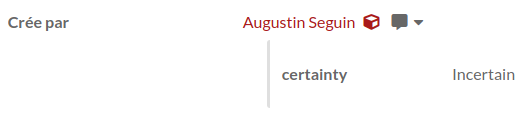
\includegraphics[width=10cm]{annotation_OS.png}
    \caption{Visualisation d'une annotation dans Omeka-S.}
    \label{fig:enter-label}
\end{figure}

Notons cependant que, parmis les grands référentiels structurés par RDF, seul Wikidata se démarque. Fidèle à l'esprit d'identification des sources déjà appliqué à Wikipédia, la plateforme a introduit le référencement chaque information, apportant ainsi une touche de contextualisation à ses triplets. 

\subsubsection{La \og modélisation orientée Évènement\fg}\label{mod-evenement}
La modélisation orientée Évènement\footnote{Voir à ce sujet \cite{poupeauQuelEvenementOu2010}} implique une modélisation particulière, consistant à traiter un évènement comme une entité propre, pouvant être documentée par autant de triplets que nécessaire.\\

La modélisation CIDOC-CRM, utilisée dans le milieu muséal, en est un exemple. Elle introduit une couche de granularité supplémentaire en donnant aux évènements une place centrale. Cela sert tant pour la documentation historique que pour la documentation métier. L'ICOM reprend régulièrement l'exemple de Winckelmann et du Groupe du Laocoon\footnote{Que nous reproduisons en \hyperref[model-cidoc-crm]{Annexes}}, mais nous utiliserons un exemple comparatif simplifié:
 \begin{figure}[h]
    \centering
    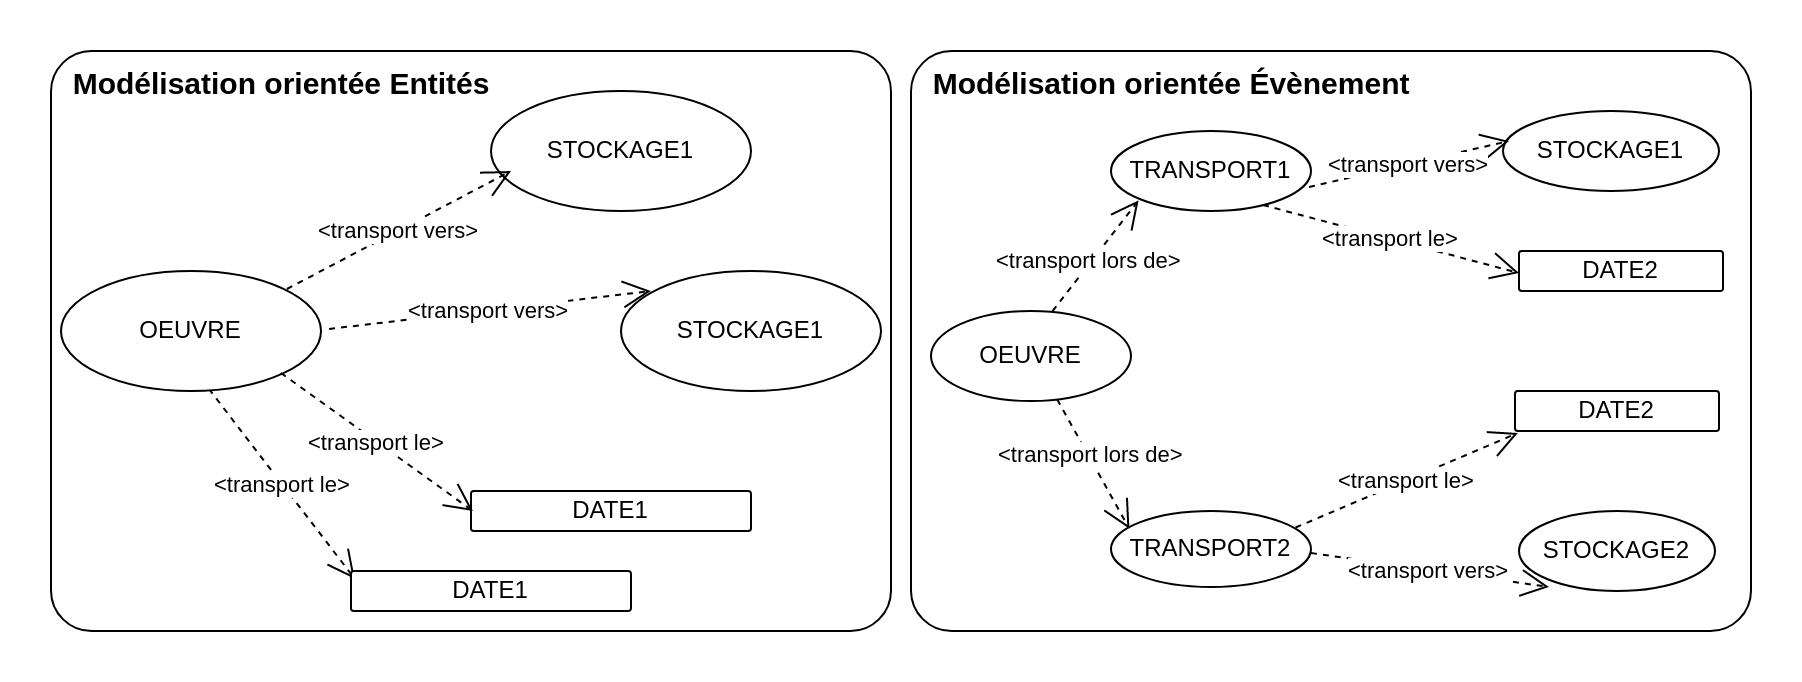
\includegraphics[width=16cm]{EVENEMENT.png}
    \caption{Dans cette comparaison, nous voyons qu'une modélisation orientée Entités (à gauche) montrerait rapidement ses limites en termes de lisibilité de l'information: quelle date se rapporte à quel transport? En utilisant la modélisation orientée Évènement, de nouveaux noeuds sont ajoutés pour décrire plus finement les réalités opérationnelles de l'institution.}
    \label{fig:enter-label}
\end{figure}

Le CIDOC-CRM propose une grande variété de classes relatives aux Évènements, comme nous l'avons montré dans la \hyperref[1-classes]{section sur les classes}. Les ontologies \textit{The Event Ontology}\footnote{\url{https://motools.sourceforge.net/event/event.html} (visité le 28/08/2023).} et \textit{Linking Open Descriptions of Events}\footnote{\url{https://linkedevents.org/ontology/} (visité le 28/08/2023)} peuvent aussi être utilisées pour modéliser des évènements.\\

Notons également que l'ontologie \textit{Dublin Core Terms} contient une classe Évènement. Bien que la modélisation que nous avons produite pour l'AAFS ne soit pas orientée Évènement, nous y avons eu recours pour instancier les voyages de membres de la famille en tant que thématique.\\

Ce type de modèle se distingue par sa finesse. Les principes de la modélisation orientée Évènements peuvent techniquement être appliqués à n'importe quel sujet. Par exemple, une base de données de toponymie pourrait créer un évènement de type \textless reçoit le nom\textgreater{} pour chaque occurence, lui permettant de contextualiser son emploi. Le revers de la médaille est l'alourdissement considérable du graphe. Ce type de modélisation doit donc être pensé dès la définition du projet, tant dans la définition des objectifs que dans l'analyse des données initiales.\\

Dans la mesure où cette option ne fait que rajouter des noeuds à un graphe, elle est tout à fait applicable dans Omeka-S, après chargement des ontologies concernées. 

\subsection{Le nommage des entités}
Nous avons vu que le RDF suppose une appellation unique pour désigner une ressource. Son nom devient alors une valeur figée. La gestion de la synonymie par la constitution de thésauri et de vocabulaires contrôlés en est une application avantageuse; en revanche, dans le cas de noms propres, cela constitue une standardisation qui peut faire perdre de l'information.\\

Ainsi, par exemple, la notice du romain \textit{J'irai cracher sur vos tombes} telle que présentée sur Data BnF\footnote{\url{https://data.bnf.fr/ark:/12148/cb15078920b} (visité le 25/08/2023).} propose un lien vers la page de Boris Vian. Si cette dernière reprend bien \textit{Vernon Sullivan} parmi les nombreux pseudonymes de l'auteur, le lien n'est pas réalisé sous cette forme.\\

Les métadonnées archivistiques doivent également recourir à des formulations standardisées, bien que les usages de l'époque puissent être riches en information (évolution de noms de lieux, de personnes, de titres, ...). L'équipe de Laure Carbonnel a choisit la solution d'user de différents prédicats pour distinguer l'expression d'époque de l'expression standardisée pour des archives d'ethnographes\footnote{\cite[p.~18-19]{carbonnelArchivesSciencesHumaines2017}}. Il s'agit effectivement de la solution à privilégier, même si, comme elle le souligne elle-même, cette formulation historique secondaire ne répondra pas aux standards d'échanges de données. 

\section{Le réemploi des données}
\subsection{L'obstacle de SPARQL}\label{obstacle-SPARQL}

La réutilisation des données est le pilier de l'\textit{Open Data} et du Web de données: la mise à disposition des données leur permet d'être partagées au plus grand nombre, et sans restriction d'usage. La problématique du \hyperref[3-competence]{manque de compétences techniques} vient cependant mettre à mal ce principe.\\

En effet, nombre d'institutions ayant adopté ces technologies se sont dotées d'un \textit{SPARQL EndPoint}, afin de permettre à chacun d'interroger le \textit{triplestore} et ainsi de récupérer les données souhaitées. En revanche, si SPARQL permet des interrogations extrêmement fines, la maîtrise peu répandue de ce langage de requête constitue un frein à leur réemploi. Pour avoir été régulièrement en contact avec les chercheurs, Raphaëlle Lapotre, ancienne cheffe de produit à la BnF actuellement responsable de projets numériques à l'EHESS, rapportait en 2017 ce problème d'accès à l'information\footnote{\cite[1h 35min 40sec]{banat-bergerQuelRenouvellementFormes2017}}:
\begin{quotation}
    \og On entre surtout en contact avec les chercheurs quand ça se passe mal avec les données... et ça se passe souvent mal [...] Pour plusieurs raisons. Mais, effectivement, il y a eu la question de ces fameux standards, qui bouffent la vie des chercheurs [...] Souvent, ils nous disent: "Mais pourquoi vous balancez pas des CSV, plutôt que de vous embêter à faire du Web sémantique...? Et puis le SPARQL, c'est inutilisable, et puis vos données, on ne comprend rien". \fg
\end{quotation}

Même s'il peut être attendu des chercheurs qu'ils \og s'adaptent \fg{} ou cherchent assistance\footnote{\cite[1h 41min]{banat-bergerQuelRenouvellementFormes2017}} dans leurs requêtes, beaucoup vont renoncer et se replier vers des jeux de données accessibles... quitte à réemployer toujours les mêmes, tant qu'ils ne sont pas exprimés en RDF. L'ouverture totale des données, bien que réelle sur le principe, en devient toute théorique. Clarisse Bardiot, chercheuse en Humanités Numériques, va même jusqu'à parler d'une \og certaine hypocrisie sur la soi-disant accessibilité des données via les APIs\fg\footnote{\cite{bardiotHappyAPIsDebridons2018}.}.\\

Une institution souhaitant publier ses données en \textit{Linked Open Data} devra tenir compte de cet état de fait - qui n'est malheureusement pas amené à évoluer - si l'ouverture des données constitue l'un des objectifs essentiels de son projet. A tout le moins, elle pourrait être amenée à développer les compétences de son personnel, afin d'être en mesure de porter assistance à un chercheur dans ses requêtes. 

\subsection{L'accès aux données depuis Omeka-S}

Omeka-S propose des solutions différentes selon le statut de l'utilisateur: un visiteur n'aura accès qu'au site Web et l'API, tandis qu'un administrateur aura également accès à la base de données sous-jacente. La mise en place de l'API n'ayant pas fait partie de notre stage, nous ne sommes aptes à n'en présenter que les possibilités théoriques.

\subsubsection{Depuis le site Web}
Le module \textit{Advanced Search}\footnote{\url{https://omeka.org/s/modules/AdvancedSearch/} (visité le 01/09/2023)} d'Omeka-S permet l'insertion, à partir du CMS, d'un formulaire de recherche standard pour explorer la base de données. La page Web ainsi générée dispose de plusieurs champs de recherche, tel que la recherche libre, par collection, par classe ou par \textit{resource template}, ainsi que selon les valeurs Titre, Auteur, Créateur, Sujet, Date, Description et Classe d'une entité. Une recherche par intervalle temporel peut affiner les paramètres de recherche.\\

Si cette solution offre la visualisation à un utilisateur, elle ne propose pas d'export sous un quelconque format.


\subsubsection{Depuis l'API}
Le logiciel propose un service d'API (\textit{Application Programming Interface}) qui permet de générer des opérations CRUD (\textit{Create}, \textit{Read}, \textit{Update}, \textit{Delete}) sur la base de données. Elle peut être déployée de deux manières (dans un environnement PHP\footnote{Voir \url{https://omeka.org/s/docs/developer/api/php\_api/} (visité le 31/08/2023)} ou via une API REST\footnote{Voir \url{https://omeka.org/s/docs/developer/api/rest\_api/} (visité le 31/08/2023)}).\\

Dans le premier cas, le résultat de la requête sera exprimé en PHP. Dans le second, il sera exprimé en JSON-LD. Des formats plus répandus (type tableur) ne semblent pas disponibles, ce qui signifie que l'utilisateur aura besoin de compétences techniques poussées pour traiter les données exportées. 

\subsubsection{Depuis la base de données}\label{3-exportsOS}
Le module \textit{Advanced Search}, qui offre déjà une interface de recherche pour l'utilisateur sur le site Web, peut également être utilisé sur l'interface de la base de données. Afin de répondre à des besoins d'administrateur, la finesse des requêtes est plus poussée: outre les possibilités déjà mentionnées, il permet d'interroger la base selon des propriétés, la présence de médias, la visibilité, par identifiant, ... Le résultat sera une liste d'\textit{items} (d'entités) répondant au critères de recherche.\\

Le module \textit{Bulk Export}\footnote{\url{https://github.com/Daniel-KM/Omeka-S-module-BulkExport} (visité le 01/09/2023)} permet d'extraire des données depuis l'interface de la base de données. Les données exportées dépendent de ou des ressource(s) active(s) - (liste d')\textit{items}, (liste d')\textit{item sets}, ou médias. Le format du fichier d'export peut être un fichier JSON (JSON ou JSON-LD), un tableur (CSV, ODS ou TSV) ou encore en texte simple (TXT). Les exports sous tableurs ou fichiers texte ne peuvent traiter l'export des \hyperref[3-reification]{annotations}.\\

Notons que l'export sous un format JSON-LD est le seul moyen d'obtenir une représentation générale du graphe de la base de données. Cela disqualifie encore un peu plus les données issues d'Omeka-S pour rejoindre le réseau de données de DBPedia - qui, pour rappel, n'accepte pas ce format. Cependant, la \hyperref[omeka-dans-wdd]{variabilité des identifiants} d'entités d'Omeka-S constituait déjà un obstacle difficilement surmontable.\\

De manière générale, Omeka-S ne semble pas proposer de solution radicalement innovante pour favoriser l'export des données, dont les modalités constituent pourtant un talon d'Achille du Web de données.
       
	
	
	\chapter{Conclusion}

A travers ce mémoire, nous avons présenté le Web de données sous des aspects divers: historiques, conceptuels, fonctionnels et opérationnels. Notre stage à l'AAFS a permis d'illustrer certaines problématiques inhérentes à l'adoption de cette technologie à la fois complexe et contestée, mais porteuse de promesses fortes.\\

Le temps n'est cependant plus aux promesses. Le Web de données a maintenant atteint suffisamment de maturité pour faire face à ses faiblesses, mais aussi à ses avantages. Peut-être ne rencontrera-t-il jamais le niveau d'exigence que certains ont pu attendre de lui, mais il est devenu une réalité pratique. Ses contributions aux performances des moteurs de recherche et à l'établissement de gigantesques bases de données collaboratives ont assurément marqué une période de l'histoire d'Internet et du Web. Le modèle a prouvé qu'il pouvait fonctionner, bien que ses caractéristiques n'ont pas forcément rencontré les intérêts et exigences des grands acteurs économiques.\\

Si les espoirs n'engagent que ceux qui les ont conçus, la technologie se heurte, de manière beaucoup plus pragmatique, à des contraintes fortes dès qu'il s'agit de la mettre en oeuvre. Peut-être n'est-ce pas un hasard si elle a notamment trouvé un relais bienvenu dans les institutions patrimoniales. Leur longue tradition professionnelle en ont fait des producteurs de données par excellence - qui plus est de données historiques et documentaires, plus stables et pérennes. Leurs missions de divulgation et de soutien à la recherche les prédisposent aussi à engager des réflexions sur les moyens de mettre leurs données à disposition, tout en étant, sans en être complètement affranchies, moins soumises aux retours sur investissements qui peuvent diriger le monde économique.\\

S'engager dans un projet de valorisation de collection avec les technologies du Web de données peut se révéler impressionnant. Une institution candidate voit rapidement émerger face à elle une quantité de questionnements, de concepts et de modèles qu'il n'est pas aisé d'appréhender. Elle ne bénéficiera pas des mêmes moyens humains et financiers que celles qui l'ont précédée au niveau (inter)national. Elle ne bénéficiera pas forcément non plus de la même qualité pour ses données initiales, résultat de missions ponctuelles plutôt que de processus affinés pendant des décennies ou des siècles.\\

Pour ces institutions, Omeka-S leur est apparu comme une porte d'entrée bienvenue. Il est gratuit, est soutenu par une communauté importante, et surtout, il se positionne comme une solution logicielle mettant l'accent sur la simplicité. Omeka-S dispense effectivement de parties non négligeables du savoir faire technique requis, notamment en termes d'écriture dans les formats traditionnels du RDF. Mais développer son propre modèle d'entrée dans le Web de données ne se fait pas sans sacrifices. En effet, le logiciel souffre de faiblesses qui le place dans une position hybride, adoptant les opportunités éditoriales du Web de données, sans être en mesure ni d'assumer des fonctions essentielles au modèle en terme de pérennité, ni de résoudre la problématique de la complexité du requêtage.\\

Les avantages et désavantages d'Omeka-S ne sont pour autant pas toute la clef du problème. Même sous une forme simplifiée, le Web de données est exigeant quant aux typologies et à la qualité de ses données. Une institution peut rapidement se trouver face à des problèmes de normalisation et d'alignement de ses données avec des jeux de données d'autorité. Elle peut certes éditorialiser ses données telles quelles avec Omeka-S; mais ne pas s'aligner sur les prérequis du modèle la fait probablement passer à côté de son essence même.\\

Notre mémoire s'inscrit dans cette réflexion. En présentant les principes du Web de données, nous avons fait référence aux grandes réalisations, aux projets qui ont abouti. Ces principes, énoncés en lien avec leur application idéale, représentent les possibilités offertes par la technologie. Nous avons cependant cru nécessaire de contrebalancer cette vision, en la confrontant aux réalités auxquelles des institutions plus modestes doivent faire face. Non pas pour en dresser un portrait au vitriol, comme tant d'autres ont pu le faire, mais pour partager des questionnements et réflexions, dans l'optique de faire avancer un projet et, \textit{in fine}, de participer à son développement. 



 
	\addcontentsline{toc}{chapter}{Conclusion}
	
	%les annexes
	\appendix
        \chapter{Linked Open Data Cloud}

        
\begin{figure}[h]
    \centering
    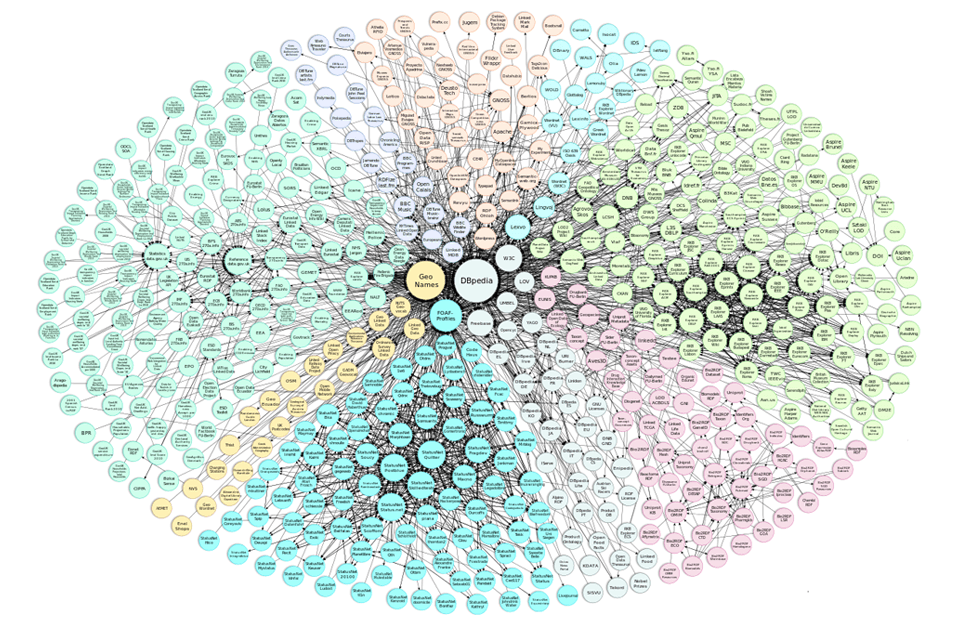
\includegraphics[width=22cm, angle=90]{linked_open_data_cloud.png}
    \caption{Le réseau de données connectées sur le \textit{Linked Open Data Cloud}, initié par DBPedia}
    \label{fig:enter-label}
\end{figure}
 
        \chapter{Quelques modèles conceptuels}\label{annexe-modconcept}
 \begin{figure}[h]\label{mod-ifla-lrm}
    \centering
    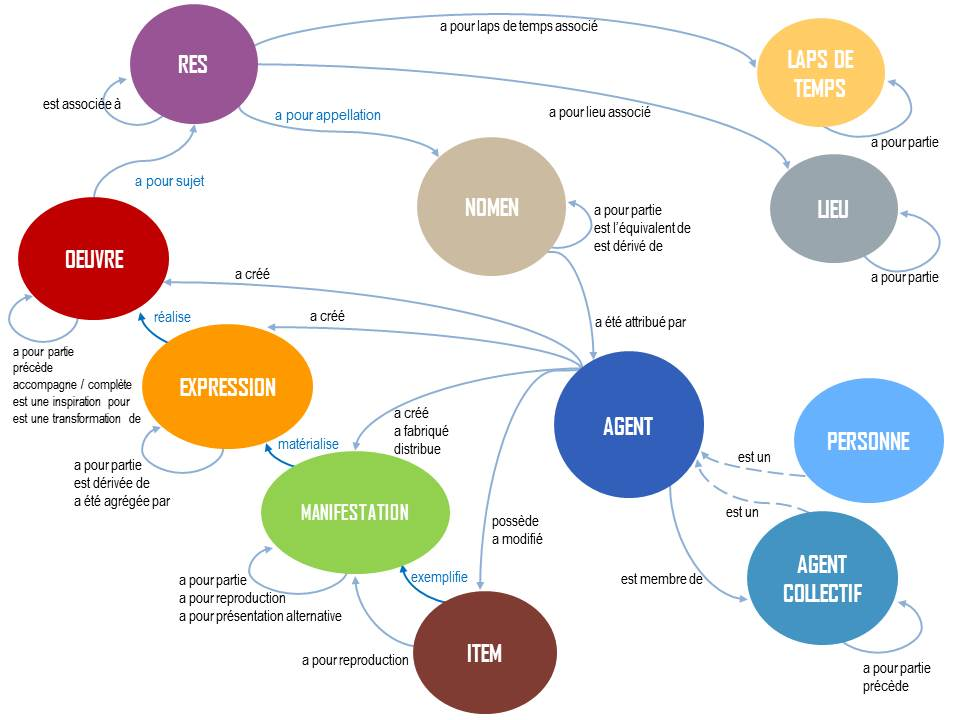
\includegraphics[width=16cm]{Schema_LRM.jpg}
    \caption{Modèle conceptuel IFLA-LRM (\textit{IFLA - Library Reference Model}). Il est le résultat de la fusion (dès 2010) de trois modèles distincts développés précédemment par l'IFLA: FRBR (notices bibliographiques) FRAD (notices d'autorités) et FRSAD (notices d'autorités matière). Cette modélisation est au coeur de la \textit{Transisition Bibliographique}; elle se distingue des méthodes de catalogage traditionnel par la prépondérance de l'oeuvre intellectuelle sur l'objet matériel (constitué par le livre). L'arbre OEMI se décompose en Oeuvre (l'oeuvre telle qu'imaginée par son créateur), qui se réalise à travers une Expression (une traduction, une adaptation, ... de l'oeuvre), elle-même matérialisée par une Manifestation (le contenu intellectuel issu de l'Expression), elle-même exemplifiée par l'Item (le livre physique). Voir https://www.transition-bibliographique.fr/enjeux/definition-ifla-lrm/ (visité le 25/08/2023)}
    \label{fig:enter-label}
\end{figure}



\begin{figure}[h]
    \centering
    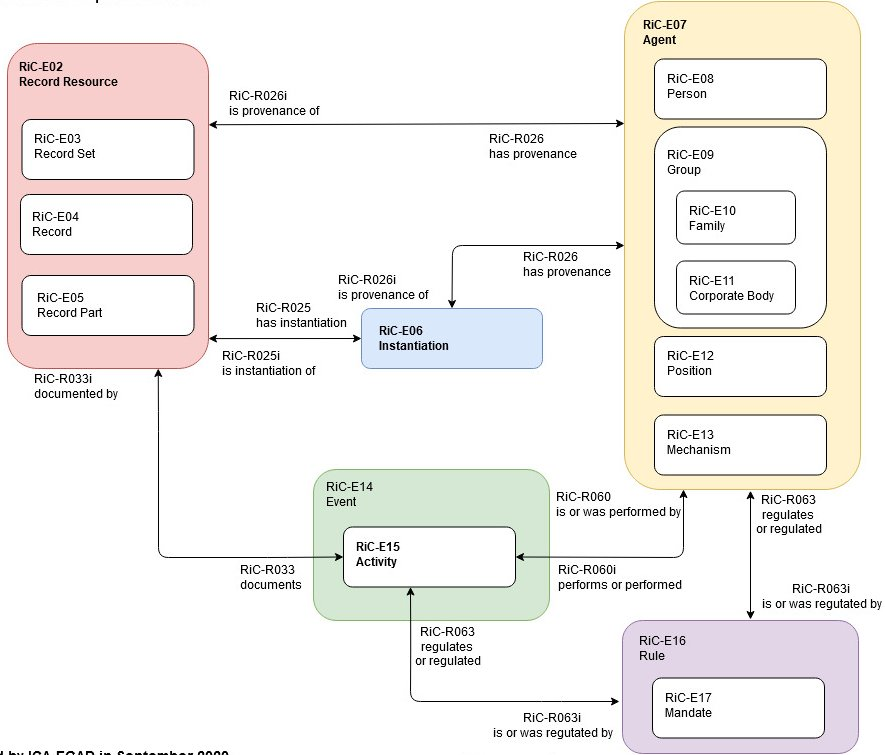
\includegraphics[width=16cm]{diagram_RiC-CM-overview-RiC-v0-2.jpg}
    \caption{Modèle conceptuel RiC-CM (\textit{Records in Contexts - Conceptual Model}), modélisé pour l'entrée des archives dans le Web de données. Le modèle utilise quatre entités de base (\textit{Record Resource}, \textit{Instanciation}, \textit{Agent} et \textit{Activity}. Voir https://www.ica.org/fr/records-in-contexts-modele-conceptuel (visité le 25/08/2023)}
    \label{fig:enter-label}
\end{figure}

\begin{figure}[h]
    \centering
    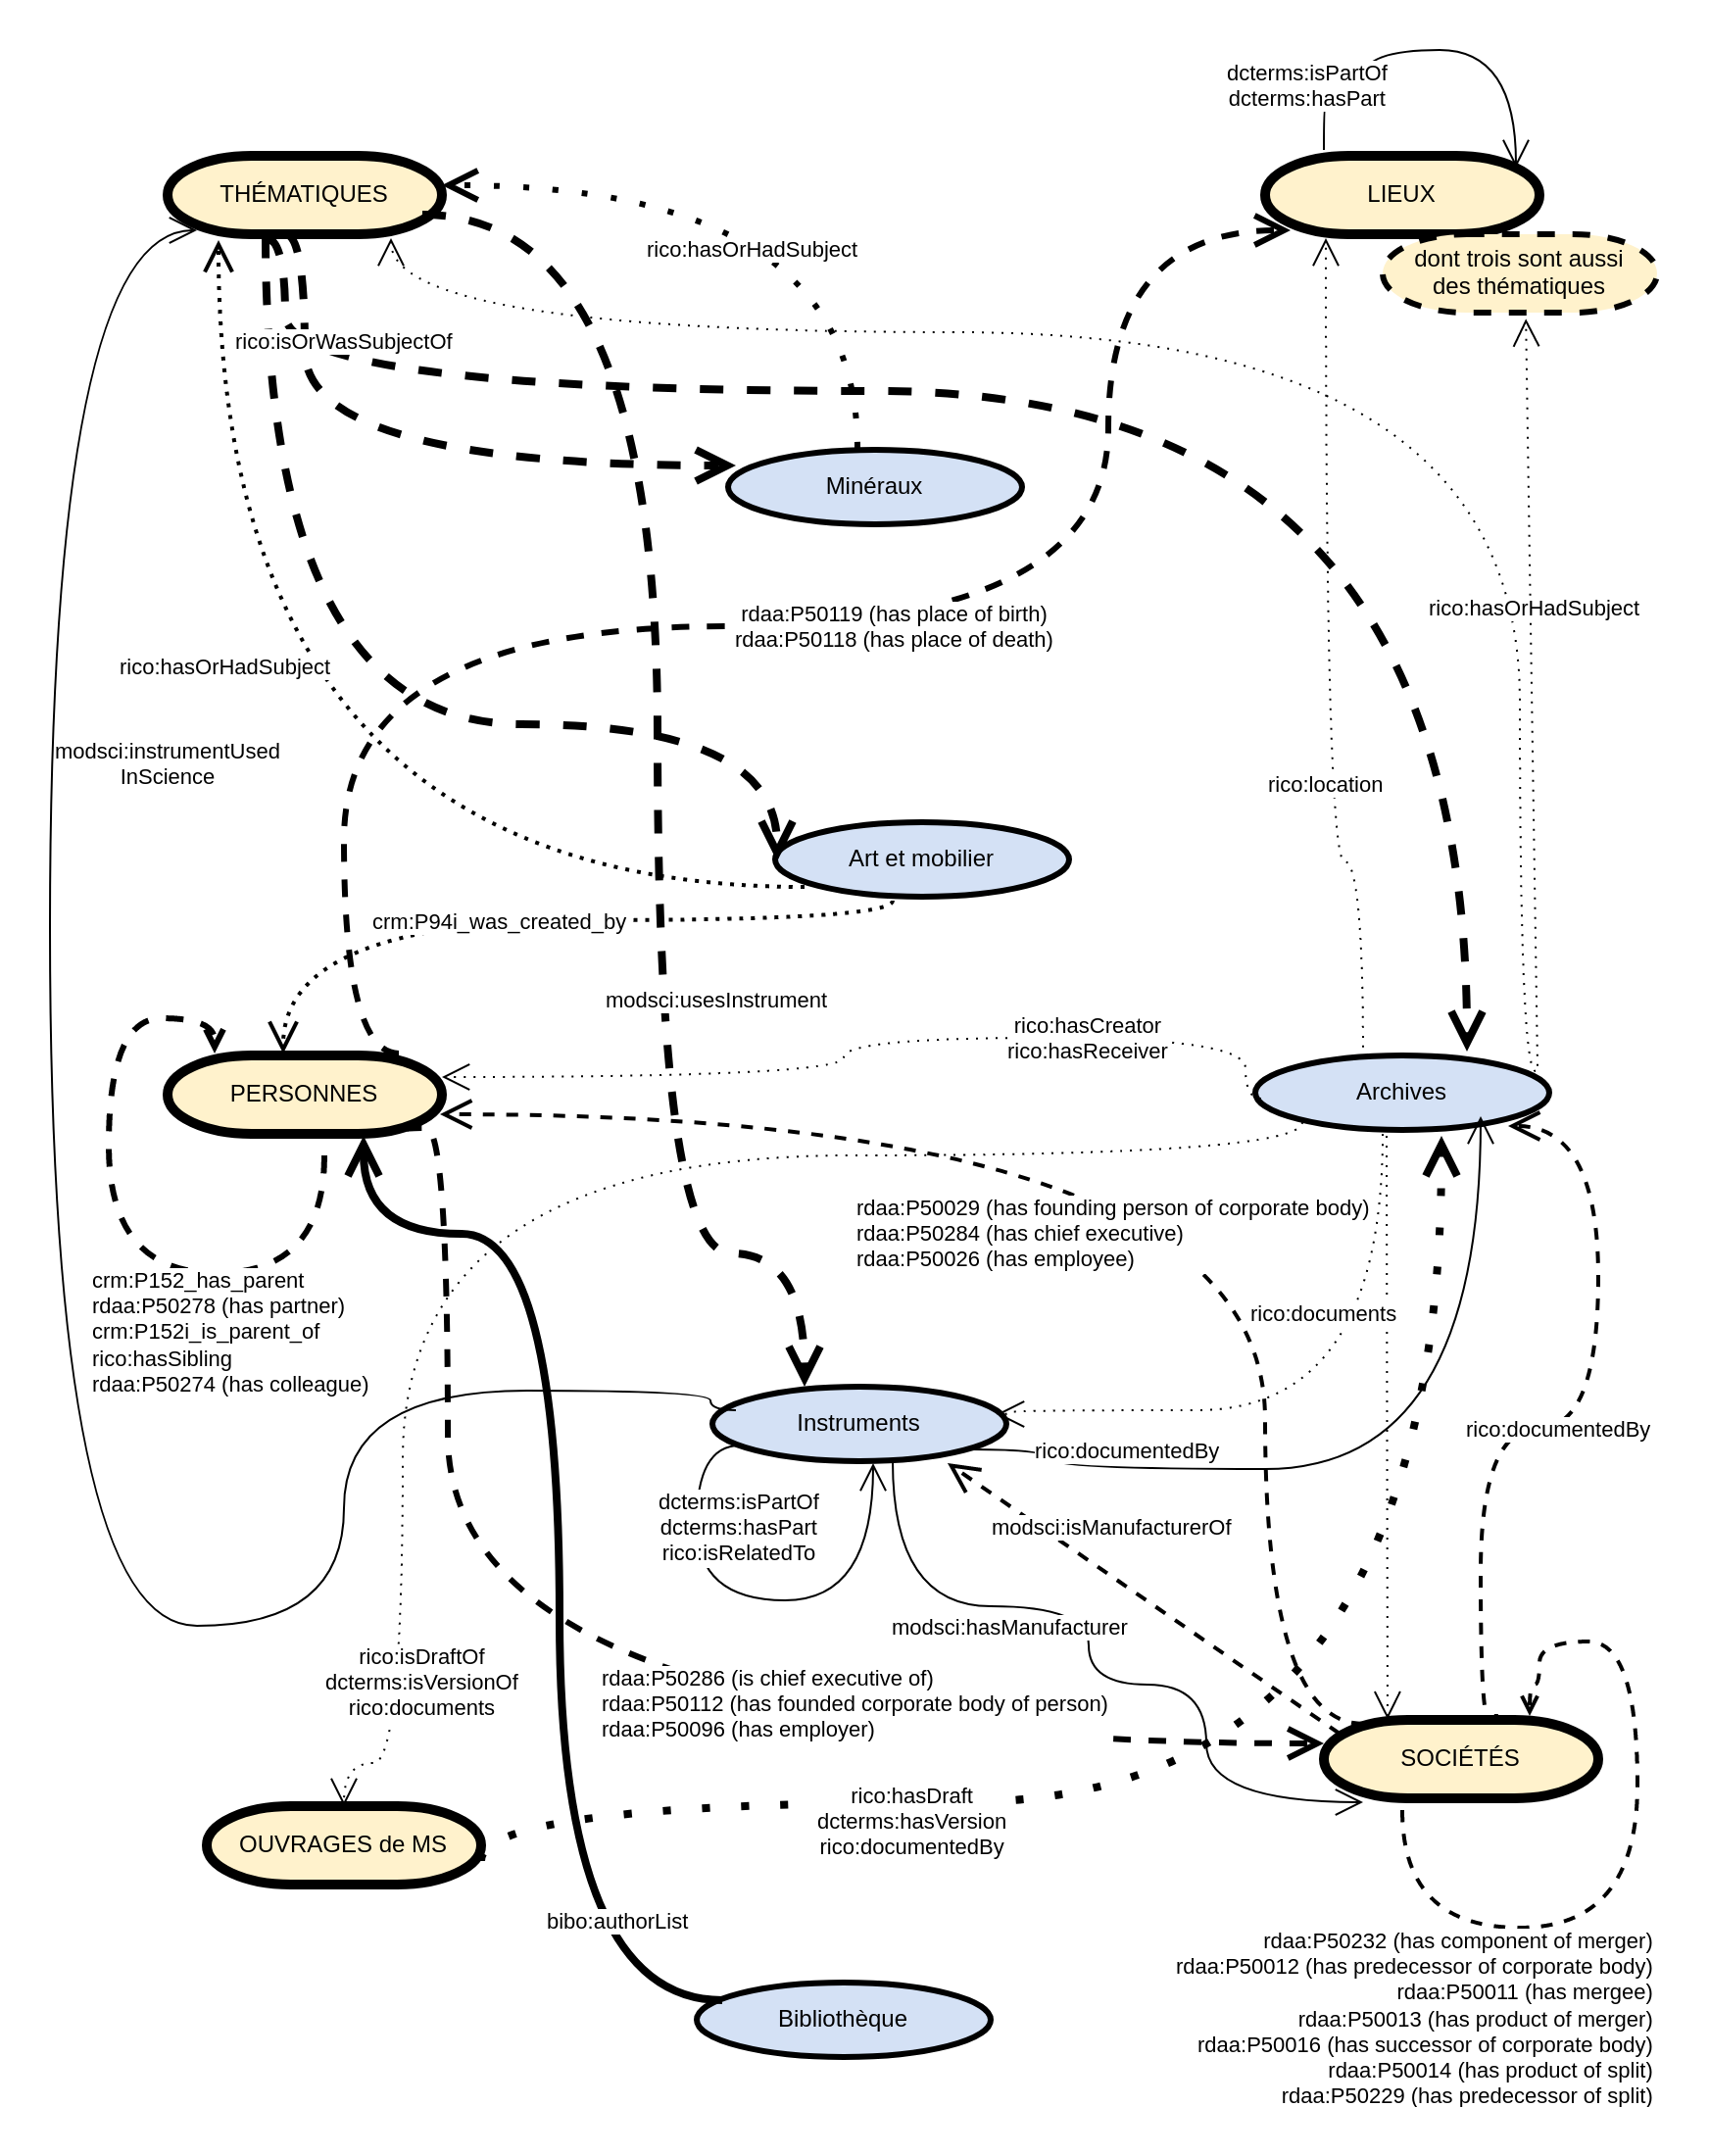
\includegraphics[width=16cm]{Lien entre items.png}
    \caption{Modèle conceptuel qui a servi de définition à la base de données de l'AAFS à Varagnes, lors de notre stage. Les entités correspondant aux différentes pièces d'inventaires sont en bleu; les entités de référence sont en jaune.}
    \label{fig:enter-label}
\end{figure}
        
        
	\chapter{Exemple de syntaxes du RDF}\label{annexe-syntaxes}
 \begin{figure}[h]
    \centering
    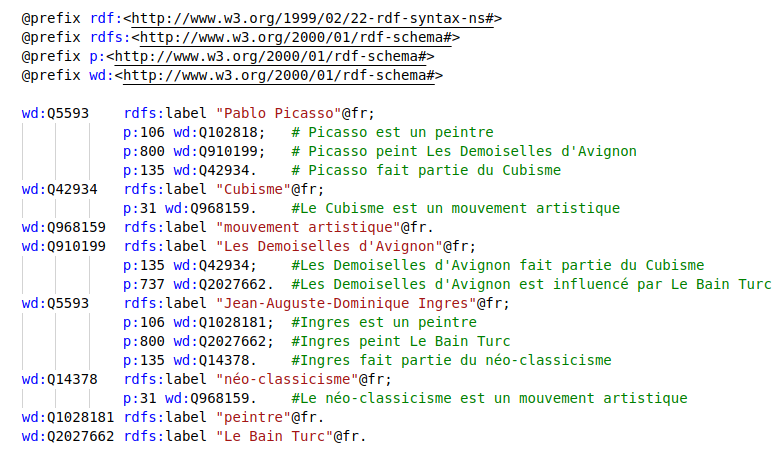
\includegraphics[width=16cm]{ANNEXE_B_TURTLE.png}
    \caption{Exemple d'une modélisation en Turtle. }
    \label{fig:enter-label}
\end{figure}

 \begin{figure}[h]
    \centering
    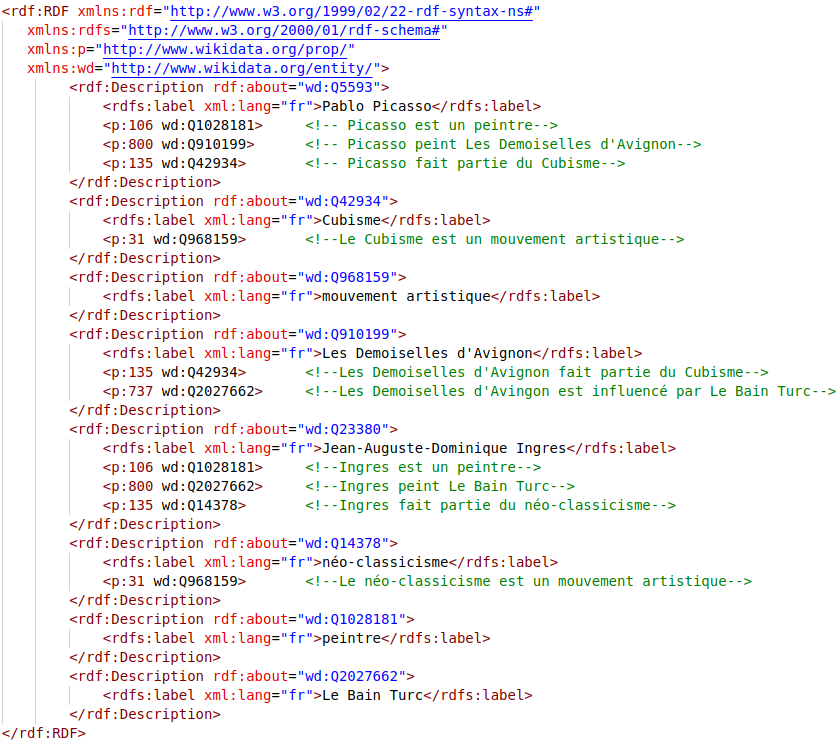
\includegraphics[width=16cm]{ANNEXE_A_RDF_XML.png}
    \caption{Exemple d'une syntaxe RDF/XML. Chaque entité est décrite en ouvrant une balise \textit{rdf:Description}, dont l'attribut \textit{rdf:about} va spécifier le sujet. Au sein de cette balise vont s'enchaîner les prédicats et leurs objets. Le prédicat \textit{rdfs:label} va donner un nom compréhensible pour un humain, tandis que les autres prédicats ont des entités en objet.}
    \label{fig:enter-label}
\end{figure}

	\chapter{Modélisations des données de l'AAFS}\label{modelisations-AAFS}
 \begin{figure}[h]
    \centering
    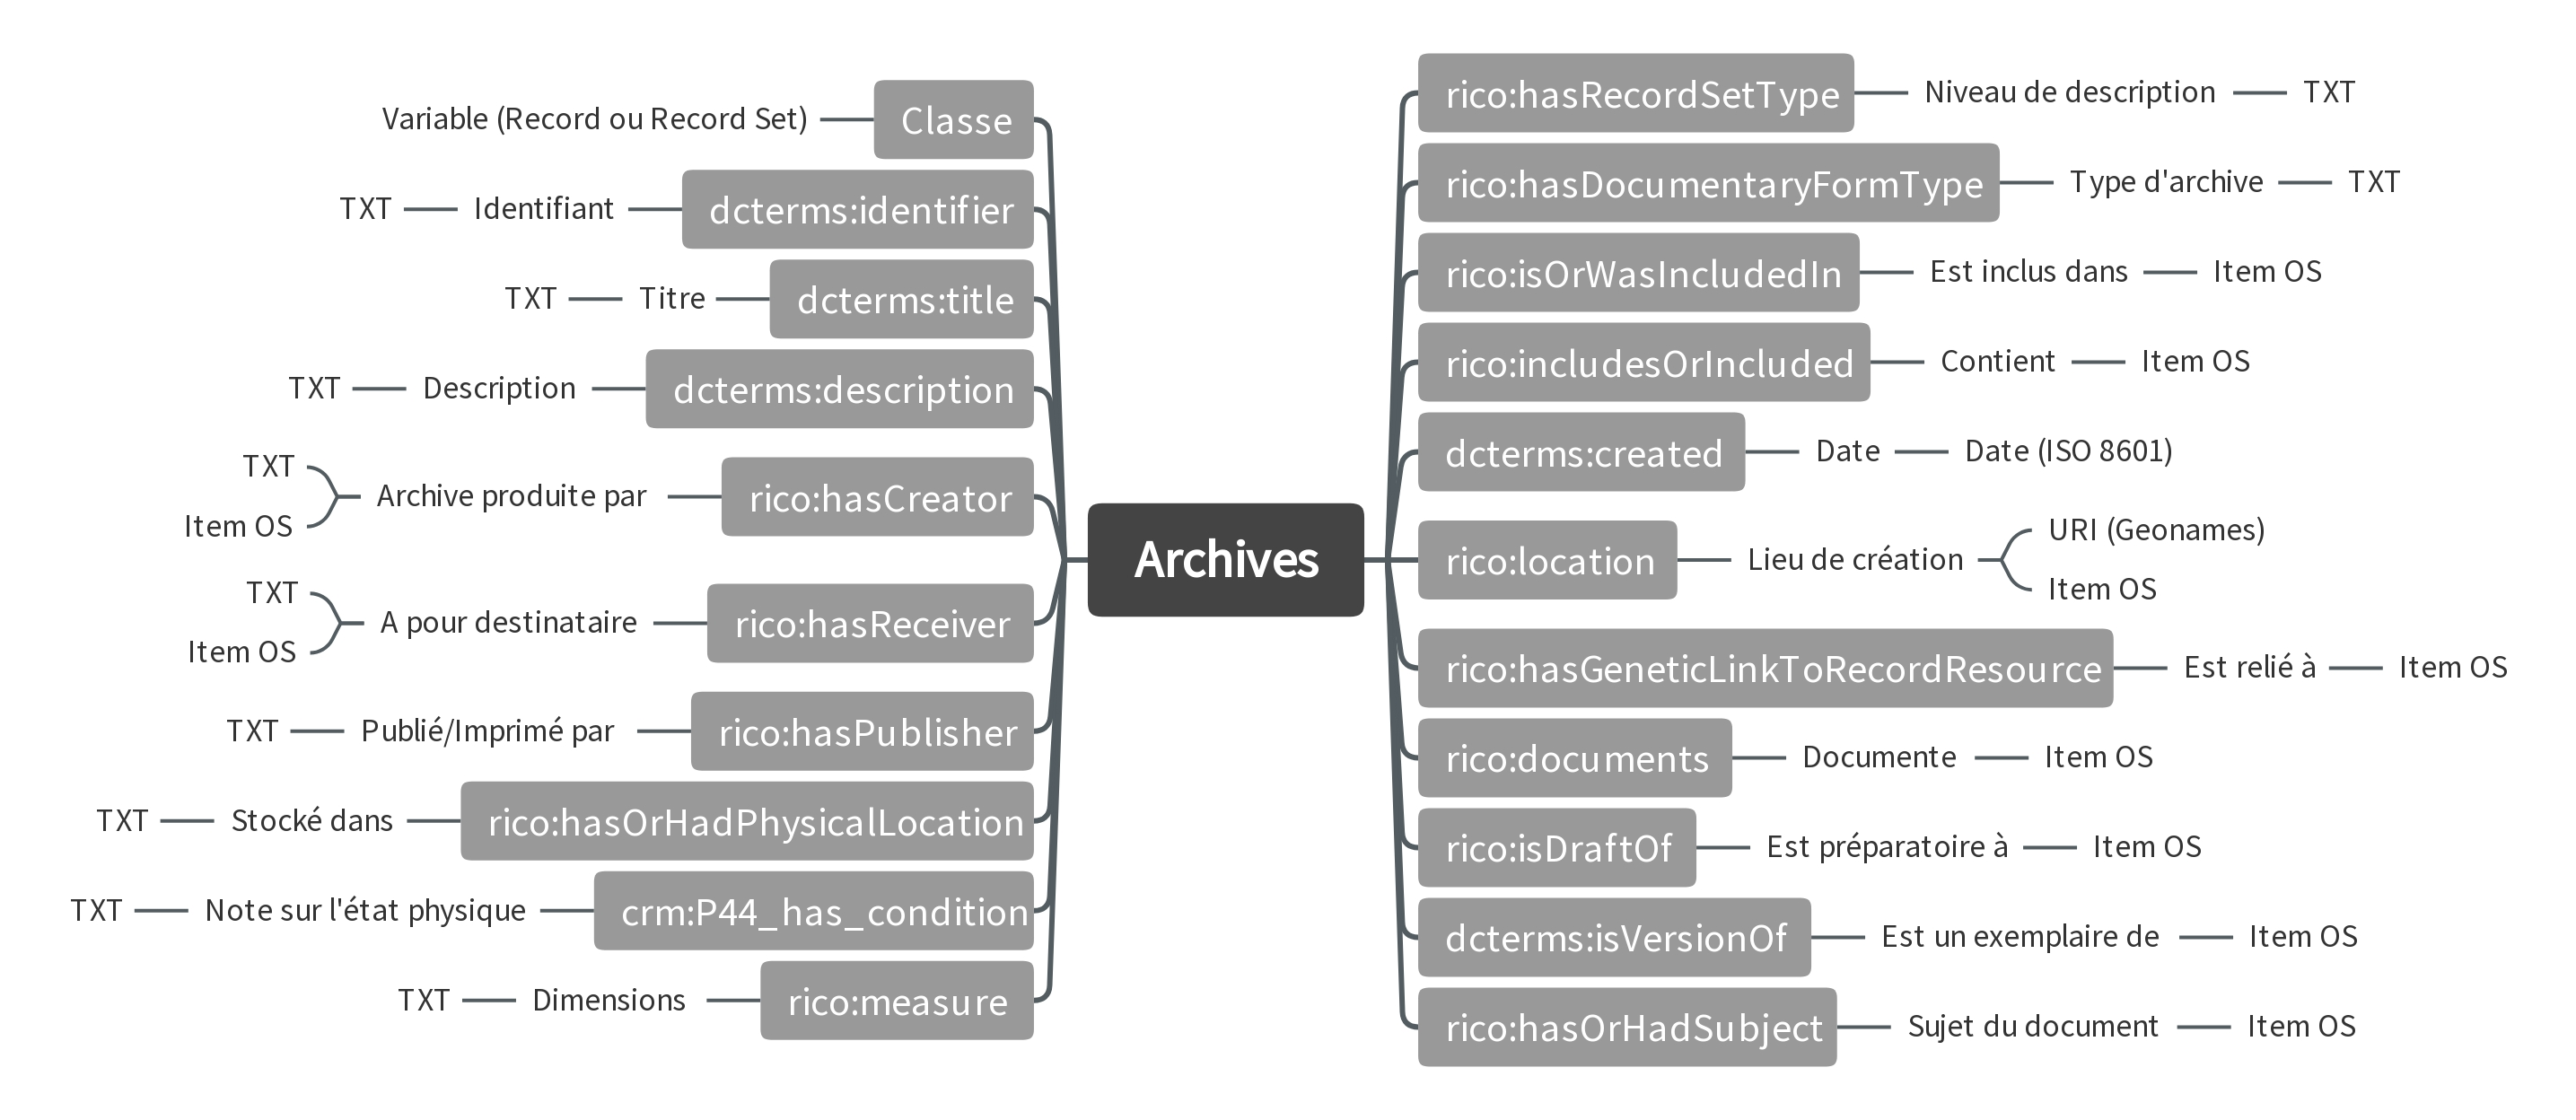
\includegraphics[width=16cm]{Archives (1).jpg}
    \caption{Modélisation des données d'archives pour la base de l'AAFS.}
    \label{fig:enter-label}
\end{figure}

 \begin{figure}[h]
    \centering
    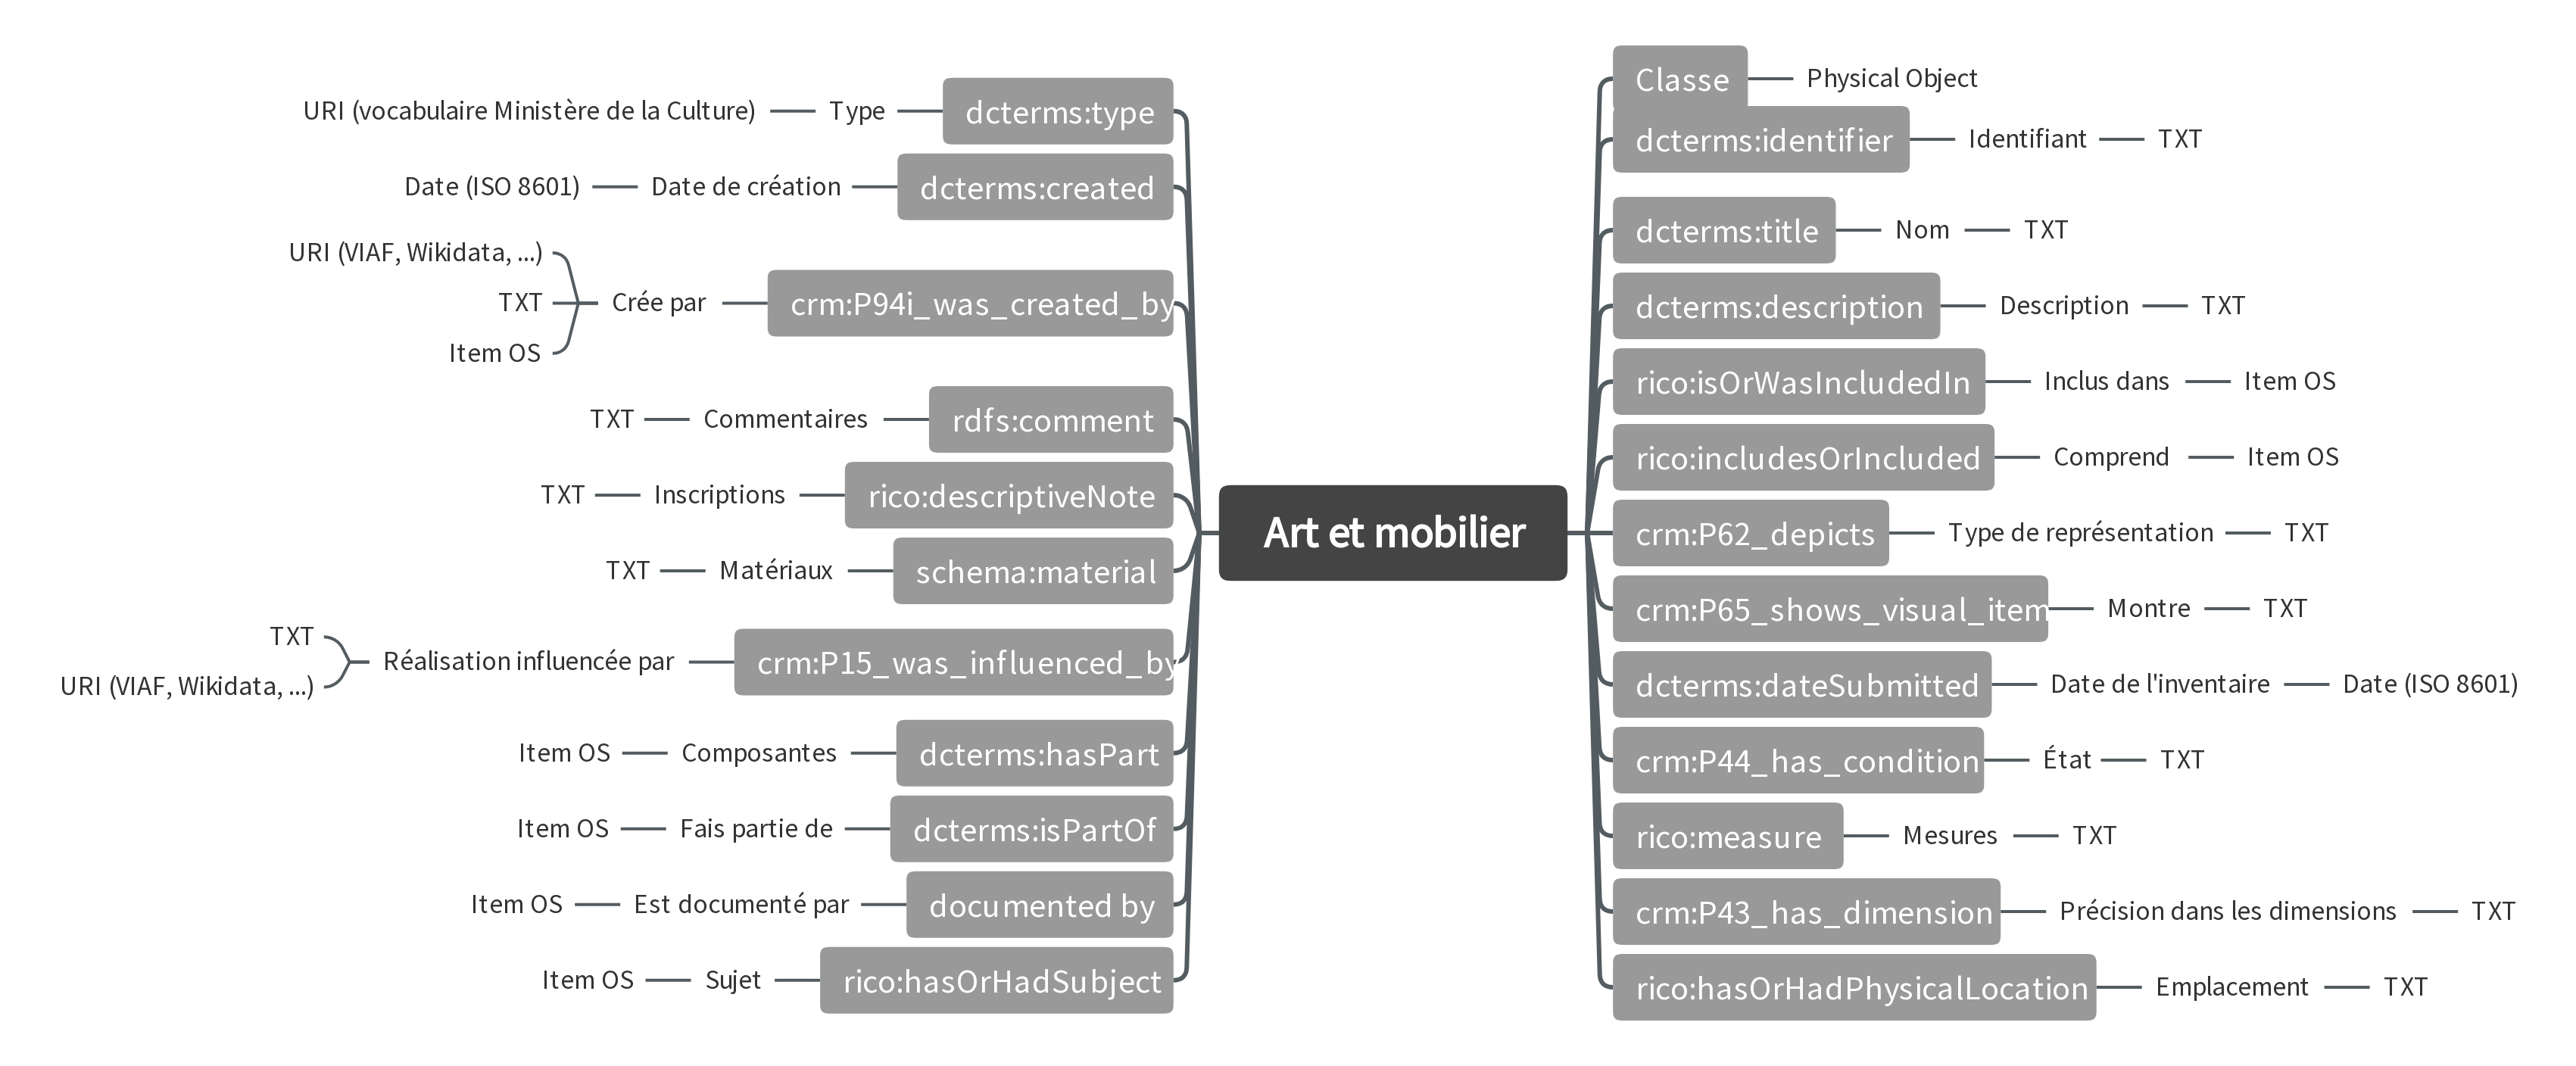
\includegraphics[width=16cm]{Art et mobilier.jpg}
    \caption{Modélisation des données du mobilier pour la base de l'AAFS.}
    \label{fig:enter-label}
\end{figure}



 \begin{figure}[h]
    \centering
    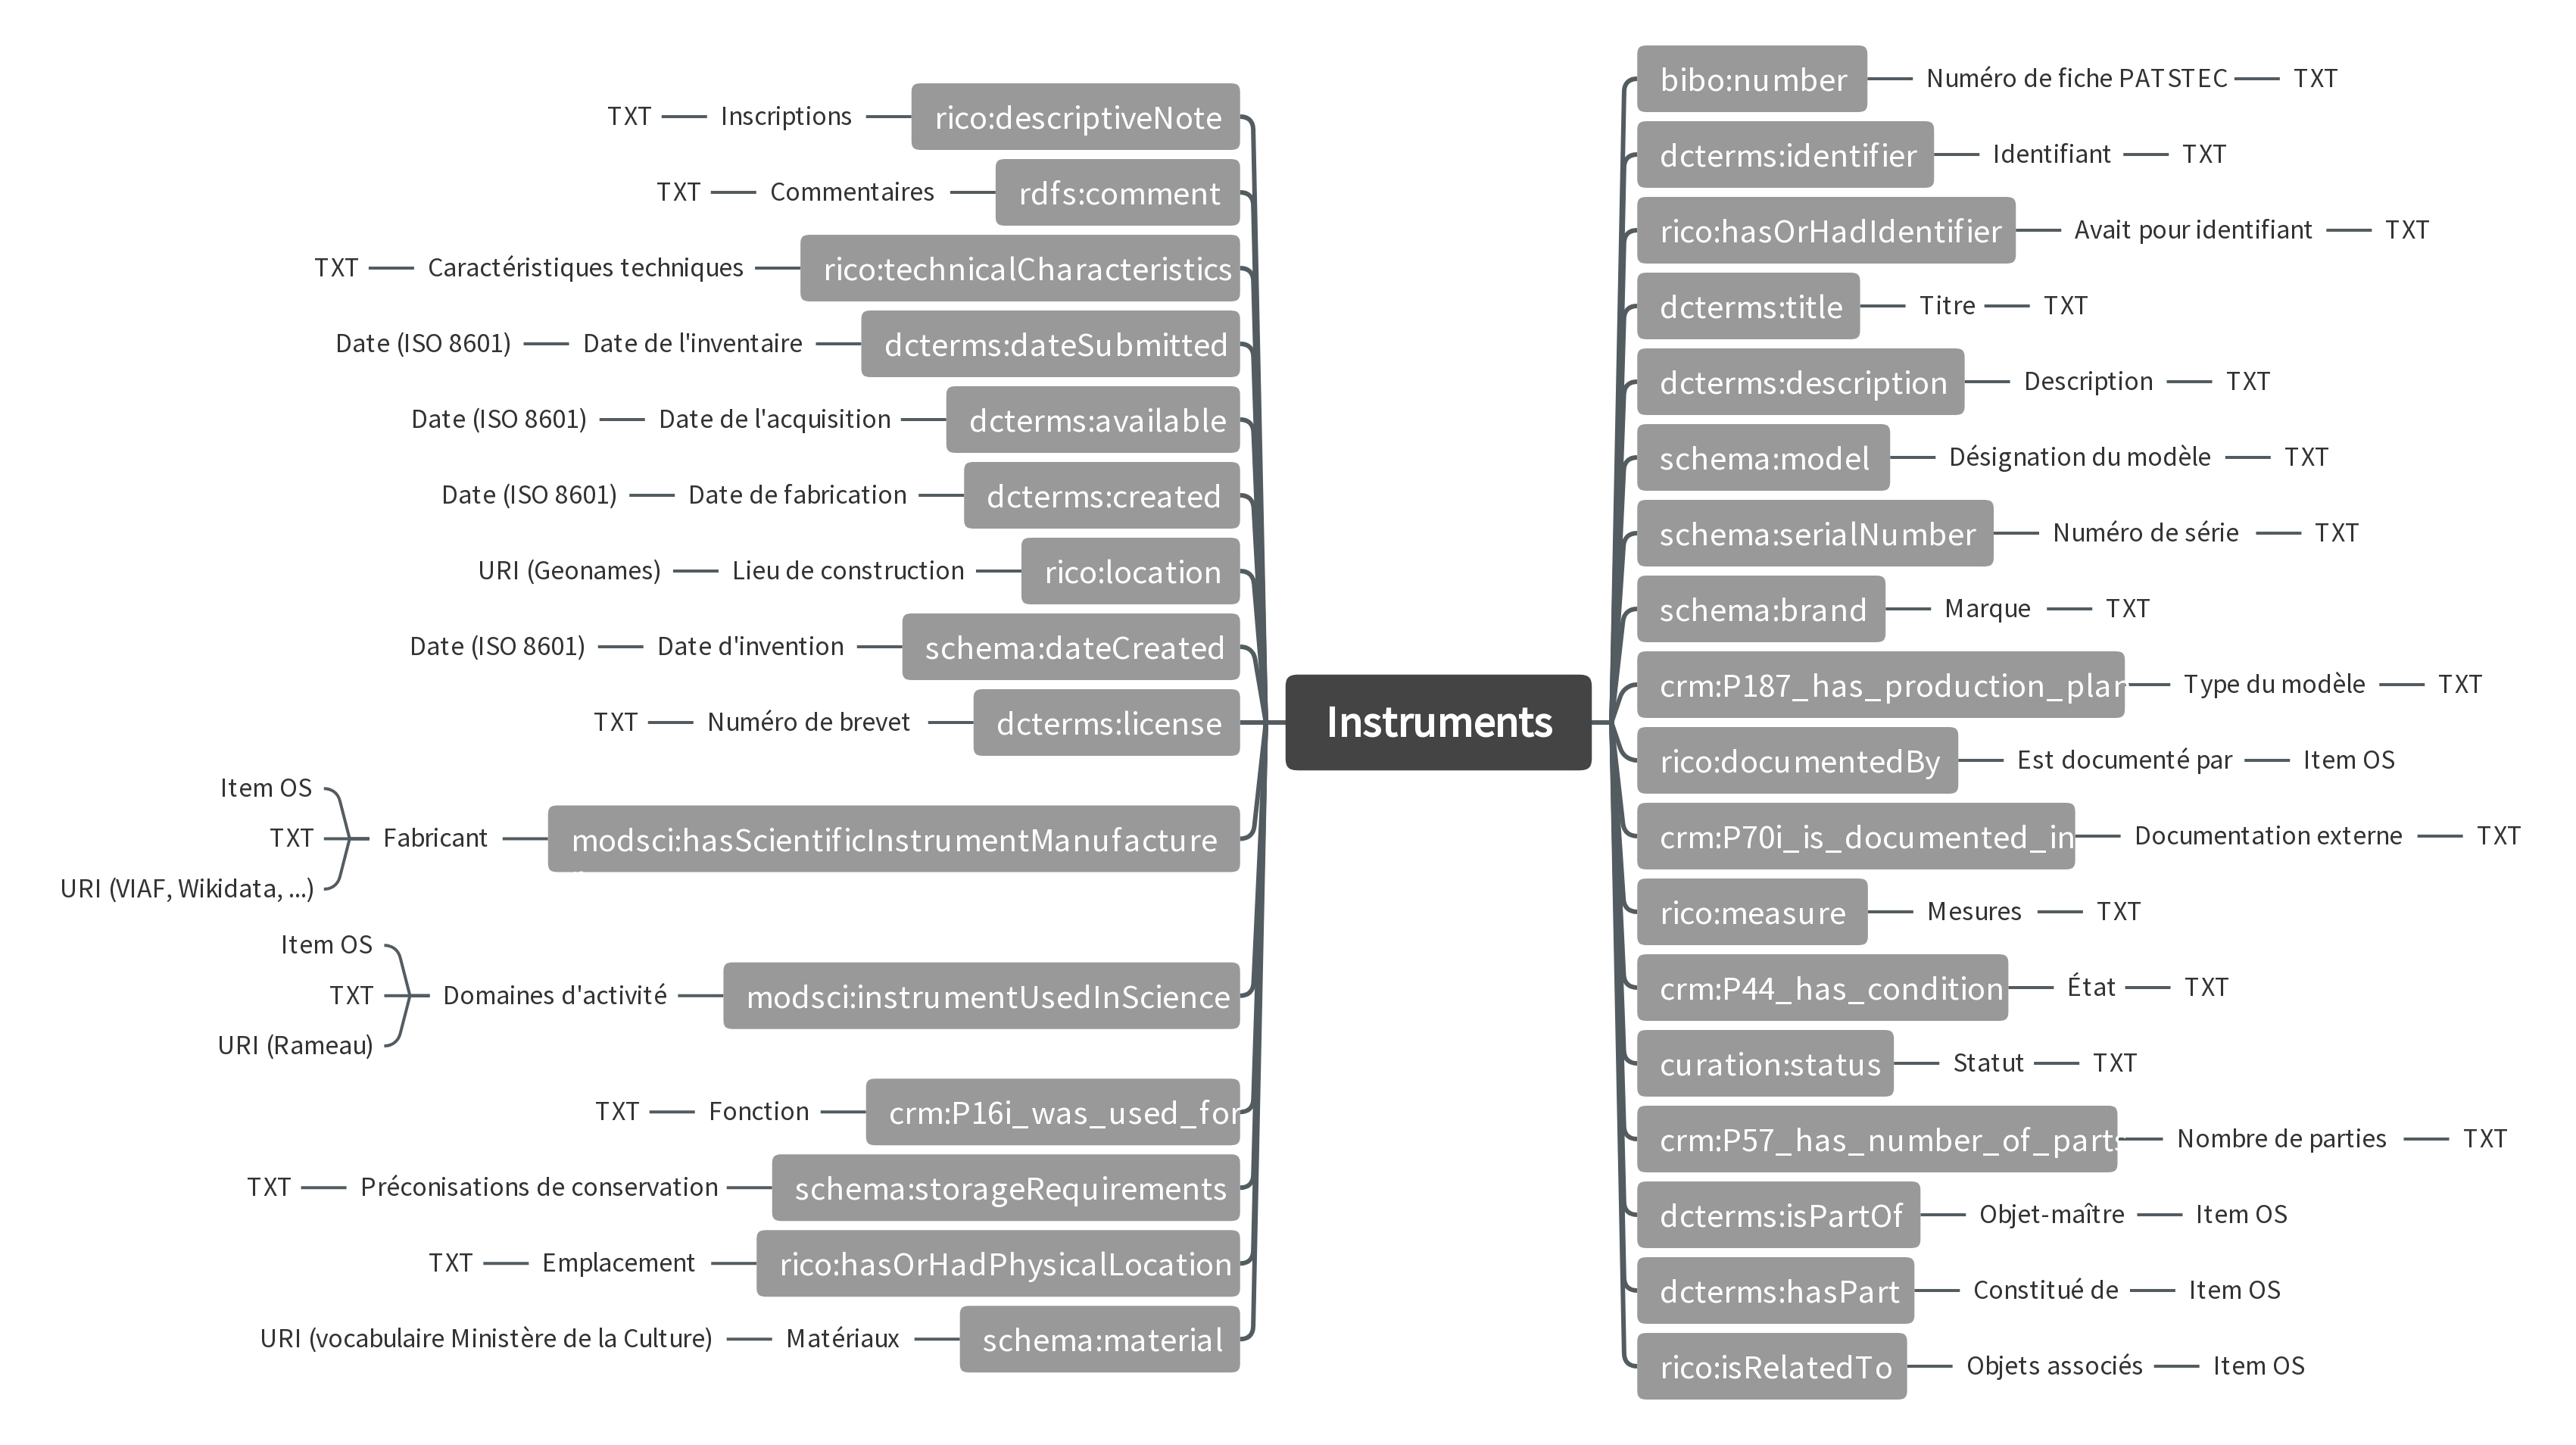
\includegraphics[width=16cm]{Instruments.jpg}
    \caption{Modélisation des données du patrimoine technique pour la base de l'AAFS.}
    \label{fig:enter-label}
\end{figure}

 \begin{figure}[h]
    \centering
    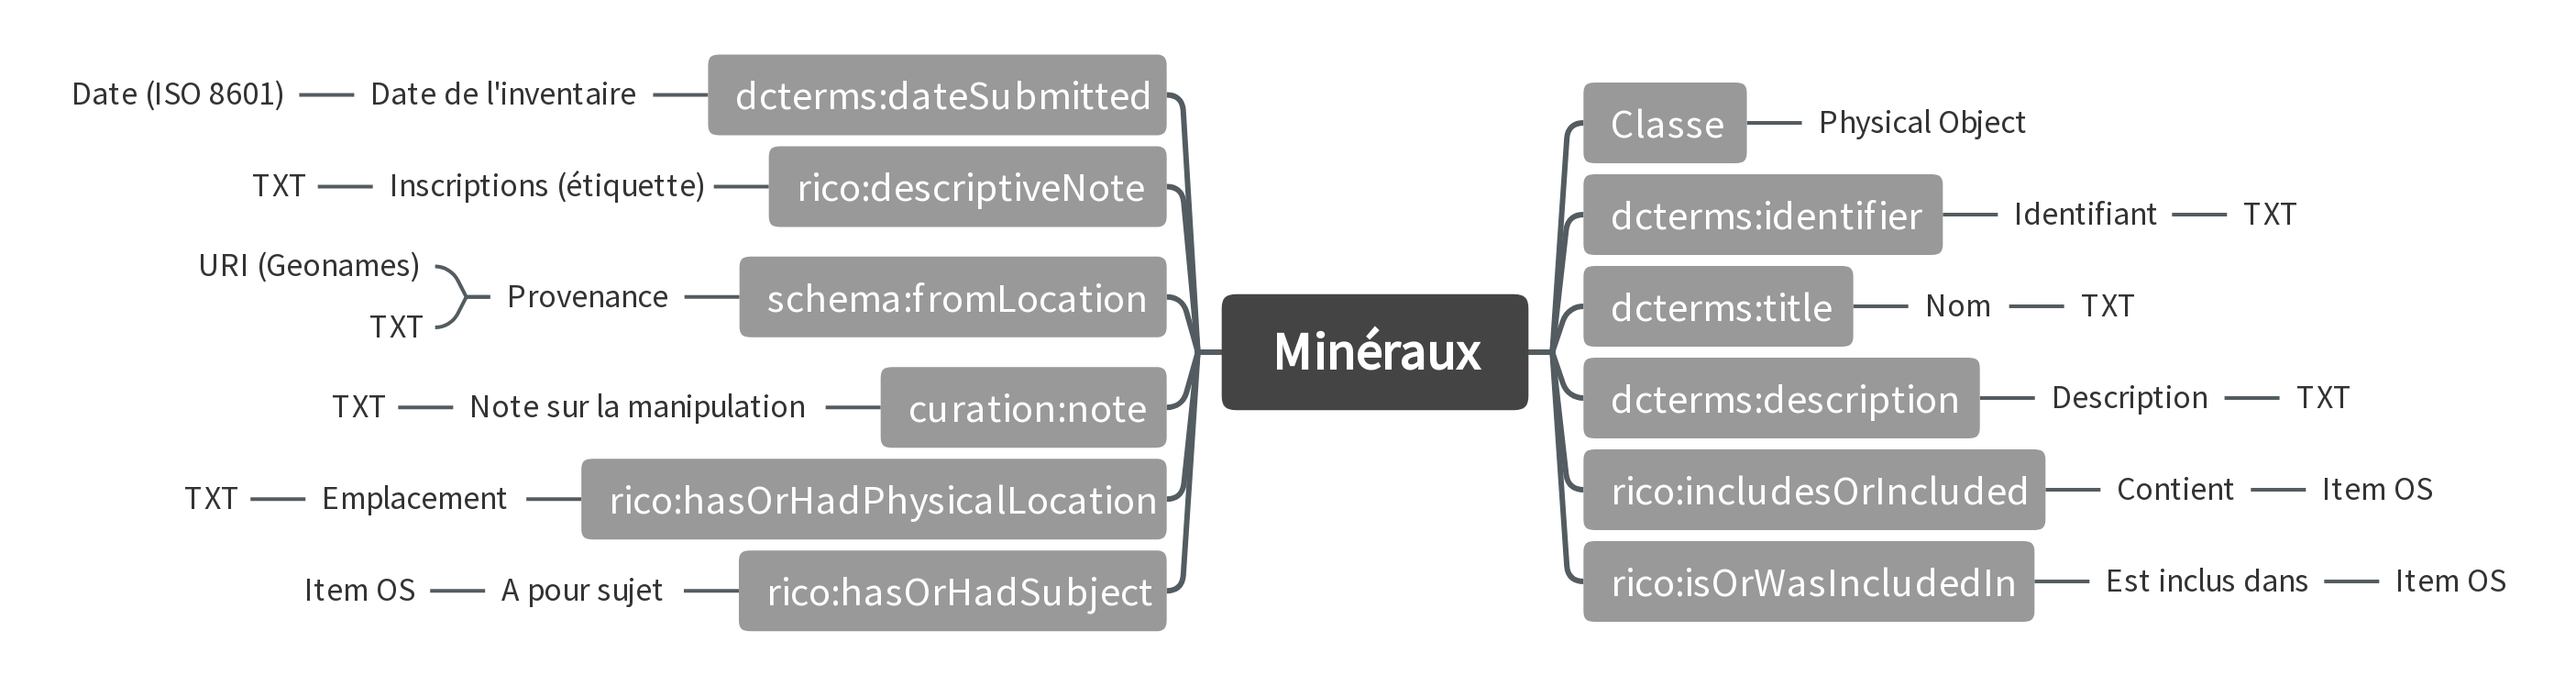
\includegraphics[width=16cm]{Minéraux.jpg}
    \caption{Modélisation des données de minéralogie pour la base de l'AAFS.}
    \label{fig:enter-label}
\end{figure}

 \begin{figure}[h]
    \centering
    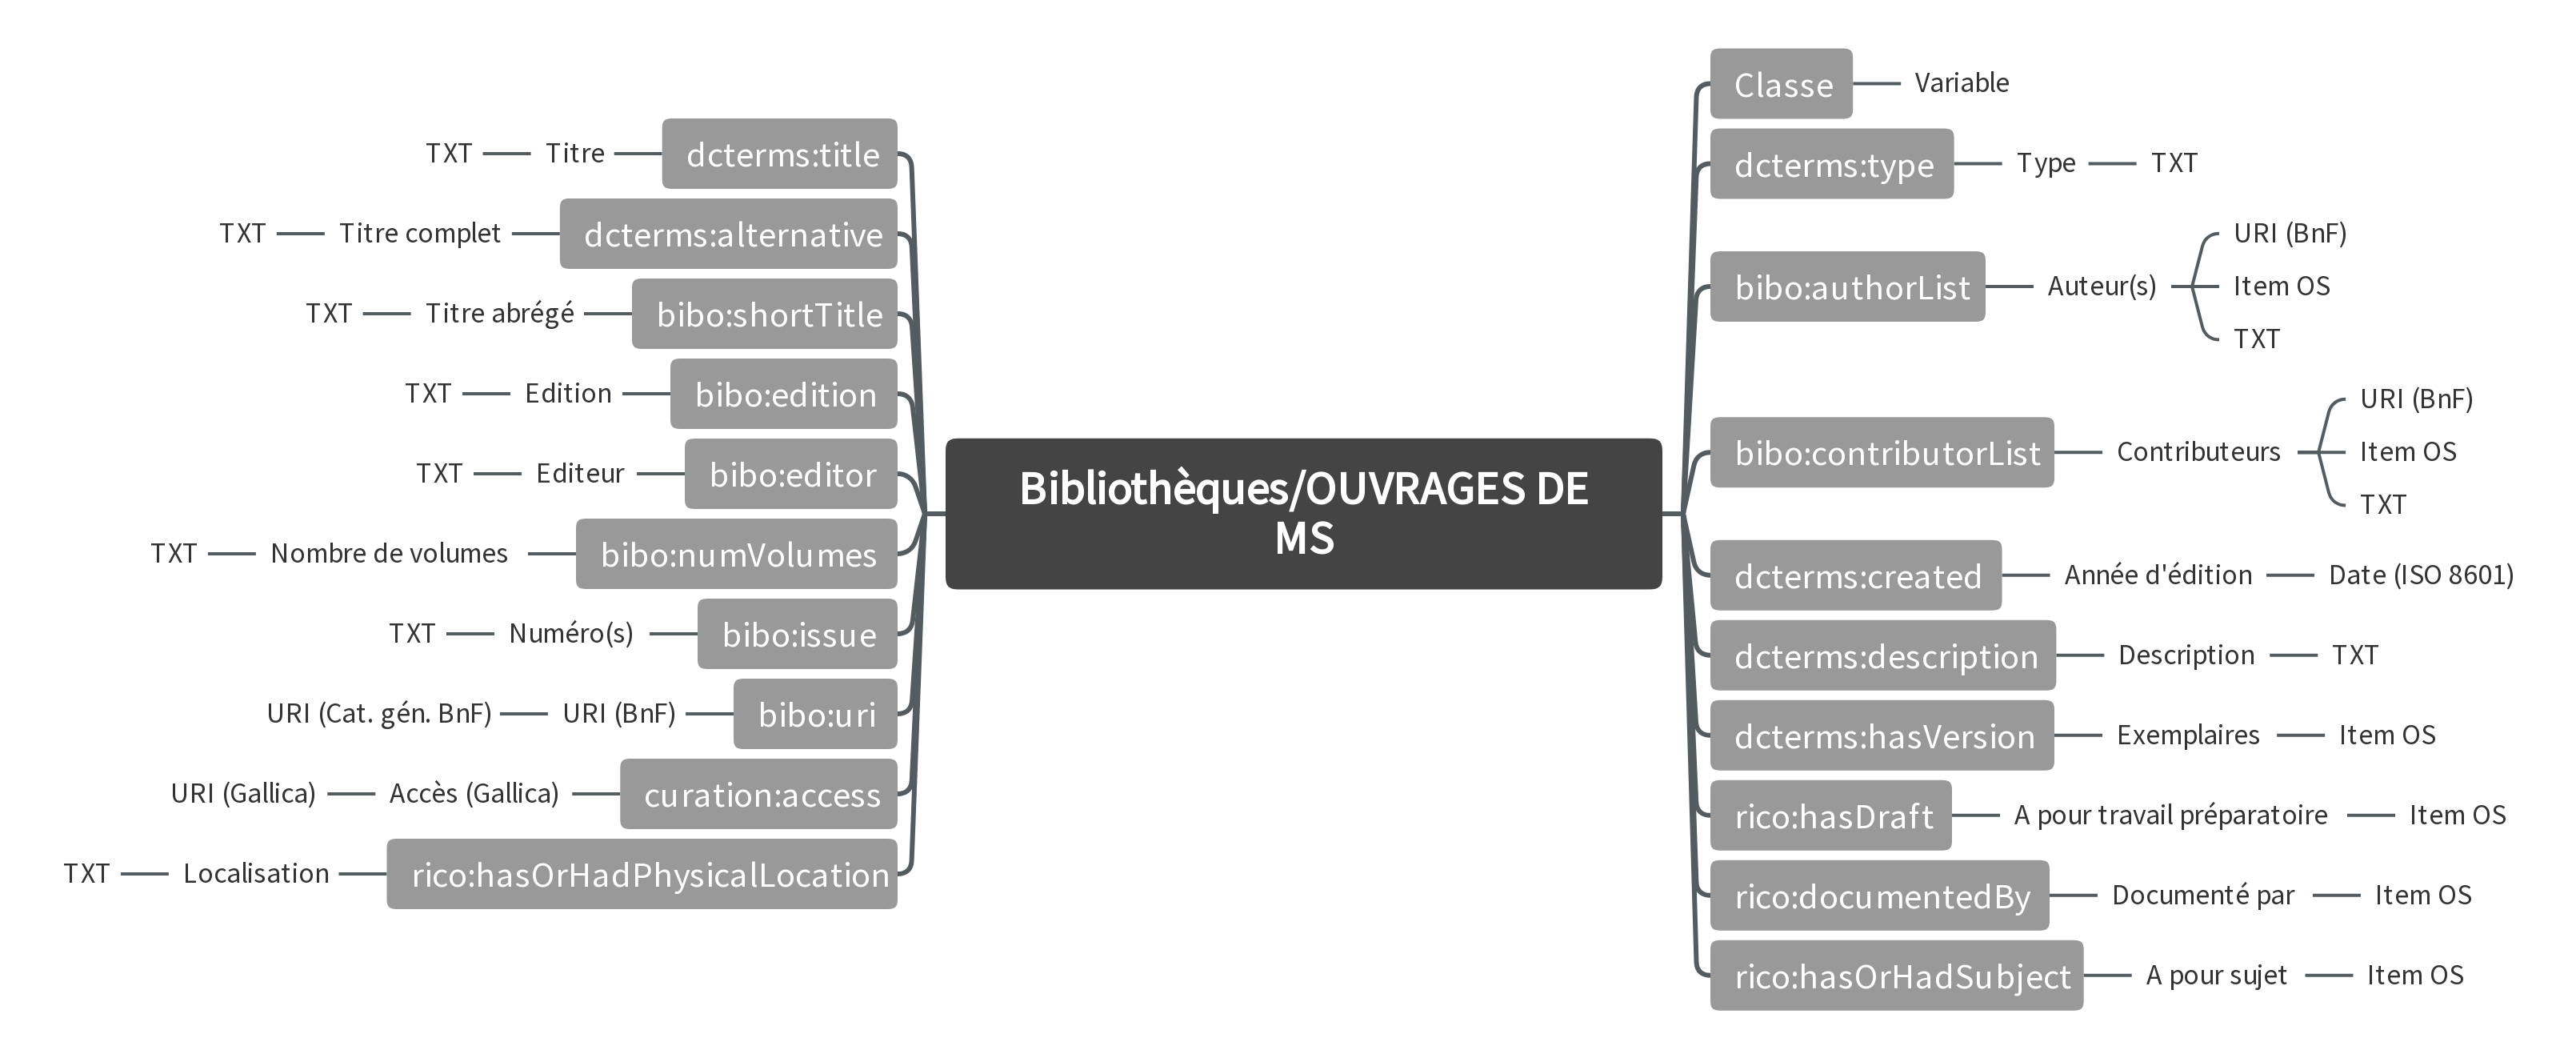
\includegraphics[width=16cm]{Bibliothèques_Ouvrages de MS (1).jpg}
    \caption{Modélisation des données bibliographiques pour la base de l'AAFS.}
    \label{fig:enter-label}
\end{figure}

 \begin{figure}[h]
    \centering
    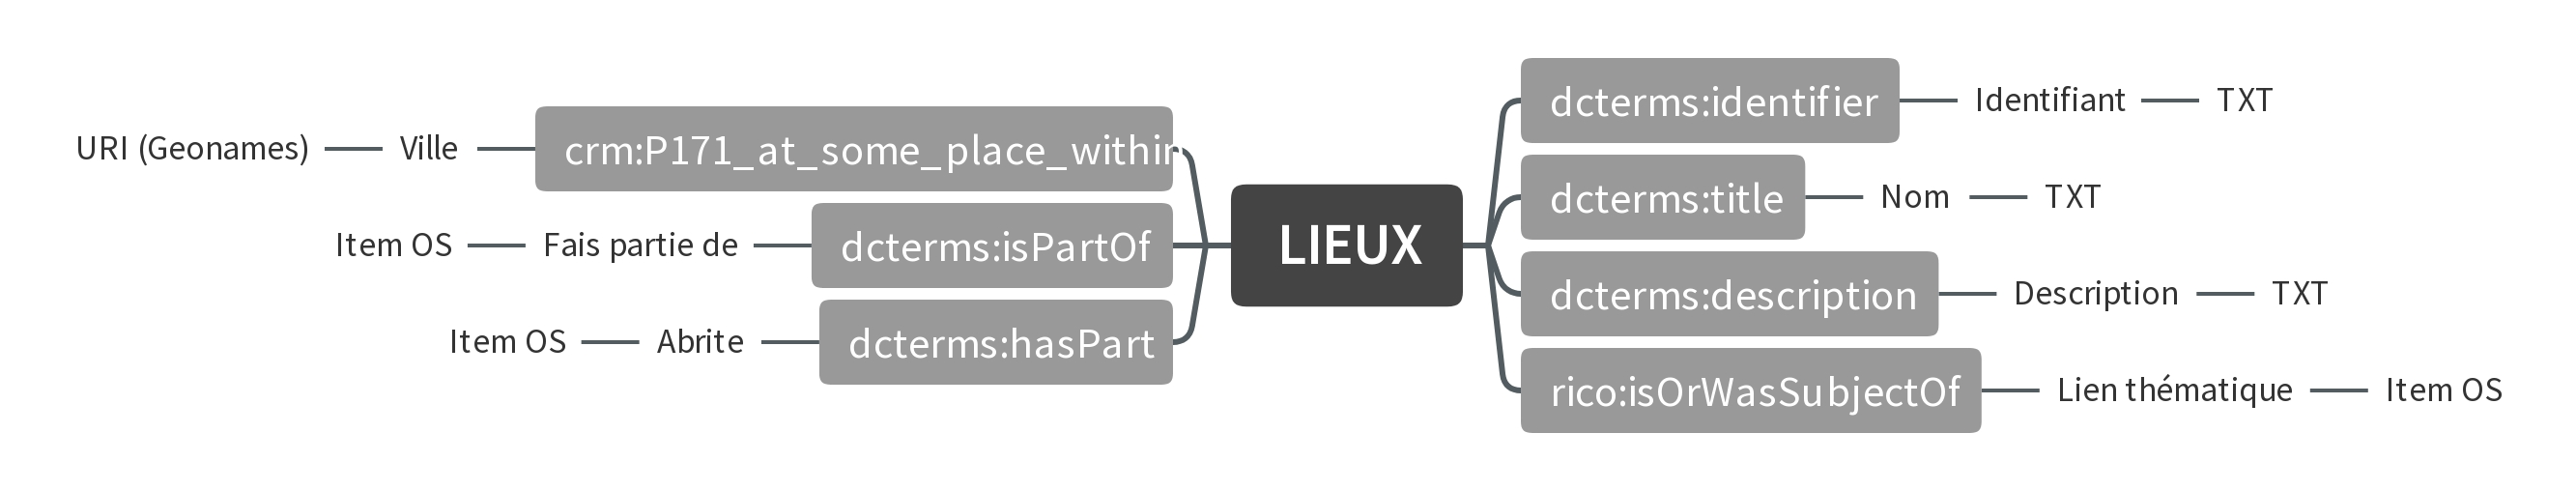
\includegraphics[width=16cm]{LIEUX.jpg}
    \caption{Modélisation des données de référence de lieux pour la base de l'AAFS.}
    \label{fig:enter-label}
\end{figure}


 \begin{figure}[h]
    \centering
    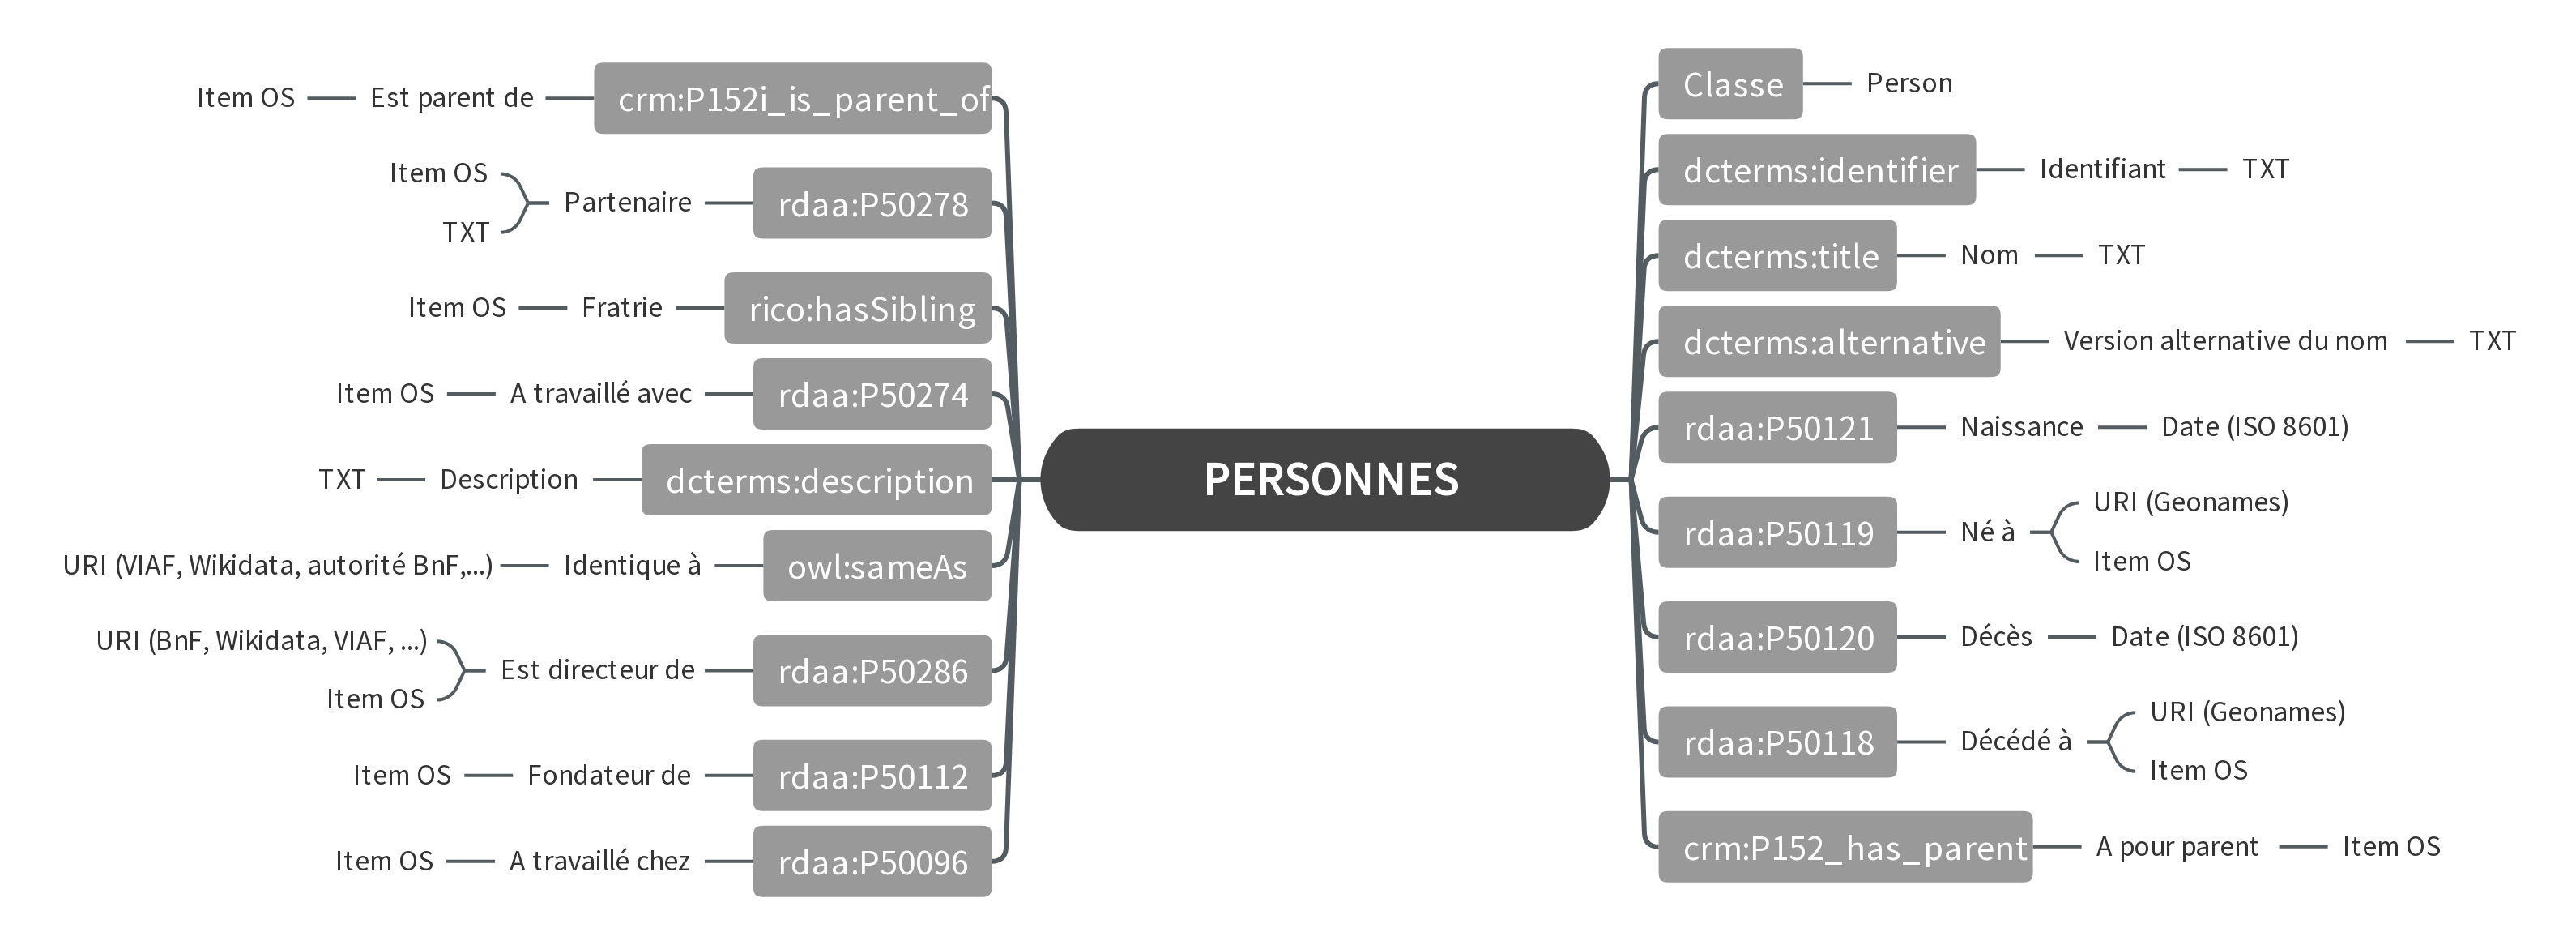
\includegraphics[width=16cm]{PERSONNES (7).jpg}
    \caption{Modélisation des données de référence de personnes pour la base de l'AAFS.}
    \label{fig:enter-label}
\end{figure}


 \begin{figure}[h]
    \centering
    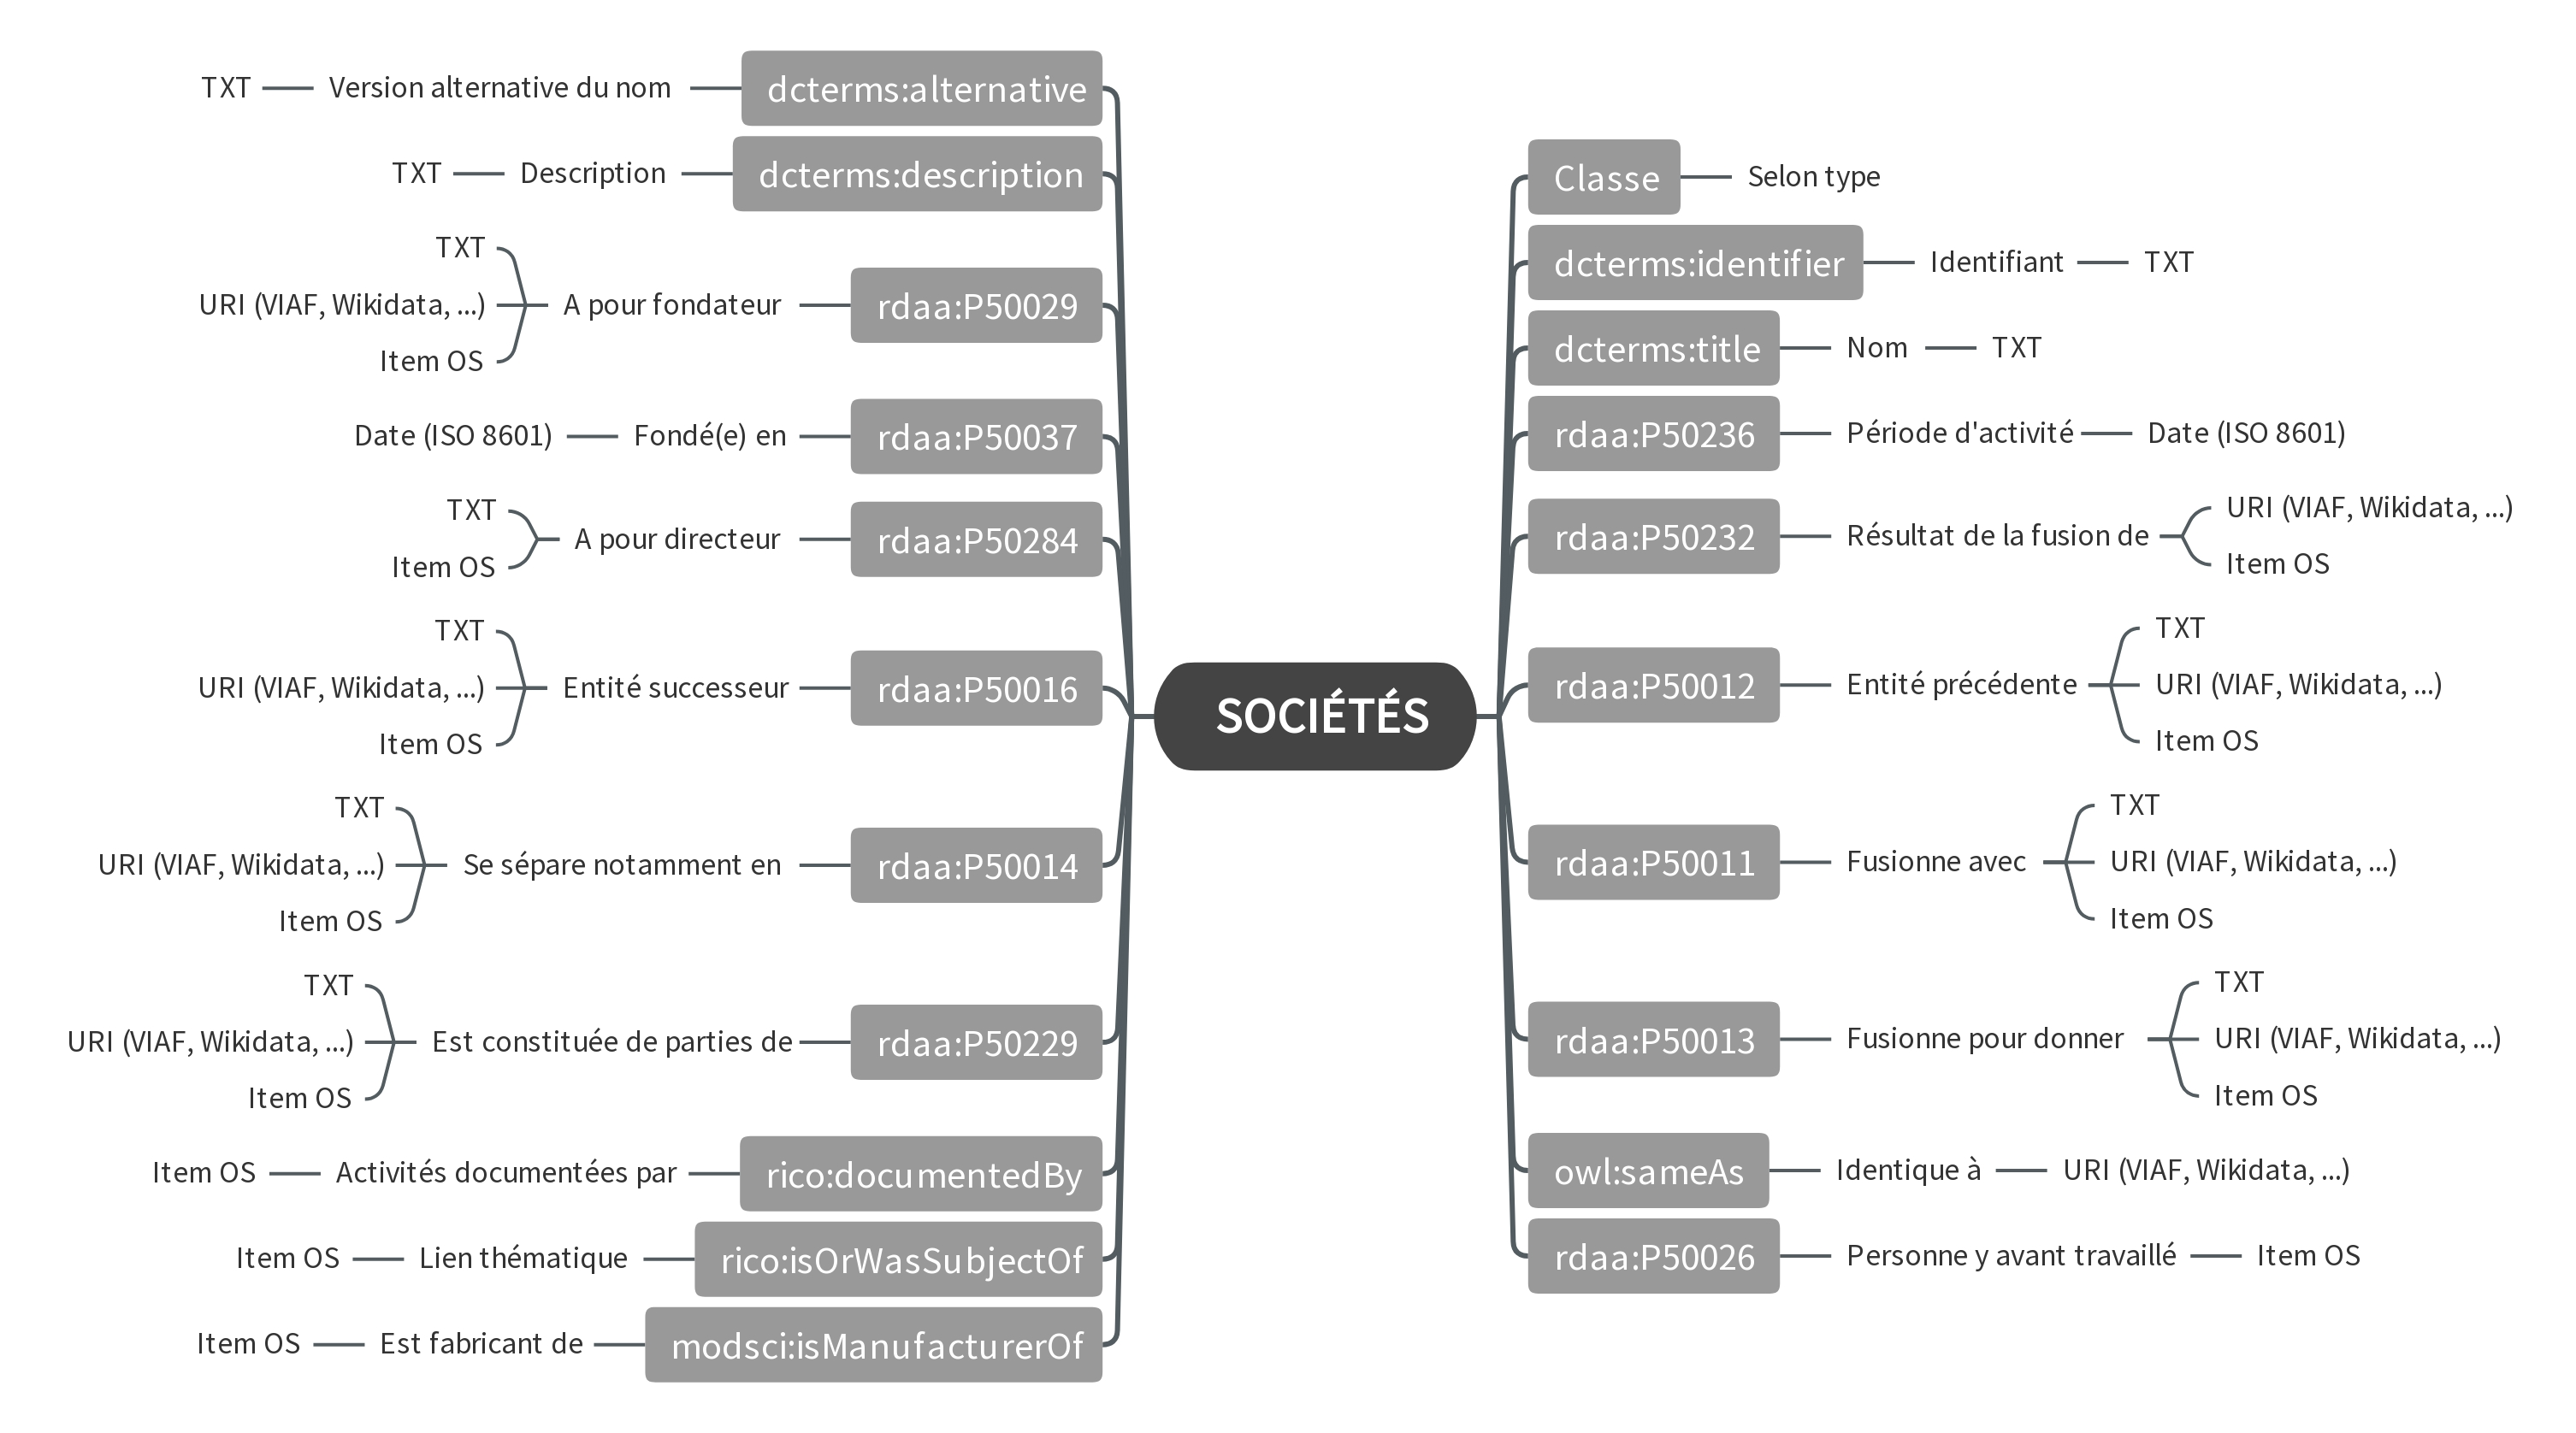
\includegraphics[width=16cm]{SOCIÉTÉS (2).jpg}
    \caption{Modélisation des données de référence des agents collectifs pour la base de l'AAFS.}
    \label{fig:enter-label}
\end{figure}


 \begin{figure}[h]
    \centering
    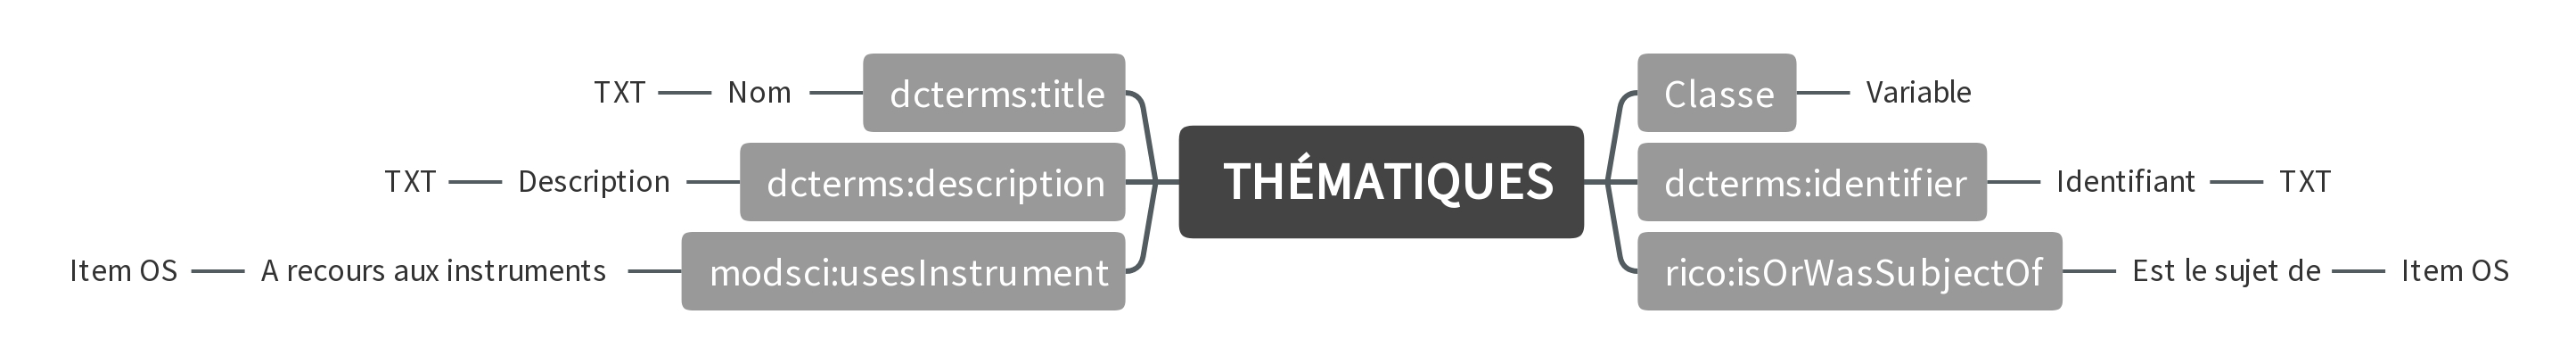
\includegraphics[width=16cm]{THÉMATIQUES.jpg}
    \caption{Modélisation des données de référence de thématiques pour la base de l'AAFS.}
    \label{fig:enter-label}
\end{figure}

\chapter{Modélisation orientée Évènement}\label{model-cidoc-crm}

\begin{figure}[h]
    \centering
    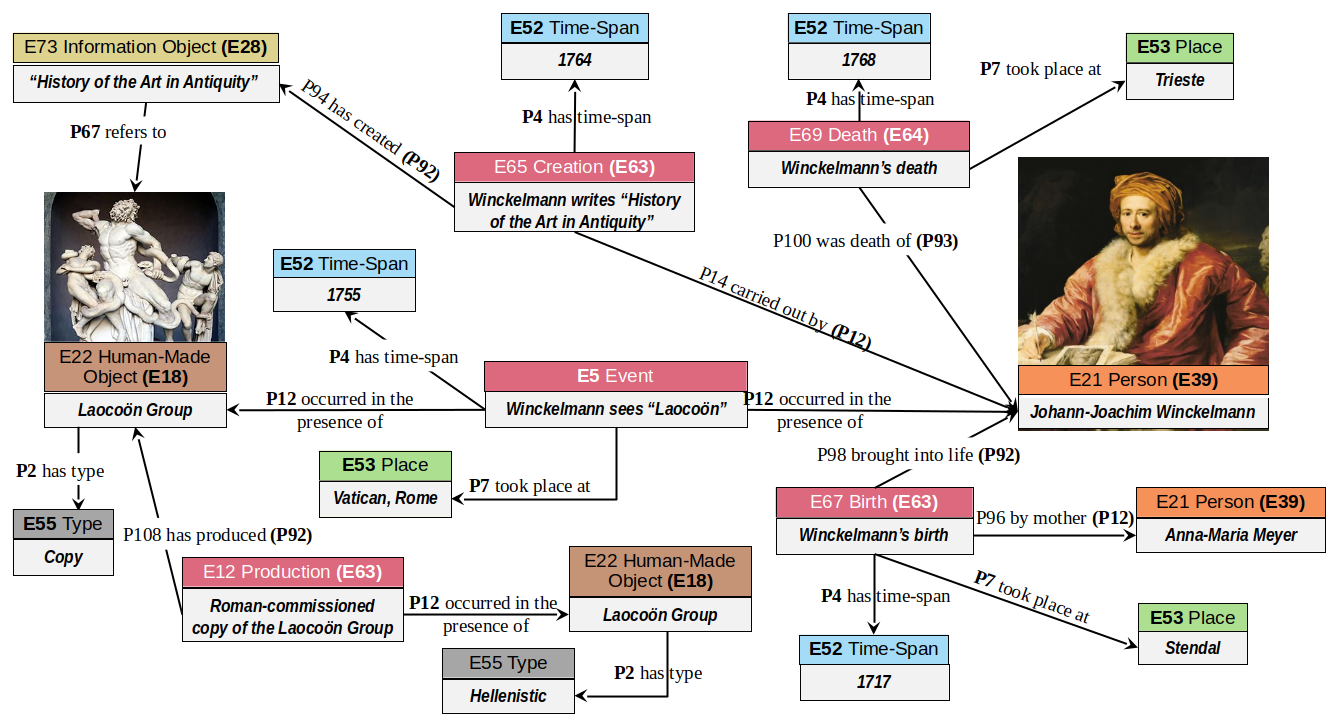
\includegraphics[width=22cm, angle=90]{471-001-MD-Laokoon_new_colors(17-2-2020).png}
    \caption{Exemple de modélisation du CIDOC-CRM (\url{https://www.cidoc-crm.org/data_examples}, visité le 26/08/2023)}
    \label{fig:enter-label}
\end{figure}
   
	
	\backmatter

% index à mettre ici si index	
%	\printindex

% glossaire si glossaire
%	\printglossaries

% si figures
%	\listoffigures

% si tables
%	\listoftables

	\tableofcontents
	
\end{document}